\documentclass[11pt,twoside,a4paper,BCOR8.25mm,DIV10,headsepline,footsepline,]{scrbook}
%------------------------------------------------------------------------------
%- PAKETE
%------------------------------------------------------------------------------
	%DIN A4
		\usepackage{a4}   

	%Fancy headers
		\usepackage{fancyhdr}
	
	%Sprache einstellen (Inhaltsverzeichnis, ...)
		\usepackage[english, ngerman]{babel} %american,italian,german
	
	%Euro Zeichen
		\usepackage{eurosym}	
		
		\usepackage[bookmarks=true,
					bookmarksopen=true,
   					% Lesezeichen ausgeklappt
					bookmarksnumbered=true,
					colorlinks=true,
				   	%Einf�rbung von Links
					linkcolor=black
					% Linkfarbe: schwarz					
					]
				    % Anzeige der Kapitelzahlen am Anfang der Namen der Lesezeichen
				   {hyperref}
		
	% Vereinfachtes Eingeben von Leerschl�gen hinter Shortcut-Commands
	% Beispiel: \newcommand{\DNA}{desoxyribose nucleid acid\xspace}
		\usepackage{xspace}
	
	%Sortierte Literaturverweise
		\usepackage{cite}
			
	%Grafiken
		\usepackage{float} %Float-Handling mit Schalter H (gleiche Position wie im Skript)
		%\usepackage{flafter} %Verhindert Figuren vor ihrer ersten Referenz
		\usepackage{placeins} %Barriere f�r Float-Umgebungen erzeugen mit \FloatBarrier
	
	%Verbessertes Beschriften mir div. Optionen
		\usepackage{caption}
	
	%Zusaetzliche Symbole und Schriften (ams: american mathematical soc)
		\usepackage{amssymb}
		%\usepackage{amstext}
		%\usepackage{amsfonts}
		%\usepackage{amsbsy}
		%\usepackage{amscd}
		%\usepackage{latexsym}

	%Text Companion fonts which provide many text symbols (such as baht, bullet, copyright, musicalnote, onequarter, section, and yen) in the TS1 encoding.
		\usepackage{textcomp}
	
	%Drehen von Text, Tabellen, Seiten
		%\usepackage{rotating}
	
	%including graphics files, rotating parts of a page, and scaling parts of a page
		\usepackage{graphicx}
	
	%Nice drawing package
		%\usepackage{tikz}               
	
	%besserer eps import: \eps import ERSETZEN durch \epsfig
		\usepackage{epsf}
	
	%Farbunterst�tzung (ausserhalb der Bilder)
		\usepackage{color}
	
	%Postcript einbinden, wobei Text ersetzt werden kann
		%\usepackage{psfrag}
	
	%F�r den Index
		\usepackage{makeidx}
		\makeindex %Muss vor begin{document}, sonst passiert nix
	
	%Erleichterungen f�rs Deutsche inkl Silbentrennung
		%\usepackage[german]
	
	%Ensure minimal spacing of table cells (http://www.ctan.org/tex-archive/help/Catalogue/entries/cellspace.html)
		\usepackage{cellspace}
	
	%Direkte Eingabe von Umlauten mit Angabe von Schriftsatz
	%in Kombination mit 'german' sind jetzt � direkt erlaubt!
		\usepackage[latin1]{inputenc}
		%\usepackage{ngerman}
	
	%Source code Listings 
		\usepackage{listings}
	
	%Darstellung von Algorithmen
		\usepackage{algorithm}
		\usepackage{algorithmic}
	
	%Subfigures
		\usepackage{subfigure}

%-- Fieser Hack f�r Subfigures (braucht man, um lstlistings im Subfigures zu nutzen)
\newbox\subfigbox
\makeatletter
\newenvironment{subfloat}
{\def\caption##1{\gdef\subcapsave{\relax##1}}%
\let\subcapsave\@empty
\setbox\subfigbox\hbox
\bgroup}
{\egroup
\subfigure[\subcapsave]{\box\subfigbox}}
\makeatother
	
	%Automatically adds the bibliography and/or the index and/or the contents, etc., to the Table of Contents listing.
		%\usepackage[nottoc]{tocbibind} %,notlot,notlof
	
	%St Mary Road symbols for theoretical computer science.
		%\usepackage{stmaryrd}
	
	%URL Darstellung
		\usepackage{url}

	%PDF und Standard Latex Unterscheidung
		\usepackage{ifpdf} 

	%Fancy verbose environments
		\usepackage{fancyvrb}	

	%Abk�rzungsverzeichnis
		\usepackage{nomencl}
		  \let\abbrev\nomenclature
		  \renewcommand{\nomname}{Abk�rzungsverzeichnis}
		  \setlength{\nomlabelwidth}{.25\hsize}
		  \renewcommand{\nomlabel}[1]{#1 \dotfill}
		  \setlength{\nomitemsep}{-\parsep}
		  \makenomenclature

	  \newcommand{\abk}[2]{#1\abbrev{#1}{#2}}
				
	%With \usepackage{ulem}, you have the following new commands:
		%    * \uline{important} underlined text
		%    * \uuline{urgent} double-underlined text
		%    * \uwave{boat} wavy underline
		%    * \sout{wrong} line drawn through word
		%    * \xout{removed} marked over with //////.
		%    * {\em phasized\/} and \emph{asized} In LaTeX, by default, these are underlined; use \normalem or [normalem] to restore italics
		%    * \useunder{\uwave}{\bfseries}{\textbf} use wavy underline in place of bold face 
		%Note that this package changes \em and \emph to be underline. To change this behavior back to normal, use the \normalem command, for example
		%\usepackage{ulem}
		%\normalem
		%\usepackage[normalem]{ulem}

	  %\newcommand{\markup}[1]{\uline{#1}}	

	% package to customize the three basic lists (enumerate, itemize and description) 
	% by means of a set of parameters, and to clone them to define new "logical" lists.
		\usepackage{enumitem}
		\setitemize{enumsep=-3pt}
		\setitemize{itemsep=-3pt}

	%Definitionen
		\usepackage{theorem}
		\newcounter{theorem}
		\newtheorem{definition}[theorem]{Definition}

	%Zitate
		\newcounter{quotectr}
		\newtheorem{myquote}[quotectr]{Zitat}

%------------------------------------------------------------------------------
%- Layout
%------------------------------------------------------------------------------

	%Tiefe des Inhaltsverzeichnisses und der Nummerierung der Kapitel
		\setcounter{secnumdepth}{2}
		\setcounter{tocdepth}{2}

	%Call this after each chapter to avoid headlines on empty pages
		\newcommand{\chapterfin}{\clearpage{\pagestyle{empty}\cleardoublepage}}
		\newcommand{\sectionfin}{\clearpage{\pagestyle{empty}\cleardoublepage}}

	% Listings schoen machen 
		\renewcommand*\ttdefault{txtt}
	
		\lstset{%
		  breaklines=true,
		  basicstyle=\ttfamily\footnotesize,%
		  moredelim=[is][\fontseries{lt}\bfseries]{|}{|},%
		  captionpos=b,%
		  numbers=left,%
		  tabsize=1,%
		  numberstyle=\tiny,%
		  numbersep=6pt,%
		  frame=lr,%
		  framesep=0pt,%
		  framexleftmargin=5pt,%
		  framextopmargin=0pt,%
		  framexbottommargin=0pt,%
		  xleftmargin=15pt,%
		  xrightmargin=15pt,%
			abovecaptionskip=0pt,%
			belowcaptionskip=-0pt,%
		}	
		
		\lstdefinelanguage{XMLSchema}
			{morekeywords={schema,element,annotation,appinfo,complexType,simpleType,choice,all,sequence},		
			sensitive=true,
%			morecomment=[l]{//},
%			morecomment=[s]{/*}{*/},
			morestring=[b]",
		}
		
		\lstdefinelanguage{ASN1}
			{morekeywords={},		
			sensitive=true,
%			morecomment=[l]{//},
%			morecomment=[s]{/*}{*/},
			morestring=[b]",
		}
		
	
	% Font
	%
	%	Danach muss man die Standardschriftart setzen mit dem Befehl \fontfamily{abr}\selectfont, 
	% der f�r das gesamte restliche Dokument gilt, oder mit {\fontfamily{abr}\selectfont Some Text} 
	% um nur den eingeklammerten Bereich zu betreffen. abr ist die Abk�rzung f�r die Schriftart. Die 
	% h�ufigsten sind ptm (Times), phv (Helvetica), pcr (Courier), pbk (Bookman), pag (Avant Garde), 
	% ppl (Palatino), bch (Charter), pnc (New Century Schoolbook), pzc (Zapf Chancery), put (Utopia ).

	% Sch�nerer tt font:
		%\renewcommand{\ttdefault}{pcr}
		%\selectfont
	
	% Times
		%\usepackage{times}
		
	%	Helvetica
			%\usepackage{helvet}
			%\renewcommand{\familydefault}{\sfdefault}
			%\renewcommand{\familydefault}{phv}
			%\fontfamily{abr}\selectfont
			
	%	Courier
			%\usepackage{courier} \raggedright
			%\renewcommand{\familydefault}{\ttdefault}
	
	% Absatzformatierungen:
	% Keeps the distance between paragraphs constant
		\setlength{\parskip}{1.5ex plus 0.0ex minus 0.0ex}
		\setlength{\parindent}{0pt}
	
	% Modify the placement of figures: from faq source: You can adjust the cut-off value if you like, 
	% but it makes no sense to go higher than .95 (LaTeX's default value is only .5). Also, the first 
	% 3 values should be equal, and the last should be 1 - \floatpagefraction.  Otherwise, you are 
	% likely to get floats flushed to the end. 
		\renewcommand{\floatpagefraction}{0.9}
		\renewcommand{\topfraction}{0.9}
		\renewcommand{\bottomfraction}{0.9}
		\renewcommand{\textfraction}{0.1}
		\renewcommand{\textfloatsep}{5mm}
	
	% Zeilenabstand
		\renewcommand{\baselinestretch}{1.0}

	% Fancyheaders 	
		\fancyhf{} % Delete all fields
		%\fancyhead[EL,OR]{\thepage}
		\fancyhead[EL]{\nouppercase{\leftmark}}
		\fancyhead[OR]{\nouppercase{\rightmark}}
		\fancyfoot[EL,OR]{\thepage}	
		
	% Itemize look and feel
		\renewcommand{\labelitemi}{\rule[+0.9mm]{2.7pt}{2.7pt}}
		\renewcommand{\labelitemii}{--}
		%\renewcommand{\labelitemiii}{}
		%\renewcommand{\labelitemiv}{\#}	

	% Floats richtig benennen:
		%\floatname{algorithm}{Algorithm}
		%\renewcommand{\listalgorithmname}{Algorithmen}
		
%------------------------------------------------------------------------------
%- Textbausteine
%------------------------------------------------------------------------------

	%Helpers
		\newcommand{\todo}[1]				{{\em [#1]}\marginpar{{\bf [!!!]}} }
		
		\newcommand{\eigenname}[1]	{{\em #1}}
		
	%Deutsch
		\newcommand{\figref}[1]{Abbildung~\ref{fig:#1}}
		\newcommand{\tabref}[1]{Tabelle~\ref{tab:#1}}
		\newcommand{\equref}[1]{Gleichung~\ref{equ:#1}}
		\newcommand{\chapref}[1]{Kapitel~\ref{cha:#1}}
		\newcommand{\appref}[1]{Anhang~\ref{cha:#1}}
		\newcommand{\secref}[1]{Abschnitt~\ref{sec:#1}}
		\newcommand{\lstref}[1]{Listing~\ref{lst:#1}}
		\newcommand{\algref}[1]{Algorithmus~\ref{alg:#1}}
		\newcommand{\ssecref}[1]{Unterabschnitt~\ref{ssec:#1}}
		\newcommand{\quoteref}[1]{Zitat~\ref{quote:#1}}

	%Englisch	
		%\newcommand{\figref}[1]		{Figure~\ref{fig:#1}}
		%\newcommand{\tabref}[1]		{Table~\ref{tab:#1}}
		%\newcommand{\equref}[1]		{Equation~\ref{equ:#1}}
		%\newcommand{\algref}[1]		{Algorithm~\ref{alg:#1}}
		%\newcommand{\defref}[1]		{Definition~\ref{def:#1}}
		%\newcommand{\quoteref}[1]	{Quote~\ref{quote:#1}}
		
		%\newcommand{\chapref}[1]	{Chapter~\ref{cha:#1}}
		%\newcommand{\appref}[1]		{Appendix~\ref{cha:#1}}
		%\newcommand{\secref}[1]		{Section~\ref{sec:#1}}
		%\newcommand{\ssecref}[1]	{Section~\ref{ssec:#1}}
		%\newcommand{\sssecref}[1]	{Section~\ref{sssec:#1}}
		
	% REDEFINE UGLY STUFF
		\renewcommand{\leq}		{\leqslant}
		\renewcommand{\geq}		{\geqslant}
		\renewcommand{\epsilon}	{\varepsilon}
		\newcommand{\musec}		{$\mu sec$\xspace}
		\newcommand{\muW}		{$\mu W$\xspace}
		\newcommand{\plusminus}	{$\pm $\xspace}
	
%------------------------------------------------------------------------------
%- Worttrennung
%------------------------------------------------------------------------------
	
	%\hyphenation{Ge-samt-ozon}	
	\hyphenation{name-space}	
	\hyphenation{name-spaces}
	
	\hyphenation{ge-samten}
	\hyphenation{Ziel-addresse}
	%\hyphenation{\"uber-tragen}
	\hyphenation{Single-Request-Single-Response}
	\hyphenation{Single-Request-Multi-Response}
	\hyphenation{Multi-Request-Multi-Response}
	%\hyphenation{}		
%------------------------------------------------------------------------------
%- Grafiken
%------------------------------------------------------------------------------

	\ifpdf
	  \DeclareGraphicsExtensions{.jpg,.pdf,.png}   % for pdftex driver
	\else
	  \DeclareGraphicsExtensions{.eps}             % for dvips driver
	\fi
	
	% Vereinfacht die Einbettung von Grafiken
	% Beispiel: \myfig[5cm]{psdatei}{�bersicht �ber das Gesamtsystem}
	\newcommand{\myfig}[3][\columnwidth]
	{
	 \begin{figure}[htbp]
		 \begin{center}
			 \includegraphics[width=#1]{img/#2}
			 \caption{#3}
			 \label{fig:#2}
		 \end{center}
	 \end{figure}
	}
	
	\newcommand{\myfigtwo}[4][\columnwidth]
	{
		 \begin{figure}[htbp]
				\begin{center}
				  \mbox
				  {
				    \subfigure[#2] 
				    { \includegraphics[width=.45\columnwidth]{img/#1-a} \label{fig:#1-a} } 
				    \quad
				    \subfigure[#3]
				    { \includegraphics[width=.45\columnwidth]{img/#1-b} \label{fig:#1-b} }
			    }
				  \caption{#4}
					\label{fig:#1}
				\end{center}
			\end{figure}
	}
	
	\newcommand{\myfigthree}[5][\columnwidth]
	{
		 \begin{figure}[htbp]
				\begin{center}
				  \mbox{
				    \subfigure[#2]
				    {
				    	\includegraphics[width=.3\columnwidth]{img/#1-a}
				    	\label{fig:#1-a}
				    } 
				    \subfigure[#3]
				    {
							\includegraphics[width=.3\columnwidth]{img/#1-b}
				    	\label{fig:#1-b}
				    }
				    \subfigure[#4]
				    {
							\includegraphics[width=.3\columnwidth]{img/#1-c}
				    	\label{fig:#1-c}
				    }
			    }	
				  \caption{#5}
					\label{fig:#1}
				\end{center}
			\end{figure}
	}
	
	\newcommand{\myfigfour}[6][\columnwidth]
	{
		 \begin{figure}[htbp]
				\begin{center}
				  \mbox
				  {
				    \subfigure[#2] 
				    { \includegraphics[width=.45\columnwidth]{img/#1-a} \label{fig:#1-a} } 
				    \quad
				    \subfigure[#3]
				    { \includegraphics[width=.45\columnwidth]{img/#1-b} \label{fig:#1-b} }
			    }
				  \mbox
				  {
				    \subfigure[#4] 
				    { \includegraphics[width=.45\columnwidth]{img/#1-c} \label{fig:#1-c} } 
				    \quad
				    \subfigure[#5]
				    { \includegraphics[width=.45\columnwidth]{img/#1-d} \label{fig:#1-d} }
			    }
			    
				  \caption{#6}
				\label{fig:#1}
				\end{center}
			\end{figure}
	}
	


%Um die Abkuerzungen zu ermoeglichen:
% 	makeindex.exe thesis.nlo -s nomencl.ist -o thesis.nls
%   als Postprocessor in Texniccenter einrichten

% Nette Hinweise zum LaTexen einer Diss: 
% - http://iacweb.ethz.ch/en/various/Mittelbau/disslatex.html
% - http://www.zib.de/pfetsch/Diss-Styles/
% - http://www2.informatik.hu-berlin.de/~nlohmann/arbeit/koma.html

% Hiermit kann man festlegen, dass immer nur ein bestimmter Teil �bersetzt wird
%\includeonly{1-einleitung}
\begin{document}
\selectlanguage{ngerman}
\frontmatter

%---------------------------------------------------------------------------
% Frontpage
%---------------------------------------------------------------------------
	%---------------------------------------------------------------------------
% Frontpage
%---------------------------------------------------------------------------

\begin{titlepage}

\title{Latex-Template einer schriftliche Ausarbeitung}
\author{Max Mustermann}

\let\footnotesize\small
	\let\footnoterule\relax
	\null
	\vfil
	\vskip 60pt
	\begin{center}
		{\LARGE
			{\Large Universit"at zu L"ubeck}\\
			Institut f"ur Telematik\\[2cm]
			{\Large Bachelorarbeit}\\ [2cm]
			Design und Implementierung eines Peer-to-Peer-basierten Overlaynetzwerks
			\par}%
		\vskip 6em
		{\large \lineskip .75em
		\begin{tabular}[t]{c}
			{\Large von}\\[.5em]
			{\Large Nils Rohwedder}\\[7em]
			{\bf Aufgabenstellung und Betreuung:}\\[.5em]
			Dr. - Ing. Dennis Pfisterer \\
			Daniel Bimschas, M.Sc.
		\end{tabular}
		\par}%
		\vfill 
		{\large
			L�beck, den \today
			\par}%
	\end{center}
	\par
	% thanks
	\vfil
	\null
\end{titlepage}

\cleardoublepage

% Erklaerung
\newpage
\vspace*{7cm}
\centerline{\bf Erkl"arung}

\vspace*{1cm}
Ich versichere, die vorliegende Arbeit selbstst"andig und nur unter Benutzung
der angegebenen Hilfsmittel angefertigt zu haben.

\vspace*{3cm}
L�beck, den \today 

\pagestyle{headings}

\cleardoublepage

\section*{Aufgabenstellung}

Im Rahmen der T"atigkeit am Institut f"ur Telematik der Universit"at zu L"ubeck tauchte die Fragestellung nach einem Peer-to-Peer basierten Overlay-Netzwerk auf, welches die 
M"oglichkeit des Nachrichtenaustauschs bietet. Das Hauptaugenmerk hierbei liegt auf einem Konzept f"ur den Nachrichtenaustausch, welches die verschiedenen Nachrichtentypen eines \emph{Message Exchange Pattern} abdeckt. Des weiteren soll ein effizientes \emph{Reliable Messaging-} System integriert werden, welches dem Nutzer einen schnellen und zuverl"assigen Nachrichtenaustausch erm"oglicht. Dabei soll dem Nutzer die freie Wahl des zu "ubertragenen Inhalts "uberlassen werden, sowie gegebenfalls Erweiterungspotenzial f"ur zus"atzliche Nachrichtentypen bieten. Aufbauend auf einer Anforderungsanalyse soll hierbei zun"achst ein Konzept entworfen und anschlie"send implementiert werden. Es soll darauf geachtet werden ausgereifte, bereits existierende Technologien zu verwenden. Die Funktionalit"at sowie ausreichende Performanz der Implementierung soll schlie"slich durch eine Evaluation gezeigt werden.


%---------------------------------------------------------------------------
% Inhaltsverzeichnis
%---------------------------------------------------------------------------
	\tableofcontents
	\cleardoublepage

%---------------------------------------------------------------------------
% Der eigentliche Inhalt
%---------------------------------------------------------------------------
	\mainmatter
	\pagestyle{fancy}
	
	\chapter{Einleitung}
\label{cha:einleitung}

Das Ziel dieser Bachelorarbeit ist es, eine Bibliothek zu entwickeln, welche einem Nutzer die M"oglichkeit bietet ein Overlay-Peer-to-Peer Netzwerk aufzubauen, um mit Hilfe von Nachrichtentypen eines \emph{Message Exchange Patterns} einen Informationsaustausch zu erm"oglichen.

\section{Herangehensweise}

Im Rahmen dieser Arbeit wird dabei im ersten Schritt das ben"otigte Message Exchange Pattern definiert und spezifiziert. Dabei handelt es sich um Nachrichtentypen der Kommunikationsform \emph{Unicast} und \emph{Multicast}. Im zweiten Schritt wird mittels dieser Definition ein Protokoll entworfen, welches die Kommunikation der verschiedenen Nachrichtentypen erm"oglicht. Im dritten Schritt werden Technologien gesucht, welche zum einen den Aufbau eines Peer-to-Peer Netzwerk und zum anderen den Nachrichtenaustausch mit Hilfe der Protokollschicht erm"oglichen. Im vierten und letzten Schritt wird schlie"slich eine Architektur entworfen und implementiert, welche sich an der gew"ahlten Technologie sowie der entwickelten Protokollschicht orientiert. 

\section{Gliederung der Arbeit}
Nach der oben erfolgten Einf"uhrung in die Herangehensweise, ist die Arbeit im Folgenden in 5 Kapitel aufgeteilt.

Im Kapitel \ref{cha:grundlagen} wird dem Leser ein "Uberblick "uber die Grundlagen gegeben, auf denen diese Arbeit basiert. Zun"achst wird in Abschnitt \ref{sec:p-2-p} das Konzept der Peer-to-Peer-Architektur erkl"art. Was ist die Besonderheit gegen"uber dem klassischen Client-Server-Architektur-Ansatz, was f"ur Topologien gibt es und was sind Peer-to-Peer-Overlay-Netzwerke. Danach wird das Verfahren der Remote Procedure Calls in Abschnitt \ref{sec:rpc} erl"autert. Anschliessend werden in den Abschnitten \ref{sec:netty}, \ref{sec:google-protobuf} und \ref{sec:uberlay}, das Netty-Framework, das Google-Protobuf-Projekt und das Uberlay-Projekt erkl"art, welche die Basis der entwickelten Bibliothek bilden. Abschlie"send wird in den Abschnitten \ref{sec:maven} und \ref{sec:mockito} noch kurz auf das Build-Tool Maven sowie das Test Framework Mockito eingegangen.

Das Kapitel \ref{cha:entwurf} gibt dem Leser einen "Uberblick "uber den Entwurf der Implementierung. Dazu werden in Abschnitt \ref{sec:mep} die zugrundeliegenden Message Exchange Patterns definiert und spezifiziert. Anschlie"send wird in Abschnitt \ref{sec:architektur} das Architektur-Konzept beleuchtet, um abschliessend das der Bibliothek zugrundeliegende Protokoll in Abschnitt \ref{sec:protokoll} zu definieren und zu beschreiben.

Im Kapitel \ref{cha:implementierung} wird die Implementierung des im Kapitel \ref{cha:entwurf} beschriebenen Entwurfs vorgestellt. Dazu wird zun"achst in Abschnitt \ref{sec:einleitung} eine Einleitung sowie ein kurzer "Uberblick dar"uber gegeben, wie die Implementierung aufgebaut ist. Anschlie"send wird in Abschnitt \ref{sec:impl_protokoll} die Implementierung des Protokolls beschrieben. Danach wird der Kern der Implementierung in Abschnitt \ref{sec:ubermep-core} vorgestellt. Dazu werden im einzelnen die Schnittstellen, die Implementierungen einzelner Komponenten, die Implementierung des Messaging-Systems sowie die Konfiguration einzelner Peers vorgestellt. Anschlie"send wird anhand von Beispielen in Abschnitt \ref{sec:beispiele} veranschaulicht, wie die Implementierung benutzt wird. Abschlie"send wird in Abschnitt \ref{sec:zukunft} noch kurz auf zuk"unftige Erweiterungen eingegangen.

Im Kapitel \ref{cha:evaluation} wird die Evaluation der Implementierung beschrieben. Dazu werden zun"achst die verwendeten Netzwerk-Topologien und anschlie"send die Evaluationskriterien erl"autert. Abschlie"send werden die gemessenen Ergebnisse pr"asentiert und bewertet.

Das Kapitel \ref{cha:zusammenfassung} liefert eine kurze Zusammenfassung dieser Bachelorarbeit, einen kurzen Ausblick "uber die Zukunft von diesem Projekt sowie einen "Uberblick in welchen Anwendungsbereichen die Implementierung verwendet werden kann.
	\chapter{Grundlagen}
\label{cha:grundlagen}

Im diesem Kapitel werden die technischen Grundlagen dieser Arbeit er"ortert, welche im Entwurf und der daraus resultierenden Implementierung angewendet werden. Im Abschnitt \ref{sec:p-2-p} wird das Peer-to-Peer Architektur-Konzept vorgestellt, welche die Basis dieser Arbeit bildet. Anschlie"send wird im Abschnitt \ref{sec:rpc} das Verfahren von Remote Procedure Calls erl"autert, welches einen Bestandteil dieser Arbeit bildet. Danach wird im Abschnitt \ref{sec:netty} das Netty-Framework beschrieben, welches zusammen mit dem  Uberlay Projekt, beschrieben in Abschnitt \ref{sec:uberlay}, die Basis des Architektur-Entwurfes bildet. Im Abschnitt \ref{sec:google-protobuf} wird das Google Protobuf Projekt beschrieben, welches die Protokoll-Schicht dieser Arbeit bildet. Danach wird in Abschnitt \ref{sec:maven} das Projektverwaltungs- und Buildtool Maven vorgestellt und erl"autert in wieweit sich dieses Tool in dieser Arbeit wiederfindet. Abschlie"send wird die Java-Programmbibliothek Mockito vorgestellt, welches hier zum Testen der Implementierung verwendet wurde.

\section{Peer-to-Peer Architektur}
\label{sec:p-2-p}

\cite{peer_to_peer_system_architekturen}
Die klassische Internetkommunikation basiert auf der Client-Server-Architektur. Ausgew"ahlte Server (meist abh"angig von Leistungsf"ahigkeit) bieten Dienste, Dateien, Inhalte etc. an, die Clients konsumieren diese Ressourcen. Der Vorteil hierbei: Kennen Clients einen ausge"ahlten Server, so lassen sich Dienste, Daten oder Inhalte leicht auffinden. Allerdings besitzt diese Architektur ebenfalls einige Nachteile: 
\begin{itemize}
\item Ist ein Server vor"ubergehend nicht erreichbar, so sind deren s"amtlich angebotene Ressourcen ebenfalls nicht verf"ugbar. Dies entspricht dabei dem System des \emph{Single Point of Failure}, d.h. der Ausfall des Servers sorgt f"ur den Zusammenbruch des ganzen Systems (Netzwerk). Dies kann zwar durch z.B. redundante Datenhaltung verhindert werden, verschiebt dabei aber nur das eigentliche Problem des Systems und l"ost es nicht.
\item Die theoretisch zur Verf"ugung stehenden Ressourcen von Clients sind f"ur andere Clients nicht verf"ugbar. So ist z.B. das \emph{Filesharing}, bei dem Nutzer untereinander Dateien teilen oder das Nutzen der \emph{Grid Computing} Technologie in dem Rechenleistung geteilt wird, nicht oder nur bedingt m"oglich.
\end{itemize}

\subsection{Was ist Peer-to-Peer?}

Die Peer-to-Peer-Architektur ist ein alternatives Konzept um diese Nachteile aufzul"osen.

\myfigtwo[cs_p2p_arch]{Client-Server Architektur}{Peer-to-Peer Architektur}{Client-Server vs. Peer-to-Peer}

Peer-to-Peer-Netzwerke sind verteilte Systeme, bestehend aus mehreren Knoten, die {\it Peers} genannt werden. Jeder Peer im Netzwerk ist ein gleichwertiger Partner ({\it Peer:} engl. f"ur \emph{Gleichgestellter}) und kann sowohl Client als auch Server-Aufgaben ausf"uhren. Peers eines Netzwerks kommunizieren unmittelbar miteinander, (siehe Abbildung \ref{fig:cs_p2p_arch}) dies bedeutet aber \emph{nicht}, dass jeder Peer mit jedem weiteren Peer des Netzwerks verbunden sein mu"s. Es bedeutet lediglich, dass Peers keine Server ben"otigen, um Informationen auszutauschen. So ist im Beispiel in Abbildung \ref{fig:cs_p2p_arch} einzig Peer 1 mit Peer 2, Peer 2 mit Peer 3 und Peer 4 und Peer 3 mit Peer 4 verbunden. Das Peer-to-Peer-Architektur-Konzept erlaubt aber trotzdem die Kommunikation zwischen s"amtlichen Peers des Netzwerk (wie z.B. zwischen Peer 1 und Peer 4).

\subsection{Routing}
\label{subsec:p2p-routing}
Um die Kommunikation zwischen Peers eines Netzwerks, unabh"angig ihrer Topologie, zu erm"oglichen, m"u"sen die Informationen, wo und wie einzelne Peers zu erreichen sind, f"ur jeden Peer verf"ugbar sein. (m"ochte, bezogen auf Abbildung \ref{fig:cs_p2p_arch-b}, z.B. Peer 1 mit Peer 4 kommunizieren). Diese Informationen wo und wie Peers erreicht werden k"onnen, werden in sogenannten {\it Routing-Tabellen} gespeichert. Die Such- und Weiterleitungsverfahren, welche die Routing-Tabellen zum Auffinden von Knoten in Netzwerken ben"otigen, nennt man dann {\it Routingverfahren}. Das Routingverfahren eines Netzwerks ist implementierungsabh"angig, das bedeutet, jedes Peer-to-Peer Netzerk kann sein eigenes Routingverfahren besitzen. Bekannte Routingverfahren in Peer-to-Peer-Netzwerken sind z.B. \emph{CAN (Content Addressable Network)} \cite{dht_can} oder \emph{Chord} \cite{dht_can} welche auf der Datenstruktur \emph{DHT (Distributed Hash Table)} \cite{dht_can} aufsetzen.

\nomenclature{DHT}{Distributed Hash Table}
\nomenclature{CAN}{Content Addressable Network}

%{\it Distance Vector Routing} oder {\it Link State Routing}. Ein m"ogliches Routingverfahren, welches zur Grupper der {\it Distance Vector Routing}-Verfahren geh"ort, wird dabei %im Abschnitt \ref{subsec:uberlay-pvp} erkl"art. 

Da ein Peer-to-Peer Netzwerk hoch-dynamisch ist, da sich Knoten jederzeit vom Netzwerk an und wieder abmelden k"onnen, bzw. Knoten vor"ubergehend nicht verf"ugbar sein k"onnen, m"ussen sich die Routing-Tabellen dynamisch an das Netzwerk anpassen, d.h. Peer-to-Peer Netzwerke sind selbstorganisierend. Daraus resultiert eine hohe Fehlertoleranz, da selbst durch den Ausfall von einem oderer mehrerer Knoten die Kommunikation weiterhin gew"ahrleistet bleibt. 

%Des weiteren besitzen die Kommunikationsverbindungen (Routes) in Peer-2-Peer-Netzwerken metrische Daten (Metrik), welche die G"ute eine Verbindung beschreiben (z.B. %Berechnung des Zeitabschnitts vom Versenden einer Nachricht an einen Peer bis zum Empfangen seiner Antwort). 

\subsection{Peer-to-Peer Overlay-Netzwerk}
Die Kommunikation eines Peer-to-Peer Overlay-Netzwerks findet auf einer eigenen Netzwerktopologie, dem Overlay, statt. Diese Topologie setzt auf eine bestehende physikalische Netzwerktopologie, dem Underlay, auf. Der Vorteil hierbei ist, dass das Routen und Addressieren von Peers unabh"angig von der pysikalischen Netzwerkstruktur arbeitet. Aus diesem Grund besitzen Overlay-Netzwerke typischerweise eigene Addressierungen und Routing-Verfahren.

\myfig{cs_p2p_overlay}{Netzwerk mit einer Overlay- und einer Underlay-Topologie}

Ein Peer-to-Peer-Overlay-Netzwerk mit einer darunterliegenden Underlay Topologie ist in Abbildung \ref{fig:cs_p2p_overlay} anhand eines Beispiels zu erkennen. Die physikalische Netzwerktopologie (Underlay) besteht dabei aus 6 Hosts, wobei jeweils 3 Hosts mittels einem Router "uber das Internet miteinander verbunden sind. Das Overlay wiederum besteht aus 6 Peers. Jedem Peer wird dabei jeweils ein Host des Underlay zugeordnet. Die Peers sind ringf"ormig miteinander verbunden. Es besitzt eigene Addressierungs- sowie Routingverfahren f"ur Nachrichten, welche  unabh"angig von der Struktur des Underlay arbeiten.

\subsection{Topologien}
\label{subsec:p2p-topo}
Es wird zwischen zwei Arten von Peer-to-Peer-Overlay-Netzwerk-Topologien unterschieden: {\it Single-Hop} und {\it Multi-Hop}. Ein {\it Hop} entspricht dabei einer Etappe von einem Netzknoten zum n"achsten. Im Folgenden wird nun der Unterschied dieser beiden Modelle erkl"art.

\paragraph{Single-Hop}
Single-Hop-Topologie bedeutet: Bei der Kommunikation von einem Peer des Netzwerks zu einem beliebig anderen Peer wird {\it immer nur ein} Hop, also eine Etappe zur"uckgelegt.

\paragraph{Multi-Hop}
Multi-Hop-Topologie bedeutet: Bei der Kommunikation von einem Peer des Netzwerks zu einem beliebig anderen Peer, wird {\it immer mindestens ein} Hop zur"uckgelegt. Das bedeutet, ein Gro"steil der Daten die "uber\-tra\-gen werden, laufen "uber Peers die als Zwischenstationen fungieren. So ist z.B. die in Abbildung \ref{fig:cs_p2p_overlay} beschriebene Overlay-Topologie eine Multi-Hop-Topologie, da der Peer 1 eine Nachricht zum Peer 3 "uber den Peer 2 versenden muss.



\section{Remote Procedure Call (RPC)}
\label{sec:rpc}

\nomenclature{RPC}{Remote Procedure Call}

\subsection{Verfahren}
Remote Procedure Call (RPC) ist ein Verfahren zur Abwicklung von Interprozesskommunikation welche den Austausch von Daten in verteilten Systemen erlaubt. 
\myfig[10 cm]{rpc_arch-a}{"Ubertragung eines Remote-Procedure-Call}
Daf"ur muss dieser Aufruf, welcher von einem Client zu dem aufrufenden Server "uber\-tra\-gen wird, in eine Nachricht serialisiert werden. Diese Serialisierung nennt man {\it Marshalling}. Der serialisierte Aufruf wird dann "uber einen Kommunikationskanal "uber\-tra\-gen und beim Server deserialisiert, die Deserialisierung hei"st {\it Unmarshalling}. Der Ablauf ist dabei in Abbildung \ref{fig:rpc_arch-a} zu erkennen.

Dieses Verfahren erlaubt den Aufruf von entfernter Prozeduren (z.B. auf einem verbundenen Remote-Peer). Der Konsument wird dabei im Allgemeinen als Client, der Dienstleister als Server bezeichnet.

\subsection{Ablauf}
\myfig[13 cm]{rpc_arch-b}{Ablauf eines Remote-Procedure-Call}
 Der Ablauf eines Remote Procedure Calls sieht wie folgt aus:

Auf dem Client wird f"ur eine Applikationslogik (1) mittels einem Service-Interface (2) ein Stub (Stellvertreter) generiert. Dieser Stub serialisiert den Aufruf (Marshalling), welcher dann "uber einen Kommunikationskanal an den Server "uber\-tra\-gen wird (3). Auf dem Server wird dann die serialisierte Nachricht vom Skeleton (4) in einen Aufruf deserialisiert (Unmarshalling). Mittels dem Service-Interface (5) (demselben wie am Client) wird dann die entsprechende Service-Implementierung aufgerufen (6). Das Ergebnis wird "uber den Server-Skeleton serialisiert, an den Stub des Clients "uber\-tra\-gen und anschliessend wieder deserialisiert. Das Ergebnis kann schlie"slich in der Applikationslogik am Client verarbeitet werden.

Die Abbildung \ref{fig:rpc_arch-b} zeigt dabei den oben beschriebenen Ablauf eines RPC.

\subsection{Realisierungen}
F"ur die Verwendung von RPC gibt es mehrere verschiedene Arten der Realisierung. Im Zusammenhang anwendungssorientierter Middleware w"are da zum einen \emph{CORBA} \cite{corba} zu nennen, einer Spezifikation f"ur objektorientierte Programmiersprachen. Im Bereich kommunikationsorientierter Middleware w"are da \emph{Web services} \cite{web_services} zu nennen, einem System um den Aufruf verteilter Webanwendungen zu unterst"utzen. In dieser Implementierung wird die vom Google-Protobuf-Projekt \cite{protobuf} mitgelieferte RPC-Variante realisiert (siehe dazu Abschnitt \ref{sec:google-protobuf}).

\section{Netty}
\label{sec:netty}
	
Die Implementierung dieser Arbeit basiert auf Netty \cite{netty}, einem asynchronen \emph{network application framework}.
Die Architektur setzt sich dabei aus drei Teilen zusammen:
\begin{itemize}
\item {\bf Pipelines:} Der Transport in Netty findet "uber Sockets statt. Jeder Socket ist mit einer \emph{ChannelPipeline} verbunden, welche \emph{ChannelHandler} bereith"alt, die f"ur die Verarbeitung der Nachrichten sorgen. Die Nachrichten-Paketen werden dabei mittels einem \emph{Event-Driven} Client-Server-Model verarbeitet.
\item {\bf Codecs:} Die zu "ubermittelnden Objekte werden mittels entsprechenden Decodern und Encodern in Nachrichten-Pakete umgewandelt.
\item {\bf Buffers:} Die Nachrichten-Pakete werden mittels des \emph{Zero-Copy Mechanismus} in \emph{ChannelBuffer} verpackt und dann versendet.
\end{itemize}

Im Folgenden werden zun"achst die beiden eingef"uhrten Begriffe, Event-Driven Architektur und Zero-Copy Mechanismus erkl"art, bevor anschliessend die Architektur selbst beschrieben wird.

\subsubsection{Event-Driven Architektur}
Normalerweise wird auf Multi-Thread-Servern beim Empfangen von Requests ein Thread pro Request erzeugt. Dies birgt mehrere Nachteile: 
\begin{itemize}
\item Da der Thread die meiste Zeit mit dem Warten auf I/O-Operationen verbringt, befindet sich der Thread den gro"steil seiner Zeit im Zustand des Leerlaufs. Daraus ergibt sich eine Verschwendung von Ressourcen.
\item Au"serdem ist das Erzeugen von Threads teuer und bringt den Seiteneffekt von Verz"ogerungszeiten mit sich. Das Verwenden von Threadpools kann dies zwar verbessern, aber nicht verhindern.
\end{itemize}

Genau hier setzt die \emph{Event-Driven Architektur} an. Jeder Aufruf einer I/O-Operation f"uhrt zum ausl"osen eines nicht-blockierenden Events. So wird z.B. ein Event ausgel"ost, wenn Daten auf ein Socket geschrieben werden. Das Verbinden bzw.Trennen von Kommunikationskan"alen f"uhrt ebenfalls zum ausl"osen eines Events. 
Dabei wird das Verarbeiten eines Events an einen sogenannten {\it Worker Thread}, aus einem Pool von Threads, weitergeleitet, welcher dann das Event an die Handler in der Pipeline weiterreicht. Dabei k"onnen sich verschiedene Events einen Worker Thread teilen.

\subsubsection{Zero-Copy Mechanismus}
Beim Versenden von Nachrichten-Paketen liegen die zu versendeten Daten typischerweise auf der Festplatte oder im Kernel-eigenen Cache vor. Im Folgenden soll davon ausgegangen werden, das die Daten im Kernel-space vorliegen. 

F"ur das Schreiben der Daten auf einem Client-Socket, m"u"sen diese allerdings im Socket-Buffer vorliegen. Normalerweise w"urde dies "uber einen Kopiervorgang geschehen, welcher die Daten aus dem Kernel-space "uber den Userspace in den Socket-Buffer kopiert. Nun hat der Kopiervorgang vom Kernel-space in den User-space den Nachteil der schlechten Performance, zumal sich der Inhalt nicht ver"andert hat.

Anstatt diese Daten nun hin und her zu kopieren, wird beim Zero-Copy-Ansatz ein virtueller Puffer im User-space erzeugt, welcher einzig {\it Pointer} auf den tats"achlichen Inhalt im Kernel-space generiert. Wird dann beim Schreiben der Daten in den Socket-Buffer auf den Inhalt zugegriffen, werden dann lediglich der Pointer gelesen und der Speicherinhalt vom Kernel-space via {\it Direct Memory Access} in den Socket-Buffer geschrieben. Derselbe Mechanismus gilt dann ebenso f"ur das Empfangen von Nachrichten am Server, also beim Verschieben von Daten-Paketen aus dem Socket-Buffer in den Kernel-space.

Eine ausf"uhrlichere Beschreibung der beiden Mechanismen -- Event-Driven und Zero-Copy Mechanismus -- ist auf der Dokumentationsseite von Netty unter \url{http://www.jboss.org/netty/documentation.html} zu finden.

In dieser Arbeit spielt der Zero-Copy Mechanismus f"ur Nachrichten von geringer Gr"o"se eine ungeordnete Rolle, gewinnt aber an Bedeutung, je gr"o"ser die zu versendeten Nachrichten werden. 

\subsection{Architektur}
\label{subsec:netty-arch}
\myfig{netty-arch}{Vereinfachte Netty-Pipeline-Architektur}
Im folgenden soll nun auf die wesentlichen, f"ur diese Arbeit relevanten Aspekte der Netty-Architektur eingegangen werden. Hierf"ur soll die Abbildung \ref{fig:netty-arch} die Architektur des Netty-Frameworks veranschaulichen. Sie spiegelt dabei aber nicht die tats"achliche Realisierung in Netty wieder. 

F"ur weiterf"uhrende Information, die "uber diese Arbeit hinaus gehen, steht die Netty-Projektseite zur Verf"ugung. (\url{http://www.jboss.org/netty})

\subsubsection{Pipelines und Buffers}
Das Netty-Framework bietet die M"oglichkeit Nachrichten von einem Client-Socket zu einem Server-Socket zu senden. Jeder Socket besitzt eine {\bf ChannelPipeline}.
Die Kommunikation findet dabei "uber einen {\bf Channel} statt, welcher zwischen einem Client-Socket und einem Server-Socket aufgebaut wird. Wie bereits erw"ahnt, basiert Netty auf der Event-driven Architektur, d.h. die Nachrichten werden als {\bf ChannelEvents} verschickt. Dabei gibt es verschiedene Arten von ChannelEvents, am wichtigsten hierbei ist das {\bf MessageEvent}, welches den Empf"anger eines Events, den {\bf ChannelFuture} (also das Ergebnis der asynchronen Verarbeitung) sowie die Nachricht selbst enth"alt. 

Wie in Abbildung \ref{fig:netty-arch} zu erkennen ist, enth"alt die ChannelPipeline beliebig viele {\bf ChannelHandler}, die dann f"ur die Verarbeitung der Nachricht sorgen. Das Prinzip hierbei ist relativ simpel: Die Nachrichten werden in der Pipeline von einem Handler zum n"achsten weitergereicht. F"ur die Richtung ist dabei entscheidend, ob eine Nachricht downstream (sendend) oder upstream (empfangend) verarbeitet wird. Downstream werden die Nachrichten von oben nach unten (top-down) in der Pipeline weitergereicht, upstream von unten nach oben (bottom-up). Ist ein Handler f"ur eine Nachricht verantwortlich, so wird diese dort verarbeitet und anschlie"send weitergereicht, wenn nicht wird sie direkt, ohne Verarbeitung, weitergereicht. ChannelHandler k"onnen dabei unterschiedliche Aufgaben erf"ullen, wie z.B. das De-/Encodieren von Nachrichten oder das Abarbeiten einer Applikationslogik.
Die ChannelHandler in der Pipeline sind positionsbezogen. Beim Versenden muss schlu"sendlich der letzte, f"ur den Nachrichtentyp verantwortliche ChannelHandler in der ChannelPipeline, daf"ur sorgen, dass die Nachricht serialisierbar ist, d.h. vom Framework "uber den Channel versendet werden kann.

Es gibt dabei zwei Arten von ChannelHandlern: Klassen die das Interface {\bf ChannelDownstreamHandler} implementieren sind f"ur das Verarbeiten von versendeten Nachrichten und Klassen die das Interface {\bf ChannelUpstreamHandler} implementieren f"ur das Verarbeiten von empfangenden Nachrichten zust"andig.

Die Nachricht selbst, wird in einen {\bf ChannelBuffer} verpackt und dann "uber\-tra\-gen. Dabei wendet Netty f"ur den Kopiervorgang den bereits beschriebenen Zero-Copy Mechanismus an. Der ChannelBuffer selbst besteht aus einem zusammengesetzten byte-array und h"alt f"ur die primitiven Datentypen eigene Methoden wie, \emph{readByte}, \emph{readInt}, \emph{writeByte}, \emph{writeInt}, ... bereit.

\subsubsection{Codecs}
Die Serialisierung bzw. Deserialisierung von Nachrichten findet bei Netty "uber Encoder (Serialisierer) bzw. Decoder (Deserialisierer) statt.
Die Dekodierte Nachricht, also die eigentliche Protokoll-Nachricht, wird dann "uber die Channels mittels der ChannelEvents versendet.

 Dabei gibt es die M"oglichkeit mitgelieferte De-/Encoder zu verwenden (wie. z.B. f"ur Http- oder String-Nachrichten) oder eigene En-/Decoder zu implementieren.
F"ur das De- bzw. Enkodieren von Nachrichten gibt es zwei M"oglichkeiten: Zum einen das Verwenden von Netty bereitgestellten Dekodern und Enkodern (wie z.B. {\bf HttpRequestEncoder}, {\bf HttpRequestDecoder} und {\bf HttpResponseEncoder}, {\bf HttpResponseDecoder}) oder das Implementieren von eigenen De- bzw. Enkodern. Die Implementierung von eigenen De- bzw. Enkodern soll hier nicht n"aher beschrieben werden, zumal dies anhand von Beispiel-Applikationen auf der Netty-Homepage nachvollzogen werden kann. Die genutzten De- und Enkoder m"ussen dann in die ChannelPipeline hinzugef"ugt werden. 

In dieser Implementierung werden die Protokoll-Nachrichten unter Verwendung des Google-Protobuf-Projekts \cite{protobuf} versendet. Um diese nutzen zu k"onnen, m"ussen als De- bzw. Enkoder die von Netty mitgelieferten {\bf ProtobufDecoder} und {\bf ProtobufEncoder} der Pipeline hinzugef"ugt werden.

Im folgenden wird nun auf die Google-Protobuf-Nachrichten eingegangen.

\section{Google Protocol Buffers}
\label{sec:google-protobuf}

\nomenclature{IDL}{Interface Definition Language}

Google Protocol Buffers (protobuf) ist ein Format zu Serialisierung von strukturierten Daten (wie z.B. Nachrichtenprotokollen) mittels einer {\it Interface Definition Language} (IDL). 
Google Protobuf erlaubt dabei eine programmiersprachenunabh"angige und effiziente Protokollnachrichten-Serialisierung. 

Die Effizienz wird unter anderem dadurch erreicht, dass f"ur die Serialisierung von zu "uber\-tra\-genen Daten eine Kodierung variabler L"ange, sogenannte \emph{Varints}, verwendet werden. Dabei gilt die Regel: Je gr"o"ser die Zahl, desto mehr Bytes werden ben"otigt, d.h. die Anzahl der Bytes ist abh"angig von der Gr"o"se der Zahl. Dabei wird diese Form der Serialiserung eben nicht nur f"ur Zahlen (wie z.B. {\it int32}, {\it int64}), sondern auch f"ur andere Datentypen (wie z.B. f"ur L"angenfelder von {\it Strings}) verwendet \cite{protobuf_encoding}. Eine genaue Erkl"arung wie Varints enkodiert bzw. dekodiert werden, findet sich auf der entsprechenden Dokumentationsseite von protobuf \cite{protobuf_encoding}. 

Des weiteren wurde protobuf als Bin"arformat konstruiert und ist deshalb schneller als andere Formate die nicht Bin"ardaten enthalten, aber dasselbe Prinzip verfolgen, wie z.B. textbasierte Serialisierungsformate.

Um nun strukturierte Daten zu serialisieren, mu"s man diese mittels einer \emph{.proto}-Datei beschreiben. Diese {\it proto}-Dateien werden dann mittels dem Protobuf-eigenen IDL-Compiler \emph{protoc} generiert. Dies bietet den Vorteil der einfachen Erweiterbar- bzw. Austauschbarkeit von Protokoll-Nachrichten.

Die Erweiterbarkeit bzw. Austauschbarkeit ist dadurch gegeben, dass zus"atzlich ben"otigte Felder in der proto-Datei hinzugef"ugt bzw. ausgetauscht werden k"onnen und die Datei dann nur noch erneut kompiliert werden mu"s.

\subsection{Nachrichten-Generierung}

Im folgenden (Listing \ref{lst:protobuf}) soll eine Beispiel-{\it Proto}-Nachricht zum Versenden von Buchbestellungs-Nachrichten den Aufbau von Google Protobuf-Nachrichten veranschaulichen.
Hierbei handelt es sich um ein Protokoll, bestehend aus einem \emph{BookOrderRequest}- und \emph{BookOrderResponse}-Nachrichtentyp. Die Nachrichtentypen bestehen dabei aus erforderlichen (\emph{required}), optionalen (optional) und mehrfachen (repeated) Attributen, die wiederum einen Typ, einen Bezeichner und eine Reihenfolge besitzen. Die Typen bestehen dabei aus von protobuf mitgelieferten Datentypen, enums sowie den eigenen definierten Nachrichtentypen \emph{Customer} und \emph{Book}.

\begin{lstlisting}[label=lst:protobuf, caption=Aufbau einer proto-Nachricht ,tabsize=2]
message BookOrderRequest{
	required Customer customer = 1;
	required Book book = 2;
	required bool deliverToCustomer = 3;
}

message BookOrderResponse{
	required uint64 orderNumber = 1;
}

message Customer{
	required uint32 customerNumber = 1;
	enum Gender{
		UNKNOWN = 0;
		MALE = 1;
		FEMALE = 2;
	}
	required Gender gender = 2 [default = UNKNOWN];
	required string name = 3;
	required string address = 4;
	optional uint32 phone = 5;
}

message Book{
	required string title = 1;
	repeated string authors = 2;
}

\end{lstlisting}

\subsection{Protobuf und RPC}
Des weiteren bietet protobuf die M"oglichkeit RPC-Services (siehe dazu Abschnitt \ref{sec:rpc}) zu generieren, wie im folgenden Beispiel (Listing \ref{lst:protobuf-rpc}) erl"autert. 
Daf"ur wird im ersten Schritt die Option \emph{java\_generic\_services} (f"ur Java-Applikationen) gesetzt --- f"ur weitere Programmiersprachen siehe \cite{protobuf_options}. Anschlie"send folgt die Beschreibung des Service, der in diesem Beispiel einen RPC-Aufruf \emph{order} erzeugt, welcher einen BookOrderRequest "ubergeben bekommt und einen BookOrderResponse zur"uckliefert.

\begin{lstlisting}[label=lst:protobuf-rpc, caption=Erweiterung der {\it proto}-Nachricht f"ur RPC, firstnumber=27]
option java_generic_services = true;

service BookOrderService {
	rpc order(BookOrderRequest) returns(BookOrderResponse);
}
\end{lstlisting}

Dieser Service muss dann nur noch der proto-Datei angeh"angt werden. 

\section{Uberlay}
\label{sec:uberlay}

Das Uberlay-Projekt \cite{uberlay} ist ein \emph{high-performance small-scale overlay network}.
Entwickelt wurde das Uberlay-Projekt am Institut der Telematik an der Universit"at zu L"ubeck. Es basiert auf dem Netty-Framework (siehe Abschnitt \ref{sec:netty}) sowie dem Google-Protobuf-Projekt (siehe Abschnitt \ref{sec:google-protobuf}). 

Uberlay unterst"utzt den Aufbau von Multi-Hop Netzwerken (siehe Abschnitt \ref{subsec:p2p-topo}) und da in dieser Arbeit Nachrichtentypen des Message Exchange Pattern versendet werden, musste das Uberlay dahingehend angepasst werden, dass die Nachrichtentypen, der verwendeten Multi-Hop Topologie entsprechend "ubermittelt werden. Dabei wurde die Uberlay Architektur, wie in Abbildung \ref{fig:uberlay_arch} beschrieben, nicht ver"andert.

\subsection{Architektur}
\myfig{uberlay_arch}{Uberlay Layer Architektur}

\nomenclature{UP}{Uberlay Protocol}

Das Uberlay-Netzwerk lehnt sich konzeptuell stark an IP an. Hierzu wurde f"ur den Paket-Transport ein einfaches (mittels Google Protobuf erstelltes) Protokoll entwickelt: das Uberlay-Protokoll (UP).

Anwendungen, welche das Uberlay-Netzwerk verwenden, h"angen sich als ChannelHandler in die daf"ur bestimmte ChannelPipeline ({\bf ApplicationChannelPipeline}) ein (siehe Abbildung \ref{fig:uberlay_arch}). Dabei entspricht die ApplicationChannelPipeline einer Netty-ChannelPipeline (siehe Abschnitt \ref{sec:netty}) zur Verarbeitung von Nachrichten durch entsprechende Handler. Nachrichten werden, "ahnlich wie bei UDP, an andere Uberlay-Hosts gesendet, indem in den versendeten Protokoll-Nachrichten zus"atzlich die Adresse des Ziel-Knotens im Overlay-Netzwerk angegeben werden.

Die Klasse {\bf UberlayNexus} verbindet nun die ChannelPipeline der Applikation, mit einer Menge von Verbindungen zum Overlay-Netzwerk. Sie implementiert eine Router-Funktionalit"at zum Empfangen ({\bf UPRouter}) und Versenden von Nachrichten ({\bf ApplicationChannelSink}) f"ur UP und w"ahlt je nach Zieladdresse den n"achsten Channel zum n"achsten Hop des Multi-Hop Netzwerk. Der zu benutzende Channel wird mit Hilfe einer Routing-Tabelle ermittelt. Die Routing-Tabelle wird dabei mittels eines implementierten Pfadvektorprotokolls (siehe Abschnitt \ref{subsec:uberlay-pvp}) erzeugt bzw. aktualisiert. Die Metrik der Routing-Tabellen wiederum werden durch das Round Trip Time Protokoll (siehe Abschnitt \ref{subsec:uberlay-rtt}) bestimmt.

Die von Uberlay konfigurierten Encoder und Decoder, in der ChannelPipeline von Uberlay ({\bf UberlayChannelPipeline}), sorgen dann f"ur die Serialisierung bzw. Deserialisierung der Protokollnachrichten. Sollte die Zieladdresse der eigene Netzknoten sein, so wird die Nachricht vom UPRouter wieder an die ChannelPipeline der Applikation hoch gesendet (Loopback-Funktionalit"at).

\subsection{Pfadvektor Protokoll}
\label{subsec:uberlay-pvp}
Wie bereits in Abschnitt \ref{subsec:p2p-routing} erw"ahnt, besitzen Overlay-Netzwerke, zur Adressierung von Peers, Routingverfahren. Das {\it Pfadvektor Routing}, welches in Uberlay verwendet wird, wird nun im Folgenden erl"autert, wobei dieses Routingverfahren kein Overlay-spezifisches Verfahren ist.

\subsubsection{Algorithmus}
Das Uberlay-Peer-to-Peer Netzwerk unterst"utzt die Nutzung von Multi-Hop-Topologien (siehe Abschnitt \ref{subsec:p2p-topo}). Das bedeutet, sind Peers nicht direkt miteinander verbunden, so m"u"sen Nachrichten "uber dazwischenliegende Peers "uber\-tra\-gen werden. Das hei"st,  bezogen auf Abbildung \ref{fig:uberlay_pvp-a}, werden Informationen von Peer A nach Peer D "uber\-tra\-gen, so m"ussen diese z.B. "uber Peer C "uber\-tra\-gen werden. Die Entscheidung welche Peers f"ur diese Weiterleitungen verwendet werden sollen, trifft das implementierte Routing-Protokoll.
Das hier verwendete Pfadvektor Protokoll ist eines von diesen und geh"ort zur Familie der {\it Distanzvektor Routing Protokolle}. 

 {\it Distanzvektor Protokolle} dienen dabei zur Berechnung des k"urzesten Weges von einem Start- zu einem Zielknoten. Der Algorithmus sorgt daf"ur, das in periodischen Abst"anden eine Kopie der eigenen Routing-Tabelle an die Nachbarknoten weitergegeben werden, um mittels dieser Tabellen den k"urzesten Weg zu berechnen bzw. zu aktualisieren.

Der {\it Pfadvektor Protokoll Algorithmus} arbeitet wie folgt:

Jeder Knoten speichert in seiner Routing-Tabelle nicht nur die von ihm erreichbaren Zielknoten, sondern zus"atzlich die m"oglichen Pfade zu diesem Knoten. Die so entstehende  Routing-Tabelle entspricht dann dem {\it Spannbaum} des Netzwerks. Da sich aber sowohl der ben"otigte Speicherplatz als auch die ben"otigte Suchzeit im Vergleich zu einem Spannbaum deutlich vergr"o"sert, wird h"aufig bei Implementierungen, und so auch bei Uberlay, der \emph{minimale Spannbaum} verwendet. Eventuell ausfallende Pfade werden mittels einem Aktualisierungsintervall ersetzt, wobei dieser an die zu erwartende Stabilit"at des Netzwerks angepasst werden kann. Dies ist, bezogen auf die Zeit- und Platzkomplexit"at, im Allgemeinen kosteng"unstiger als die Verwendung der gesamten Spannb"aume. So wird z.B. in Abbildung \ref{fig:uberlay_pvp-b} f"ur den Zielknoten D einzig der Pfad $A \leftrightarrow C \leftrightarrow D$ in der Routing-Tabelle gespeichert und eben nicht der auch m"ogliche Pfad $ A \leftrightarrow B \leftrightarrow D$.

Anhand dieses Pfades kann nun der g"unstigste Weg von einem Ziel- zu einem Endknoten in einem Multi-Hop-Netzwerk gefunden werden. 

\myfigtwo[uberlay_pvp]{Pfadvektor-Kostenberechnung}{RoutingTabelle von Knoten A}{Pfadvektor Protokoll-Beispiel}

\paragraph{Beispiel}
Mittels der in Abbildung \ref{fig:uberlay_pvp-b} dargestellten Pathvector-Routing-Tabelle kann nun z.B. folgende Frage beantwortet werden:
\begin{itemize}
\item Frage von E: Wie komme ich am schnellsten von A nach D?
\item Antwort von A:  "Uber die Route A $\leftrightarrow$ C $\leftrightarrow$ D, da: \\
$3 + 5 = \underline{8 < 9} = 2 + 7$
\end{itemize}

\subsection{Round Trip Time Protokoll}
\label{subsec:uberlay-rtt}
Das Round Trip Time Protokoll in Uberlay berechnet und aktualisiert gegebenfalls die Kosten (Metrik) der Routing-Tabellen-Eintr"age. Die Metrik entspricht dabei der Zeitspanne die vergeht, bis ein Datenpaket von einer Quelle zu einem Ziel und wieder zur"uck zur Quelle gereist ist. In Abbildung \ref{fig:uberlay_rtt} ist die Berechnung einer Round Trip Time (RTT) der Route A $\leftrightarrow$ B zu erkennen. 

\myfig[8 cm]{uberlay_rtt}{Berechnung einer Round Trip Time}

\section{Maven}
\label{sec:maven}
Die Entwickler des Maven-Projekts \cite{maven} sehen Maven als \emph{software project management and comprehension tool}. Maven wurde entwickelt, um den Build-Prozess eines Projekts zu vereinfachen, weshalb Maven prim"ar auch heute meist als Build-Werkzeug verwendet wird. Maven bietet Entwicklern von Projekten inzwischen aber auch eine Vielzahl von weiteren M"oglichkeiten:
\begin{itemize}
\item Erzeugen eines Build-Systems, mit dessen Hilfe ganze Projekte gebaut oder einzelne Build-Phasen durchgef"uhrt werden k"onnen, wie z.B. das Validieren auf Korrektheit der Struktur des Projektverzeichnis und Verf"ugbarkeit aller ben"otigten Projekt-Informationen oder das Testen aller integrierten Software-Tests.
\item Deklaratives Erzeugen und Verwalten von relevanten Projektinformationen wie z.B. das Verwalten von Abh"angigkeiten zu anderen Projekten.
\item Versionierung von Projekt-Releases, einschlie"slich der automatisierten Ver"offentlichung auf der Projektseite.
\end{itemize}
\subsection{Funktionsweise}
\subsubsection{POM}

\nomenclature{POM}{Project Object Model}

Das Grundger"ust von Maven ist das Konzept des {\bf P}roject {\bf O}bject {\bf M}odel, basierend auf einer Projektbeschreibung mittels XML in der Datei {\bf pom.xml} im Wurzelverzeichnis des Projekts. S"amtliche f"ur das Projekt relevanten Informationen werden in dieser POM, bzw. in anderen Dateien die auf diese POM verweisen, gehalten. Den Aufbau einer POM ist im Listing \ref{lst:maven} anhand eines leicht angepassten Ausschnittes des Core-Moduls der Implementierung dieser Arbeit zuerkennen.

\lstset{language=Python}
\begin{lstlisting}[label=lst:maven, caption=Aufbau einer POM]
<?xml version="1.0" encoding="UTF-8"?>
<project xmlns="http://maven.apache.org/POM/4.0.0"
         xmlns:xsi="http://www.w3.org/2001/XMLSchema-instance"
         xsi:schemaLocation="http://maven.apache.org/POM/4.0.0 http://maven.apache.org/xsd/maven-4.0.0.xsd">

	<modelVersion>4.0.0</modelVersion>

	<groupId>de.uniluebeck.itm.ubermep</groupId>
	<artifactId>core</artifactId>
	<name>Ubermep :: Core</name>
	<packaging>jar</packaging>
	<version>0.1</version>

	<dependencies>
		<dependency>
			<groupId>de.uniluebeck.itm.uberlay</groupId>
			<artifactId>core</artifactId>
			<version>0.1</version>
		</dependency>
		
		<dependency>
			<groupId>commons-logging</groupId>
			<artifactId>commons-logging</artifactId>
			<type>jar</type>
			<scope>compile</scope>
		</dependency>
	</dependencies>
	
</project>
\end{lstlisting}

Dabei haben die XML-Tags die folgende Bedeutung:

\begin{itemize}
\item {\bf groupId} enth"alt die eindeutige Produktgruppe unter welcher das Projekt entwickelt wird. (meist in der Form einer umgekehrten Domain wie: de.uniluebeck.
\item {\bf artifactId} enth"alt die eindeutige Kennung (ID) des Artefakts in der Produktgruppe. Artefakte dienen dabei dem Bauen von Projekten, z.B. beim Erzeugen einer JAR, ist der Dateiname aus \texttt{$<$articfactId$>$-$<$version$>$.jar} zusammengesetzt. 
\item {\bf name} beschreibt den vollen ausgeschriebenen Namen des Projekts.
\item {\bf packaging} definiert den Erstellungstyp des Artefakts des Projekts, wie z.B. {\bf jar}, {\bf war}, {\bf ear} oder {\bf pom}. Um das Generieren k"ummern sich Maven-Plugins.
\item {\bf version} enth"alt die aktuelle Versionsnummer des Artefakts, welche zur Versionierung von Projekten ben"otigt werden.
\item {\bf dependencies} enthalten die Abh"angigkeiten auf Artefakte anderer Projekte. 
\end{itemize}

Die komplette XML-Schema-Datei f"ur Maven 4.0.0 ist unter \url{http://maven.apache.org/xsd/maven-4.0.0.xsd} verf"ugbar.

\subsubsection{Verzeichnisstruktur}
Maven erzeugt die Verzeichnisstruktur eines Softwareprojekts entsprechend des Prinzips \emph{Convention over Configuration}, d.h. es verwendet Konventionen. In einem "ubergeordneten POM, dem Super POM, werden die Konventionen definiert. Alle Untermodule erben die Eigenschaften des Super POMs. Die Untermodule, die selbst jeweils ein POM enthalten, k"onnen geerbte Attribute "uberschreiben, Ausnahme hierbei, die nicht im Super POM definierten Attribute: {\bf modelVersion} (Version der Maven-Implementierung), {\bf groupId}, {\bf artifactId} und {\bf version}. Aus diesem Grund sind diese Attribute auch die einzigen, die beim Anlegen eines neuen Projekts angegeben werden m"ussen. Hieraus ergibt sich eine Standard-Verzeichnisstruktur wie sie im Listing \ref{lst:maven:ubermep-core-dir} anhand eines Ausschnitts des Ubermep-Core Unter-Moduls zu erkennen ist.

\lstinputlisting[language=Python,label=lst:maven:ubermep-core-dir]{lst/ubermep-core-dir.txt}

Im Hauptverzeichis befindet sich in der {\tt pom.xml} das POM. Im Unterverzeichnis {\tt src/main/java} befindet sich der Quellcode. Die Quellcode-Dateien werden dann in Verzeichnissen entsprechend der Namen der packages abgelegt. Zus"atzlich ben"otigte Ressourcen finden sich im Verzeichnis {\tt src/main/resources}. Das Verzeichnis {\tt target/classes} enth"alt schlie"slich die compilierten Quellcode-Dateien, sowie das gesamte compilierte gepackte Projekt. Das Ausf"uhren einzelner Build-Phasen, sogenannter \emph{Goals}, erfolgt dabei im Wurzelverzeichnis des Projekts, im Falle von \emph{compile} durch das Ausf"uhren des Befehls \texttt{mvn compile}. 

\subsection{Maven in dieser Arbeit}
Diese Arbeit verwendet Maven um die verschiedenen teils voneinander abh"angigen Module zu trennen. Hierbei gibt es eine {\bf Parent POM}: das {\bf Ubermep-Parent}. Diese Parent-POM ist zust"andig f"ur s"amtliche Untermodule wie {\bf Uberlay-Parent} oder {\bf Ubermep-Core}.

\section{Mockito}
\label{sec:mockito}

\nomenclature{TDD}{Test Driven Development}
\nomenclature{BDD}{Behavior Driven Development}

Mockito \cite{mockito} ist eine Java-Programmbibliothek zum Erstellen von sogenannten {\it Mock}-Objekten in Unit-Tests. {\it Mock}-Objekte dienen dabei als Platzhalter f"ur tats"achliche Java-Objekte. Diese Mock-Objekte helfen dann dem Entwickler dabei das korrekte Verhalten von Interfaces zu testen. Der Vorteil hierbei: die zu testenden Interfaces k"onnen isoliert von ihren Abh"angigkeiten, also ihrer Umgebung getestet werden. Diese {\it Mock}-Objekte k"onnen dabei {\it Testgetriebene Entwicklung} (TDD) bzw. {\it Verhaltensgetriebene Softwareentwicklung} (BDD) vereinfachen.

\subsection{Mockito in dieser Arbeit}
In dieser Arbeit wird Mockito daf"ur eingesetzt, um zu "uberpr"ufen und sicherzustellen, dass ausgew"ahlte Vorg"ange das tun, wof"ur sie vorgesehen sind. Dies wird sowohl "uber die korrekten R"uckgabewerte als auch das "Uberpr"ufen interner Aufrufe gew"ahrleistet. Das folgende vereinfachte Beispiel in den Listings \ref{lst:phonebook} und \ref{lst:mockito} soll dabei die hier verwendete Funktionsweise veranschaulichen:

\lstset{tabsize=4,language=Java}
\begin{lstlisting}[label=lst:phonebook,caption=Klasse PhoneBook]
public class PhoneBook{
	private final List<PhoneBookEntry> entryList;

	public PhoneBook(List<PhoneBookEntry> entryList) {
		this.entryList = entryList;
	}

	public void add(PhoneBookEntry entry){
		this.entryList.add(entry);
	}
}
\end{lstlisting}
Angenommen es existiert nun das Interface {\it PhoneBookEntry}. Jetzt kann man das korrekte Verhalten der Methode {\it add(PhoneBookEntry entry)} der Klasse {\it PhoneBook} wie folgt testen:
\lstset{tabsize=4,language=Java,emph={verify},emphstyle=\it,literate={�}{{\"a}}1}
\begin{lstlisting}[label=lst:mockito, caption=Testklasse PhoneBookTest]
@RunWith(MockitoJUnitRunner.class)
public class PhoneBookTest {
	@Mock
	List<PhoneBookEntry> entryList;

	@Mock
	PhoneBookEntry entry;

	PhoneBook phoneBook; //zu testendes Objekt
	
	@Test
	public void testAdd(){
		phoneBook = new PhoneBook(entryList);

		phoneBook.add(entry);
		verify(entryList, times(1)).add(entry);
							// Best�tigen das intern die
							// Methode entryList.add(entry)
							// einmal aufgerufen wird
	}
}
\end{lstlisting}
Der Vorteil hierbei: {\it nur} das Verhalten der Klasse {\it PhoneBook} wird getestet, nicht das der Interfaces {\it PhoneBookEntry} bzw. {\it List}.

\subsection{Weitere Funktionen}
An dieser Stelle soll auf die weiteren vielf"altigen Funktionalit"aten von Mockito nicht weiter eingegangen werde. Sei hier nur auf die Dokumentationsseite von Mockito \cite{mockito_doc} verwiesen, wo diese n"aher beschrieben und anhand von Beispielen leicht nachzuvollziehen sind.

	\chapter{Entwurf}
\label{cha:entwurf}

In diesem Kapitel wird der Entwurf der in Kapitel \ref{cha:implementierung} beschriebenen Implementierung erkl"art. In Abschnitt \ref{sec:mep} werden die Message Exchange Pattern definiert und anschlie"send n"aher beschrieben. 

Diese Patterns liefern die Basis des im Abschnitt \ref{sec:architektur} dargestellten Architekturentwurfs der Applikation, sowie die des in Abschnitt \ref{sec:protokoll} spezifizierten Protokolls.

\section{Message Exchange Pattern}
\label{sec:mep}

\nomenclature{MEP}{Message Exchange Pattern}

Message Exchange Pattern (MEP) ist eine Bezeichnung f"ur ein Kommunikationsmodell das den Austausch von Nachrichten spezifizieren. Aufgrund dieser Patterns kann ein Protokoll, also eine Vereinbarung zwischen Knoten definiert werden, welche Typen von Nachrichten ausgetauscht werden.

Im Folgenden werden nun die Message Exchange Pattern, die in dieser Arbeit Verwendung finden, spezifiziert, wobei der Aufbau dabei wie folgt ist:
\paragraph{\{Pattern\}}
\begin{itemize}
\item \{Anfrage-Typ\}: \{Anzahl\} 
\item \{Antwort-Typ\}: \{Anzahl\}
\end{itemize}
Anmerkung: Die in der Definition verwendete Zahl {\it n} entspricht dabei einer unbekannten, aber endlichen Zahl.

Der Anfrage-/Antwort- Typ hat dabei die folgende Bedeutung:
\begin{itemize}
\item {\it Message}: Nachricht mit der Struktur: {\bf adresse}, {\bf inhalt}
\item {\it Confirmation}: Best"atigung mit der Struktur: {\bf adresse}
\item {\it Request}: Anfrage mit der Struktur: {\bf adresse}, {\bf inhalt}
\item{\it Response}: Antwort mit der Struktur: {\bf adresse}, {\bf inhalt}
\end{itemize}

\pagebreak

\subsection{Definition}
\label{subsec:mep-def}

\subsection*{One-way:}

\paragraph{Unicast}
Eine Unicast Nachricht wird an eine Adresse verschickt. Diese Nachricht beinhaltet einen Inhalt. Optional wird {\it eine} Best"atigung zur"uckgeschickt. Dabei enth"alt eine Best"atigung \emph{keinen} Inhalt.
\paragraph{Multicast}
Eine Multicast Nachricht wird an mehrere Adressen verschickt. Alle Nachrichten beinhalten den selben Inhalt. Optional wird {\it jeweils eine} Best"atigungen zur"uckgeschickt. Dabei enthalten die Best"atigungen \emph{keinen} Inhalt. Eine Multicast Nachricht wird erst zum letzt m"oglichen Verteiler vervielf"altigt, entspricht also \emph{nicht} n Unicast Nachrichten.

\begin{figure}[htbp]
\fbox{
\begin{minipage}[t]{0.43\textwidth}
	
\paragraph{Unicast}
\begin{itemize}
\item Message: 1 
\item Confirmation (optional): 1
\end{itemize}

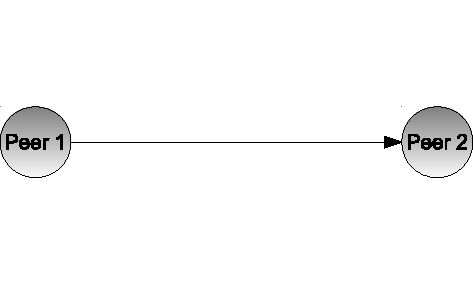
\includegraphics[width=\textwidth]{img/mep_arch_unicast.pdf}
\caption{Unicast}
\label{fig:mep_arch_unicast} 
\end{minipage}
}
\hfill
\fbox{
\begin{minipage}[t]{0.43\textwidth}

\paragraph{Multicast}
\begin{itemize}
\item Message: n  
\item Confirmation (optional): n
\end{itemize}

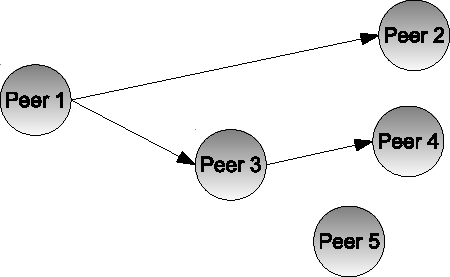
\includegraphics[width=\textwidth]{img/mep_arch_multicast.pdf}
\caption{Multicast}
\label{fig:mep_arch_multicast} 
\end{minipage}
}
\end{figure}

%\subsection*{One-way:}
%\paragraph{Unicast}
%\begin{itemize}
%\item Request: 1 
%\item Confirmation (optional): 1
%\end{itemize}
%\myfig[8 cm]{mep_arch_unicast}{Unicast}
%
%
%
%\paragraph{Multicast}
%\begin{itemize}
%\item Request: n  
%\item Confirmation (optional): n
%\end{itemize}
%\myfig[8 cm]{mep_arch_multicast}{Multicast}
%
%\pagebreak

%\pagebreak

\subsection*{Request-Response:}

%\subsection*{Request-Response:}
%\paragraph{SingleRequestSingleResponse}
%\begin{itemize}
%\item Request: 1  
%\item Response: 1
%\end{itemize}
%\myfig[8 cm]{mep_arch_srsr}{SingleRequestSingleResponse}
%
%\paragraph{SingleRequestMultiResponse}
%\begin{itemize}
%\item Request: 1  
%\item Response: n
%\end{itemize}
%\myfig[8 cm]{mep_arch_srmr}{SingleRequestMultiResponse}

\paragraph{Single Request Single Response}
Eine Single Request Single Response Nachricht entspricht einer Unicast Nachricht, die {\it eine} Antwort zur"uckgeschickt. Diese Antwort enth"alt ebenfalls einen Inhalt.
\paragraph{Single Request Multi Response}
Eine SingleRequestMultiResponse Nachricht entspricht einer Unicast Nachricht, die {\it mehrere} Antworten zur"uckgeschickt. Diese Antworten enthalten ebenfalls jeweils einen Inhalt.
\paragraph{Multi Request Multi Response}
Eine MultiRequestMultiResponse Nachricht entspricht einer Multicast Nachricht, die {\it jeweils eine oder mehrere} Antworten zur"uckgeschickt. Diese Antworten enthalten ebenfalls jeweils einen Inhalt.

\clearpage

\begin{figure}[htbp]
\fbox{
\begin{minipage}[t]{0.43\textwidth}
	
\paragraph{Single Request Single Response}
\begin{itemize}
\item Request: 1 
\item Response: 1
\end{itemize}


\includegraphics[width=\textwidth]{img/mep_arch_srsr.pdf}
\caption{Single Request $ $ $ $ $ $ $ $ Single Response}
\label{fig:mep_arch_srsr} 
\end{minipage}
}
\hfill
\fbox{

\begin{minipage}[t]{0.43\textwidth}
\paragraph{Single Request Multi Response}
\begin{itemize}
\item Request: 1  
\item Response: 1..n
\end{itemize}


\includegraphics[width=\textwidth]{img/mep_arch_srmr.pdf}
\caption{Single Request $ $ $ $ $ $ $ $ $ $ Multi Response}
\label{fig:mep_arch_srmr} 
\end{minipage}
}
\end{figure}

\begin{figure}[!h]
\begin{center}
\fbox{
	\begin{minipage}[t]{0.42\textwidth}
	
\paragraph{Multi Request Multi Response}
\begin{itemize}
\item Request: 1..n 
\item Response: 1..m
\end{itemize}

	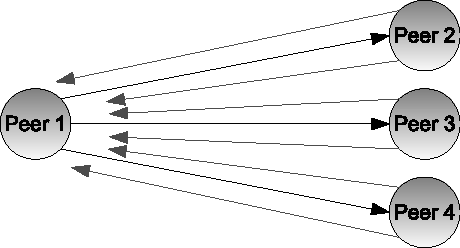
\includegraphics[width=\textwidth]{img/mep_arch_mrmr.pdf}
	\caption{Multi Request $ $ $ $ $ $ $ $ Multi Response}
	\label{fig:mep_arch_mrmr} 
	\end{minipage}
	}
	\end{center}
\end{figure}

%\paragraph{MultiRequestMultiResponse}
%\begin{itemize}
%\item Request: n  
%\item Response: n
%\end{itemize}
%\myfig[8 cm]{mep_arch_mrmr}{MultiRequestMultiResponse}



Aus der oben beschriebenen Definition kann nun, mittels der Unterscheidung zwischen {\it Unreliable} (Anfrage ohne Best"atigung bzw. Antwort) und {\it Reliable} (Anfrage mit Best"atigung bzw. Antwort), das folgende komplette Pattern abgleitet werden:

\begin{itemize}
\item Unreliable Messaging
\begin{itemize}
\item Unreliable Unicast
\item Unreliable Multicast
\end{itemize}
\item Reliable Messaging
\begin{itemize}
\item Reliable Unicast
\item Reliable Multicast
\item Single Request Single Response
\item Single Request Multi Response
\item Multi Request Multi Response
\end{itemize}
\end{itemize}

\subsubsection{Anmerkung}
Bei der Betrachtung der oben beschriebenen Definition k"onnte nun die Frage aufkommen, warum hier zwischen dem {\it Unreliable} und {\it Reliable} Messaging (z.B. bei Unicast-Nachrichten) unterschieden wird. Bei jedem Nachrichtenversand eines Reliable Messaging Pattern wird jeweils eine Best"atigung bzw. Antwort zum Sender zur"uckgeschickt. Dieses bedeutet allerdings sowohl einen zus"atzlichen Netzwerkverkehr als auch eine zus"atzliche Wartezeit auf die Antwort, obwohl diese gegebenfalls gar nicht ben"otigt wird.

\section{Architektur}
\label{sec:architektur}
Wie bereits erw"ahnt setzt diese Bachelorarbeit auf dem Netty-Framework (Abschnitt \ref{sec:netty}) auf. Dementsprechend orientiert sich die gew"ahlte Architektur an diesem Framework. Die Architektur setzt sich dabei aus der Channel-Architektur und der Pipeline-Architektur zusammen.

\subsection{Aufbau}
\label{subsec:mep-arch-channel}

Die gew"ahlte Channel-Architektur ist aus den folgenden Komponenten zusammengesetzt:

\begin{itemize}
\item {\bf Unicast / Multicast Channel}: wird einzig zum Versenden von Unicast und Multicast Nachrichten verwendet.
\item {\bf Single Request Single Response Channel}: wird einzig zum Versenden von Single Request Single Response Nachrichten verwendet.
\item {\bf Multi Response Channel}: wird einzig zum Versenden von Multi Response Nachrichten, namentlich Single Request Multi Response und Multi Request Multi Response verwendet.
\item {\bf RPC Channel}: wird einzig zum Aufruf von Remote Procedure Calls verwendet.
\end{itemize}

\myfig{mep-channel-arch}{Vereinfachte Channel-Architektur}

Die Zusammensetzung der einzelnen Komponenten ist in Abbildung \ref{fig:mep-channel-arch} veranschaulicht, dabei ist die Transportschicht durch das Uberlay-Projekt (Abschnitt \ref{sec:uberlay}) gegeben. Die Channel sind mittels einer Multiplexer / Demultiplexer -Logik, mit der Transportschicht verbunden. Jeder Channel besitzt eine eigene Pipeline, die wiederum Handler enth"alt, die f"ur die Verarbeitung der Nachrichten sorgen. 

\subsection{Erl"auterung}
Die gew"ahlte Architektur, welche oben beschrieben ist,orientiert sich an dem Aufbau der Netty-Architektur. Unicast bzw. Multicast Nachrichten liefern Confirmations zur"uck, die keinen Payload enthalten. Responses des Request-Response-Pattern, namentlich Single Request Single Response, Single Request Multi Response und Multi Request Multi Response liefern Responses zur"uck, welche mittels eigener ChannelFuture-Objekte, erzeugt werden. Der RPC Channel wiederum erm"oglicht die Benutzung von Protobuf (Abschnitt \ref{sec:google-protobuf}).

%\subsection{Pipeline-Architektur}
%\label{subsec:mep-arch-pipeline}
%Jeder Peer besitzt einen Socket, welcher wie bereits in Kapitel \ref{sec:netty} beschrieben, eine Pipeline, namentlich {\bf ChannelPipeline} enth"alt. Desweiteren enth"alt jeder Peer zus"atzlich noch eine {\bf SingleRequestSingleResponseChannelPipeline} sowie eine {\bf MultiResponseChannelPipeline}. Die Abbildung \ref{fig:mep_arch} zeigt dabei die daraus resultierende Ubermep-Architektur inklusive der Anbindung an das Uberlay-Modul. 
%
%%\myfig[10 cm]{mep_arch}{Ubermep-Pipeline-Architektur mit Anbindung an Uberlay}
%
%Zentraler Einstiegspunkt der Ubermep-Architektur ist der {\bf Peer} welche die {\bf ApplicationChannelPipeline} bereith"alt. Desweiteren verbindet der {\bf Peer} die ApplicationChannelPipeline mit der {\bf SingleRequestSingleResponseChannelPipeline} sowie der {\bf MultiResponseChannelPipeline}. 
%
%Die verschiedenen ChannelPipelines sind dabei wie folgt aufgebaut:
%
%\subsubsection{ApplicationChannelPipeline}
%
%%\myfig[6 cm] {mep-channel-pipeline-arch-a}{Aufbau der ApplicationChannelPipeline}
%
%Die ApplicationChannelPipeline wird dem Uberlay-Module "ubergeben (siehe \ref{sec:uberlay}). Die Handler bzw. Enkoder und Dekoder besitzen dabei die folgenden Aufgaben (von unten nach oben):
%\begin{itemize}
%\item Auf der untersten Ebene befinden sich der {\bf ProtobufEncoder} und {\bf ProtobufDecoder} zum verarbeiten der serialisierten Protobuf-Protokoll-Nachrichten. 
%\item Dar"uber befindet sich der {\bf UnreliableServiceHandler}, verantworlich f"ur die Unreliable Unicast bzw. Unreliable Multicast Nachrichten. 
%\item Dar"uber verarbeitet der {\bf ReliableServiceHandler} die Reliable Nachrichten namentlich Reliable Unicast bzw. Reliable Multicast. Desweiteren besitzt der ReliableServiceHandler den Einstiegspunkt zum Versenden von SingleRequestSingleResponse, SingleRequestMultiResponse und MultiRequestMultiResponse Nachrichten. Diese werden dann an die jeweils zust"andige Pipeline weitergeleitet.
%\item Dar"uber befinden sich s"amtliche manuell am jeweiligen Peer zus"atzlich hinzugef"ugten ServiceHandler (in der Abbildung als AdditionalServiceHandler gekennzeichnet).   Der Benutzer wiederum bestimmt dabei selber die Reihenfolge bei mehrfach hinzugef"ugten ServiceHandlern. 
%\item Ganz oben in der Pipeline befindet sich dann der {\bf RpcServiceHandler} der sich f"ur die Remote Procedure Calls verantworlich zeichnet.
%\end{itemize}
%
%Die nun folgenden Request-Response-Pattern (s. Abschnitt \ref{sec:architektur}) zugeh"origen Pipelines und deren Handler sorgen beim Senden f"ur die Umwandlung in serialisierbare Protokoll-Nachrichten bzw. beim Empfangen f"ur die Umwandlung der serialisierten Protokoll-Nachrichten in ein Objekt des entsprechenden Nachrichtentyps des Message Exchange Patterns.
%
%\subsubsection{SingleRequestSingleResponseChannelPipeline}
%
%%\myfig[9 cm]{mep-channel-pipeline-arch-b}{Aufbau der SingleRequestSingleResponseChannelPipeline}
%
%In der SingleRequestSingelResponsePipeline werden ausschlie"slich die Single\-Request\-Single\-Response-Nachrichten verarbeitet. Sie besitzt nur einen Handler mit der folgenden Aufgabe:
%\begin{itemize}
%\item Der {\bf SingleRequestSingleResponseServiceHandler} verarbeitet den Versand und Empfang von SingleRequestSingleResponse-Nachrichten. 
%\end{itemize}
%
%\subsubsection{MultiResponseChannelPipeline}
%
%%\myfig[7 cm]{mep-channel-pipeline-arch-c}{Aufbau der MultiResponseChannelPipeline}
%
%In der MultiResponseChannelPipeline werden ausschlie"slich die MultiResponse-Nachrichten, namentlich SingleRequestMultiResponse bzw. MultiRequestMultiResponse verarbeitet. Sie besitzt zwei Handler mit den folgenden Aufgaben:
%\begin{itemize}
%\item Auf der untersten Ebene befindet sich der {\bf SingleRequestMultiResponseServiceHandler}, der den Versand und Empfang von Single\-Request\-Multi\-Response-Nachrichten verarbeitet.
%\item Dar"uber befindet sich der {\bf MultiRequestMultiResponseServiceHandler}, der den Versand und Empfang von MultiRequestMultiResponse-Nachrichten verarbeitet.
%\end{itemize}
%
%\subsection{Ubermep-Architektur}
%Der nun folgende Abschnitt beschreibt das Zusammenspiel zwischen der in Abschnitt \ref{subsec:mep-arch-channel} beschriebenen Channel-Architektur und der in Abschnitt \ref{subsec:mep-arch-pipeline} beschriebenen Pipeline-Architektur.
%
%\subsubsection{ApplicationChannel und ApplicationChannelPipeline}
%Die ApplicationChannelPipeline wird nun auf den ApplicationChannel aufgesetzt welcher zwischen dem Sender-Socket und Empf"anger-Socket aufgebaut wird. Die Anbindung der ApplicationChannelPipeline an den ApplicationChannel ist in Abbildung \ref{fig:mep-app_channel-arch} verdeutlicht. Die Abbildung soll dabei das Senden einer Nachricht des {\it One-way} -Pattern veranschaulichen. Die rechte Seite der ApplicationPipeline entspricht der ApplicationPipeline Sender-seitig, die linke Seite der ApplicationPipeline Empf"anger-seitig. Anmerkung: In der Abbildung \ref{fig:mep-app_channel-arch} sind einige ServiceHandler der ApplicationPipeline weggelassen worden, um das Schaubild nicht "ubersichtlich zu halten. Die ApplicationPipeline eines Peers, entspricht {\it immer} der, in Abschnitt \ref{subsec:mep-arch-pipeline} beschriebenen Form. 
%
%Der Ablauf beim Versenden einer One-way-Pattern-Nachricht ist nun wie folgt:
%\begin{itemize}
%\item Am Client (Peer 1) wird das Nachrichten-Objekt des One-way Pattern downstream in der ApplicationChannelPipeline weitergereicht bis der entsprechende ServiceHandler die Nachricht in eine Protokoll-Nachricht umwandelt. 
%\item Diese wird dann mittels des ProtobufEncoder serialisiert
%\item und "uber den ApplicationChannel an den Server (Peer 2) gesendet.
%\item Dort wird dann die serialisierte Nachricht mittels des ProtobufDecoder in eine Protokoll-Nachricht deserialisiert 
%\item und upstream an den entsprechenden ServiceHandler weitergereicht.
%\item Der ServiceHandler wandelt diese Nachricht dann in das entsprechende Nachrichten-Objekt um.
%\end{itemize}
%
%\myfig{mep-app_channel-arch}{Vereinfachte ApplicationChannel und -Pipeline Architektur}
%
%\subsubsection{SingleRequestSingleResponseChannel und SingleRequestSingleResponseChannelPipeline}
%Wie bereits in Abschnitt \ref{subsec:mep-arch-channel} beschrieben ist der SingleRequestSingleResponseChannel mittels einer Multiplexer / Demultiplexer -Logik mit dem ApplicationChannel verbunden. Zus"atzlich ist der SingleRequestSingleResponseChannel Client-seitig sowie Server-seitig mit einer SingleRequestSingleResponseChannelPipeline verbunden. Im folgenden soll nun anhand des Versenden bzw. Empfangen einer SingleRequestSingleResponse-Nachricht das Zusammenspiel der verschiedenen Channels sowie Pipelines verdeutlicht werden. Die Abbildung \ref{fig:mep-srsr_channel-arch} veranschaulicht dabei diesen Ablauf.
%
%\myfig{mep-srsr_channel-arch}{Vereinfachte SingleRequestSingleResponse-Ubermep Architektur}
%
%\begin{itemize}
%\item (1) Der SingleRequestSingleResponseChannel hat beim Versenden einer Single\-Request\-SingleResponse-Nachricht seinen Einstiegspunkt im {\bf ReliableServiceHandler}. 
%\item (2) Dieser (ReliableServiceHandler) leitet diese dann an den SingleRequestSingleResponseChannel weiter und 
%\item (3) der zugeh"orige SingleRequestSingleResponseServiceHandler baut diese Nachricht in eine Protokoll-Nachricht (siehe Abschnitt \ref{sec:protokoll}) um. 
%\item (4) Die ChannelSink leitet diese Protokoll-Nachricht 
%\item (5) dann an den ApplicationChannel weiter. 
%\item (6) Diese wird dann vom ProtobufEncoder encodiert und an den Remote-Peer gesendet. 
%\item (7) Der ReliableServiceHandler des Remote-Hosts bekommt dann diese Nachricht hochgereicht. 
%\item (8) Der SingleRequestSingleResponseServiceHandler empf"angt dann den Protokoll-Nachricht-Request, baut daraus eine Protokoll-Response-Nachricht und 
%\item gibt diese zur"uck and den ReliableServiceHandler. Dieser sendet dann diese Protokoll-Response-Nachricht downstream zur"uck zum Sender. 
%\item Der Sender empf"angt diese Response upstream im ReliableServiceHandler 
%\item und leitet diese an den SingleRequestSingleResponseChannel weiter, 
%\item so dass diese Protokoll-Nachricht im SingleRequestSingleResponseServiceHandler in eine SingleRequestSingle\-Response-Response umgewandelt werden kann. 
%\item Diese wird dann an den ReliableServiceHandler des Senders zur"uckgegeben.
%\end{itemize}
%
%\subsubsection{MultiResponseChannel und MultiResponseChannelPipeline}
%So wie der SingleRequestSingleResponseChannel, ist auch der MultiResponseChannel, wie bereits in Abschnitt \ref{subsec:mep-arch-channel} beschrieben, mittels einer Multiplexer / Demultiplexer -Logik mit dem ApplicationChannel verbunden. Der Ablauf einer MultiResponse-Nachricht, ist dabei analog zu der einer Single\-Request\-Single\-Response-Nachricht. Im folgenden soll deshalb nur auf die Unterschiede eingangen werden, wobei die Abbildung \ref{fig:mep-mr_channel-arch} auch hierbei den Ablauf veranschaulicht:
%
%\begin{itemize}
%\item der ReliableServiceHandler leitet die Nachricht an den MultiResponseChannel weiter
%\item der MultiRequestMultiResponseChannel baut, beim Versand, die Multi\-Request\-Multi\-Response-Nachricht in eine entsprechende Protokoll-Nachricht um
%\item der SingleRequestMultiResponseChannel baut, beim Versand, die Single\-Request\-Multi\-Response-Nachricht in eine entsprechende Protokoll-Nachricht um
%\item der Empfang einer Protokoll-Nachricht im ReliableServiceHandler ist dabei analog zu der oben beschrieben Logik
%\end{itemize}
%
%\myfig{mep-mr_channel-arch}{Vereinfachte MultiResponse-Ubermep Architektur}
%
%\subsubsection{UbermepRpcChannel und ApplicationChannelPipeline}
%Wie bereits im Kapitel \ref{sec:google-protobuf} erw"ahnt setzt die genutzte {\it Remote Procedure Call} -Architektur auf Google Protobuf auf, d.h. der RPC-Channel hat nichts mit den bisherigen beschriebenen (Netty) -Channels gemein, besitzt dementsprechend auch keine entsprechende ChannelPipeline. Trotzdem hat der UbermepRpcChannel einen korrespondierenden ServiceHandler, namentlich {\it RpcServiceHandler}, welcher in der ApplicationChannelPipeline sitzt (siehe Abschnitt \ref{subsec:mep-arch-pipeline}).
%Das Zusammenspiel des UbermepRpcChannel und der ApplicationChannelPipeline soll nun anhand eines Ablaufs eines Ubermep-Remote-Procedure-Calls mit Hilfe der Abbildung \ref{fig:mep-rpc_channel-arch} veranschaulicht werden. 
%
%\myfig{mep-rpc_channel-arch}{Vereinfachte RPC-Ubermep Architektur}
%
%Der Ablauf eines Remote Procedure Calls ist dabei wie folgt, wobei im folgenden der aufrufende Peer als Client und der ausf"uhrende Peer als Server benannt ist. 
%\begin{itemize}
%\item Zuerst wird der aufzurufende Service am Server-Peer registriert (siehe dazu Abschnitt \ref{sec:rpc}).
%\item Anschlie"send wird ein UbermepRpcChannel zum Server aufgebaut.
%\item (1) F"ur diesen Channel wird ein zugeh"origer Stub generiert.
%\item "Uber diesen Stub wird dann die Methode ausgef"uhrt. 
%\item (2) Dabei wird dann "uber den UbermepRpcChannel der RpcServiceHandler aufgerufen. 
%\item (3) Dieser (RpcServiceHandler) wandelt den RPC in eine Protokoll-Nachricht um und leitet diese an den ApplicationChannel des Uberlay-Moduls weiter. 
%\item (4) Anschlie"send wird die Protokoll-Nachricht downstream an den Server-Peer verschickt. 
%\item (5) Am Server-Peer wird diese dann upstream empfangen 
%\item (6) an den RpcServiceHandler weitergereicht
%\item (7) und anschlie"send im Service ausgef"uhrt. 
%\item (8) Das Ergebnis wird dann an den RpcServiceHandler zur"uckgegeben, 
%\item und anschlie"send am Server in eine Protokoll-Antwort umgebaut, 
%\item die dann wiederum "uber den ApplicationChannel im RpcServiceHandler des aufrufenden Clients landet. 
%\item (9) Die Anwort wird schlu"sendlich "uber den UbermepRpcChannel an die aufrufende Methode zur"uckgegeben.
%\end{itemize}


\section{Protokoll}
\label{sec:protokoll}
Im Folgenden Abschnitt werden nun die, im Abschnitt \ref{sec:mep} spezifizierten Message Exchange Pattern in ein Protokoll umgewandelt. Mittels diesem Protokoll k"onnen dann Nachrichtentypen des Message Exchange Pattern "uber den entsprechenden Channel versendet werden.

\subsection{Struktur}
Dieser Abschnitt zeigt den schematischen Aufbau des verwendeten Protokolls und beschreibt deren ben"otigte und optionale Felder. In Abbildung \ref{fig:mep_protokoll} ist die Struktur des Protokolls zu sehen. Dabei sind die optionalen Felder mit * gekennzeichnet. Diese Felder werden nur "ubertragen, wenn sie ben"otigt werden. 
\myfig{mep_protokoll}{Schematischer Aufbau des Protokolls}

Die in Abbildung \ref{fig:mep_protokoll} beschriebenen Felder haben die folgende Bedeutung: 

\begin{itemize}
\item {\bf ID}: erm"oglicht die eindeutige Identifizierung einer Nachricht.
\item {\bf Typ}: besteht aus einem der folgenden m"oglichen Nachrichtentypen:
\begin{itemize}
\item UNICAST
\item MULTICAST
\item SINGLE\_RESPONSE\_REQUEST
\item MULTI\_RESPONSE\_REQUEST
\item SINGLE\_RESPONSE
\item MULTI\_RESPONSE
\item RPC\_REQUEST
\item RPC\_RESPONSE
\end{itemize}
\item Das Flag {\bf Reliable} wird gesetzt falls eine Nachricht zu dem \emph{Reliable Messaging} Pattern geh"ort.
\item {\bf Akt. Nachricht}: wird \emph{nur} f"ur MultiResponse-Nachrichten "ubertragen. Dieses Feld zeigt an welche Nummer die entsprechende Response besitzt. Beispiel: \emph{(Aktuelle Nachricht)} {\bf 2} von \emph{(Anzahl Nachrichten)} 4.
\item {\bf Anz. Nachrichten}: wird \emph{nur} f"ur MultiResponse-Nachrichten ben"otigt und beschreibt die zu erwartenden Responses. 
\item {\bf Payload}: enth"alt den zu "ubertragenen Inhalt.
\end{itemize}
%\paragraph{ID}
%Die \emph{ID} erm"oglicht die eindeutige Identifizierung einer Nachricht.

%\paragraph{Typ}
%Ein \emph{Typ} besteht aus einem der folgenden m"oglichen Nachrichtentypen:
%\begin{itemize}
%\item UNICAST
%\item MULTICAST
%\item SINGLE\_RESPONSE\_REQUEST
%\item MULTI\_RESPONSE\_REQUEST
%\item SINGLE\_RESPONSE
%\item MULTI\_RESPONSE
%\item RPC\_REQUEST
%\item RPC\_RESPONSE
%\end{itemize}

%\paragraph{Reliable}
%Das Flag \emph{Reliable} wird gesetzt falls eine Nachricht zu dem \emph{Reliable Messaging Pattern} geh"ort.

%\paragraph{Akt. Nachricht}
%Das Feld \emph{Aktuelle Nachricht} wird \emph{nur} f"ur MultiResponse-Nachrichten ben"otigt. Dieses Feld zeigt an welche Nummer die entsprechende Response besitzt. Beispiel: \emph{(Aktuelle Nachricht)} {\bf 2} von \emph{(Anzahl Nachrichten)} 4.

%\paragraph{Anz. Nachrichten}
%Das Feld \emph{Anzahl Nachrichten} beschreibt die zu erwartenden Responses und wird \emph{nur} f"ur MultiResponse-Nachrichten ben"otigt.

%\paragraph{Payload}
%Das Feld \emph{Payload} enth"alt den zu "ubertragenen Inhalt.

\subsection{Nachrichten}
Im Folgenden wird nun die oben spezifizierte Struktur auf die Nachrichtentypen des Message Exchange Pattern angewendet. Dabei wurden in der Beschreibung die Felder \emph{ID} und \emph{Payload} nicht ber"ucksichtigt, da diese auf die unterschiedlichen Nachrichtentypen keinen Einfluss haben. Desweiteren werden die Elemente \emph{x} und \emph{-} eingef"uhrt. Sie besitzen die folgende Bedeutung:

\begin{tabular}{rl}
x & := gesetzt \\
- & := nicht gesetzt \\
 \end{tabular}

\begin{figure}[h]
\subsubsection{Unreliable Messaging}

\subsubsection{\hspace{10mm} Unreliable Unicast}
\subfigure[Unreliable Unicast-Request]{
\label{fig:mep_protokoll_unrel_unicast}
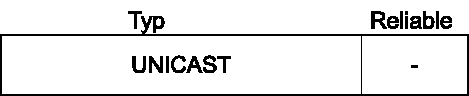
\includegraphics{img/mep_protokoll_unrel_unicast.pdf}
%\caption{UnreliableUnicast-Request}
}

\subsubsection{\hspace{10mm} Unreliable Multicast}
\subfigure[Unreliable Multicast-Request]{
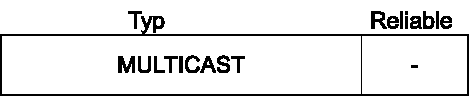
\includegraphics{img/mep_protokoll_unrel_multicast.pdf}
\label{fig:mep_protokoll_unrel_multicast} 
}
\end{figure}

\begin{figure}[h]
\subsubsection{Reliable Messaging}

\subsubsection{\hspace{10mm} Reliable Unicast}
\subfigure[Reliable Unicast-Request]{
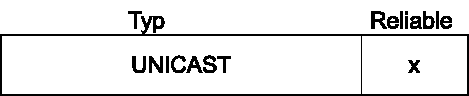
\includegraphics{img/mep_protokoll_rel_unicast.pdf}
\label{fig:mep_protokoll_rel_unicast} 
}

\subsubsection{\hspace{10mm} Reliable Multicast}
\subfigure[Reliable Multicast-Request]{
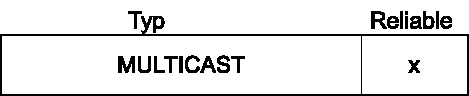
\includegraphics{img/mep_protokoll_rel_multicast.pdf}
\label{fig:mep_protokoll_rel_multicast}
}
\end{figure}

\begin{figure}[h]
\subsubsection{\hspace{10mm} Single Request Single Response}
\subfigure[Single Request Single Response-Request]{
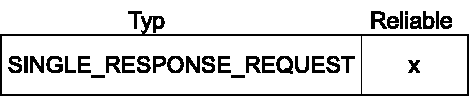
\includegraphics{img/mep_protokoll_srsr_req.pdf}
\label{fig:mep_protokoll_srsr_req} 
}

\subfigure[Single Request Single Response-Response]{
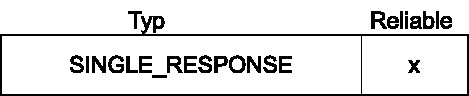
\includegraphics{img/mep_protokoll_srsr_res.pdf}
\label{fig:mep_protokoll_srsr_res}  
}
\end{figure}

\clearpage

\begin{figure}[h]
\subsubsection{\hspace{10mm} Multi Response}
Im Folgenden werden Single Request Multi Response und Multi Request Multi Response Nachrichten in einem \emph{Multi Response}-Typ zusammengefasst.
Die Unterscheidung hierbei wird "uber das Feld ID geregelt.
\subfigure[Multi Response-Request]{
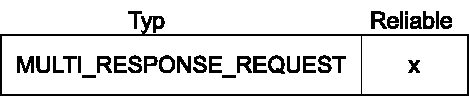
\includegraphics{img/mep_protokoll_mr_req.pdf}
\label{fig:mep_protokoll_mr_req} 
}

\subfigure[Multi Response-Response]{
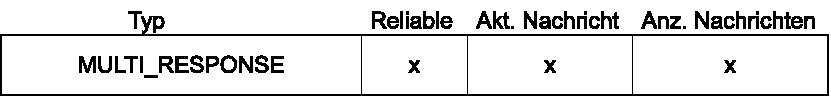
\includegraphics{img/mep_protokoll_mr_res.pdf}
\label{fig:mep_protokoll_mr_res}  
}
\end{figure}

\begin{figure}[h]
\subsubsection{Remote Procedure Call}
\subfigure[RPC-Request]{
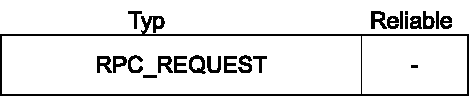
\includegraphics{img/mep_protokoll_rpc_req.pdf}
\label{fig:mep_protokoll_rpc_req} 
}

\subfigure[RPC-Response]{
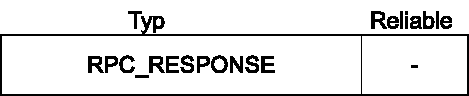
\includegraphics{img/mep_protokoll_rpc_res.pdf}
\label{fig:mep_protokoll_rpc_res}  
}
\end{figure}

	\chapter{Implementierung}
\label{cha:implementierung}

In diesem Kapitel wird die Implementierung, genannt \emph{Ubermep}, des in Kapitel \ref{cha:entwurf} vorgestellten Architekturentwurfs erl"autert.

In Abschnitt \ref{sec:einleitung} wird zun"achst ein "Uberblick "uber die Struktur der Implementierung gegeben. Danach wird erl"autert wo und wie die im Grundlagenteil in Kapitel \ref{cha:grundlagen} 
vorgestellten Technologien Anwendung finden. Anschlie"send wird das im Entwurfskapitel spezifizierte Protokoll in Abschnitt \ref{sec:impl_protokoll} sowie die entwickelte Bibliothek, also der Kern der Implementierung in Abschnitt \ref{sec:ubermep-core} genauer beleuchtet.

In Abschnitt \ref{sec:beispiele} wird dann anhand von Beispielen gezeigt, wie ein Peer-to-Peer Overlay-Netzwerk mittels der Implementierung erzeugt werden kann und wie man "uber das Netzwerk Nachrichten des Message Exchange Pattern versendet, sowie Remote Procedure Calls "uber das Netzwerk ausgef"uhrt werden.

Abschlie"send wird in Abschnitt \ref{sec:zukunft} eine Auswahl von m"oglichen zuk"unftigen Erweiterung der Implementierung vorgestellt.

\section{Einleitung und "Uberblick}
\label{sec:einleitung}

Wie bereits in Abschnitt \ref{sec:maven} erl"autert wurde diese Arbeit mittels dem Build-Tool Maven entworfen. Daraus ergibt sich eine Projektstruktur bestehend aus verschiedenen Maven-Untermodulen welche im Folgenden Abschnitt erl"autert werden. 
\subsection*{Struktur und Komponenten}

Diese Implementierung besteht aus 5 verschiedenen Untermodulen welche in einem sogenannten {\it Multi Module Project} zusammengefasst werden. Jedes Untermodul erbt von der Parent POM des {\bf Ubermep-parent} Moduls. Die Aufteilung der verschiedenen Module ist hierbei im Listing \ref{lst:ubermep-parent-dir} zu erkennen.

\lstinputlisting[language=Python,caption=Ausschnitt aus der Ubermep-parent pom.xml,label=lst:ubermep-parent-dir,firstnumber=1]{lst/ubermep-parent-dir.txt}

Im Folgenden nun eine kurze Beschreibung der einzelnen Module: 
\begin{itemize}
\item {\bf ubermep-parent} ist das Parent-Modul dieser Arbeit, welches den POM enth"alt. In seiner {\tt pom.xml} werden dabei die enthaltenen Untermodule, sowie die in den Untermodulen ben"otigten Abh"angigkeiten definiert. Diese Abh"angigkeiten werden dann an die Untermodule vererbt.
\item{\bf ubermep-cmdline} enth"alt den Einstiegspunkt zum starten der Applikation aus der Kommandozeile. 
\item{\bf ubermep-core} enth"alt die Bibliothek von ubermep. Dieses Modul h"alt unter anderem das zentrale Interface {\bf Peer} bereit, welches ben"otigt wird um ein Overlay-Netzwerk zu erzeugen und Nachrichten des Message Exchange Pattern auszutauschen. Dieses Modul wird in Abschnitt \ref{sec:ubermep-core} detailiert erkl"art.
\item{\bf ubermep-example} enth"alt Beispiel-Anwendungen wie ubermep-core genutzt werden kann. 
\item{\bf ubermep-gui} enth"alt eine Grafische Oberfl"ache zum Erzeugen eines Overlay-Netzwerks sowie zum Senden von Nachrichten des Message Exchange Pattern.
\end{itemize}
Da nur das Modul {\bf Ubermep-core} die Bibliothek von ubermep enth"alt, wird in diesem Kapitel, in Abschnitt \ref{sec:ubermep-core} auch nur auf dieses Modul n"aher eingegangen. Im Folgenden aber zun"achst die Implementierung des in Abschnitt \ref{sec:protokoll} vorgestellten Protokolls.

% <----- START Protokoll

\section{Protokoll}
\label{sec:impl_protokoll}
Wie im Abschnitt \ref{sec:google-protobuf} bereits erl"autert, wird zum Generieren der Protokoll-Nachrichten Google-Protobuf verwendet. Im Listing \ref{lst:meppacket} ist die mittels der Protobuf-IDL erstellten Protokoll-Datei zu erkennen, die auf der Spezifikation des Protokoll-Entwurfs (\ref{sec:protokoll}) des Entwurfskapitel 3 basiert. Diese kann dann unter Benutzung des Protobuf-Compiler als serialisierte Protokoll-Nachricht "uber den Kommunikationskanal versendet werden.

\subsubsection{MEPPacket}
Das serialisierbare Protokoll dieser Applikation, das {\it MEPPacket}, ist wie folgt aufgebaut:

\lstset{caption=MEP.proto,label=lst:meppacket}
\begin{lstlisting}
message MEPPacket {
    required bool reliable = 1;
    required MessageType messageType = 2;
    required bytes payload = 3;
    
    optional uint32 requestID = 4;
    optional bool exceptionOccurred = 5;
    optional uint32 currentMessageNumber = 6;
    optional uint32 totalMessageNumber = 7;
    optional RPCMessage rpcMessage = 8;
}
\end{lstlisting} 

Es besteht aus den ben"otigten {\it (required)} Feldern: 
\begin{itemize}
\item {\bf reliable} spezifiziert ob eine Unicast bzw. Multicast-Nachricht {\it reliable} und {unreliable} ist. Request-Response-Nachrichten sind immer {\it reliable}
\item {\bf messageType} beschreibt den Pattern - Typ der Nachricht. Eine genauere Beschreibung findet sich weiter unten.
\item {\bf payload} enth"alt den Inhalt einer Nachricht
\end{itemize}
sowie den optionalen {\it (optional)} Feldern, die nur "ubertragen werden, wenn ben"otigt:
\begin{itemize}
\item {\bf requestID} wird intern f"ur die Abarbeitung von Request-Response-Nachrichten ben"otigt. Jeder Request bekommt beim Aufruf eine RequestID zugewiesen. Wird die "uber die RequestID gekennzeichnete korrespondierende Response empfangen, so wird der Request als erfolgreich ausgeliefert gewertet.
\item {\bf exceptionOccured} zeigt an ob Server-seitig, also auf der Seite des Empf"angers, beim Abarbeiten des {\it payloads} eine Ausnahme aufgetreten ist
\item {\bf currentMessageNumber} zeigt an, welche Nummer die Antwort besitzt. Dieses Feld wird ausschlie"slich f"ur MultiResponse-Nachrichten ben"otigt
\item {\bf totalMessageNumber} zeigt an, wieviel Antworten versendet bzw. erwartet werden. Dieses Feld wird ausschlie"slich f"ur MultiResponse-Nachrichten ben"otigt
\item {\bf rpcMessage} beschreibt eine RPC-Message. Eine genauere Erl"auterung findet sich weiter unten.
\end{itemize}

\paragraph{MessageType}
Der Aufz"ahlungstyp {\it MessageType} spezifiziert den Pattern -Typ der Nachricht und ist wie folgt aufgebaut: 

\lstset{firstnumber=12, label=lst:messageType}
\begin{lstlisting}
enum MessageType {
    UNICAST = 1;
    MULTICAST = 2;
    SINGLE_RESPONSE_REQUEST = 3;
    MULTI_RESPONSE_REQUEST = 4;
    SINGLE_RESPONSE = 5;
    MULTI_RESPONSE = 6;
    RPC_REQUEST = 7;
    RPC_RESPONSE = 8;
}
\end{lstlisting}
Der MessageType enth"alt die folgenden Nachrichten-Typen:
\begin{itemize}
\item {\bf UNICAST} ist zust"andig f"ur Unicast Nachrichten; hierbei findet keine Unterscheidung zwischen unreliable bzw. reliable Unicast statt. Dies wird "uber das Flag {\bf reliable} im {\bf MEPPacket} spezifiziert
\item {\bf MULTICAST} ist zust"andig f"ur Multicast Nachrichten; auch hierbei findet keine Unterscheidung zwischen unreliable bzw. reliable Multicast statt.
\item {\bf SINGLE\_RESPONSE\_REQUEST} beschreibt einen Single\-Request\-Single\-Response-\-Request
\item {\bf MULTI\_RESPONSE\_REQUEST} beschreibt einen Single\-Request\-Multi\-Response-\-Request sowie f"ur ein Multi\-Request\-Multi\-Response-\-Request
\item {\bf SINGLE\_RESPONSE} ist zust"andig f"ur einen Single\-Request\-Single\-Response-\-Response
\item {\bf MULTI\_RESPONSE} ist zust"andig f"ur einen SingleRequestMultiResponse-Response sowie f"ur einen MultiRequestMultiResponse-Response
\item {\bf RPC\_REQUEST} beschreibt einen RPC-Request
\item {\bf RPC\_RESPONSE} beschreibt einen RPC-Response
\end{itemize}

\paragraph{RPCMessage}
Die {\bf RpcMessage} wird, wie oben bereits erw"ahnt f"ur den Aufruf eines Remote Procedure Calls ben"otigt und ist we folgt aufgebaut:

\lstset{firstnumber=22, label=lst:rpcMessage}
\begin{lstlisting}
message RPCMessage {
    required string serviceName = 1;
    required string methodName = 2;
    required ServiceType serviceType = 3;
}
\end{lstlisting}

Der {\it RpcMessage}-Typ besteht aus den ben"otigten {\it (required)} Feldern: 
\begin{itemize}
\item {\bf serviceName} enth"alt den Klassen-Namen des aufzurufenden RPC-Services 
\item {\bf methodName} enth"alt den Methoden-Name des aufzurufenden RPC-Services 
\item {\bf serviceType} beschreibt den Typ des aufzurufenden Service. Eine genauere Beschreibung findet sich weiter unten.
\end{itemize}
Da die Parameter mittels des eigens generierten Protobuf-RPC-Requests "ubergeben werden (siehe Abschnitt \ref{sec:google-protobuf}), brauchen diese nicht in der Protokoll-Nachricht zu "ubertragen werden.

\paragraph{ServiceType}
In ubermep wird zwischen einem blockierendem und nicht-blockierendem RPC-Aufruf unterschieden. Aus diesem Grund muss der {\bf ServiceType} f"ur die Beschreibung des {\it RpcMessage}-Typ "ubertragen werden. Dieser ist wie folgt aufgebaut:
\lstset{firstnumber=27, label=lst:serviceType}
\begin{lstlisting}
enum ServiceType {
    SERVICE = 1;
    BLOCKING_SERVICE = 2;
}

\end{lstlisting}
Der {\it ServiceType} besteht aus den Feldern: 
\begin{itemize}
\item {\bf SERVICE} wird gesetzt wenn der RPC-Service als nicht-blockierender Aufruf verwendet wird
\item {\bf BLOCKING\_SERVICE} wird gesetzt wenn der RPC-Service als blockierender Aufruf verwendet wird
\end{itemize}

% <----- END Protokoll

\section{Ubermep-core}
\label{sec:ubermep-core}

Das Modul {\bf Ubermep-core} enth"alt zum Einen das oben beschrieben Protokoll, als auch wie bereits erw"ahnt die Kernimplementierung dieser Arbeit. Es enth"alt das Interface {\bf Peer} zum Erzeugen von Peers, mit welchem dann der Aufbau eines Peer-to-Peer Overlay-Netzwerks m"oglich ist. "Uber dieses Netzwerk kann man dann Nachrichten von einem Peer zu einem weiteren Peer, bzw. mehreren weiteren Peers senden. Des weiteren ist es m"oglich "uber einen Peer einen Remote Procedure Call (siehe Abschnitt \ref{sec:rpc}) auf einem anderen Peer des Overlay-Netzwerks auszuf"uhren. Im Folgenden wird nun erl"autert, wie die Struktur des Moduls {\bf Ubermep-core} aufgebaut ist  

\subsection{Einleitung}
Im Folgenden werden zun"achst die Aufgaben eines Peers in ubermep beschrieben.

Ein Peer in ubermep besitzt die Aufgabe, ein Overlay-Netzwerk zu erzeugen oder sich mit einem bestehenden Netzwerk zu verbinden bzw. ggf. sich von diesem zu trennen Hierf"ur   wird die M"oglichkeit des Startens und Stoppens eines Peers ben"otigt. Des weiteren wird neben dem Senden von unterst"utzten Nachrichtentypen des Message Exchange Pattern, die M"oglichkeit zum Verarbeiten von empfangenden Nachrichteninhalten ben"otigt. Abschlie"send ist das Ausf"uhren von Remote-Procedure Calls sowie des Hinzuf"ugen von zus"atzlichen Handlern zum Verarbeiten von eigenen Nachrichtentypen erforderlich.

\subsection{Schnittstellen}
Im Folgenden nun die entscheidenden Schnittstellen des Ubermep-core Moduls, welche die oben beschriebenen Aufgaben definieren. Anschlie"send folgen die entsprechenden Implementierung der Schnittstellen sowie die Abh"angigkeiten der Schnittstellen untereinander. 

\subsubsection{Peer}

\myfig[85 mm]{Interfaces_Peer}{Aufbau des Peer-Interface}

Aus der Beschreibung zum Erzeugen, Verbinden bzw. Trennen eines Peers ergibt sich nun die folgende Schnittstelle:
\begin{itemize}
\item {\it getLocalUPAddress()} gibt die lokale UPAddresse zur"uck, welche die eindeutige Addressierung f"ur Nachrichten in einem Overlay-Netzwerk erm"oglicht. Sie ist vom Typ {\bf UPAddress}, kommt aus dem Uberlay-Projekt (\ref {sec:uberlay}) und ist eine Unterklasse vom Typ {\bf SocketAddress} aus dem Package {\it java.net}. Die typische Addressierung in einem Peer-to-Peer Overlay-Netzwerk erfolgt dabei z.B. "uber eine {\bf URN} (Uniform Resource Name), welche wie folgt aufgebaut ist: {\it urn:namensraum:id}, also z.B. {\it urn:itm:1} f"ur den ersten Knoten im itm-Namensraum. 
\item {\it getLocalSocketAddress()} gibt die lokale SocketAddresse zur"uck. Sie ist vom Typ {\bf InetSocketAddress} aus dem Package java.net, enth"alt einen {\it hostname}, typischerweise eine IPv4 oder eine IPv6 Adresse und einen Port. An diese lokale SocketAddresse wird dann der Netty-Channel zum Nachrichtenaustausch gebunden.
\item {\it getRemoteSocketAddress()} gibt die remote SocketAddresse vom Typ {\bf InetSocketAddress} zur"uck, mit welcher der Peer beim Start verbunden wurde. 
\item {\it connect(InetSocketAddress remoteAddress)} verbindet den Peer mit einem weiteren Peer welcher zu der "ubergebenen {\it remoteAddress} geh"ort.
\end{itemize}

\nomenclature{URN}{Uniform Resource Name}

Die weiteren Aufgaben eines Peers in ubermep sind nun in den folgenden Service-Interfaces definiert.

\subsubsection{Service}

\myfig[25 mm]{Interfaces_Service}{Aufbau des Service-Interface}
Die Aufgaben eines Services sind:
\begin{itemize}
\item {\it start()} startet einen Peer und erzeugt bzw. verbindet diesen mit einem Netzwerk.
\item {\it stop()} stoppt einen Peer und trennt diesen vom Netzwerk
\end{itemize}

\subsubsection{UbermepService}
Der UbermepService hat die Aufgabe eigene hinzugef"ugte Nachrichtentypen zu unterst"utzen.

\myfig{Interfaces_UbermepService}{Aufbau des UbermepService-Interface}

\paragraph{Unterst"utzung eigener Nachrichtentypen}
F"ur die Unterst"utzung von eigens Hinzugef"ugten Nachrichtentypen sind die folgenden Methoden von Bedeutung:
\begin{itemize}
\item {\it registerChannelHandler(SimpleChannelHandler handler)} f"ugt einen SimpleChannelHandler (aus dem Netty-Framework \ref{sec:netty}) an einem Peer hinzu. SimpleChannelHandler k"onnen sowohl empfangende, als auch gesendete Nachrichten verarbeiten.
\item {\it registerUpstreamHandler(ChannelUpstreamHandler handler)} f"ugt einen ChannelUpstreamHandler (aus dem Netty-Framework \ref{sec:netty}) an einem Peer hinzu. ChannelUpstreamHandler sind einzig f"ur das Verarbeiten von Empfangenden Nachrichten zust"andig.
\item {\it registerDownstreamHandler(ChannelDownstreamHandler handler)} f"ugt einen ChannelDownstreamHandler (aus dem Netty-Framework \ref{sec:netty}) an einem Peer hinzu. ChannelDownstreamHandler sind einzig f"ur das Verarbeiten von Gesendeten Nachrichten zust"andig.
\end{itemize}
F"ur das Nutzen von eigenen Nachrichtentypen m"u"sen dann eigene entsprechend Handler implementiert und an einem Peer mittels der entsprechenden {\it register}-Methode registriert werden. In den eigens implementierten ChannelHandlern m"ussen die jeweiligen zust"andigen Methoden "uberschrieben bzw. implementiert werden. Diese ChannelHandler werden der ChannelPipeline der entsprechenden Peers gem"a"s der Architektur des Netty-Frameworks hinzugef"ugt.

F"ur die Implementierung gibt es dabei drei verschiedene Varianten, wobei aber jeweils immer f"ur das Verarbeiten von Empfangenden Nachrichten die Methode 
{\it handleUpstream(ChannelHandlerContext ctx, ChannelEvent e)}, sowie f"urs Verarbeiten von Versendeten Nachrichten die Methode {\it handleDownstream(Channel\-HandlerContext ctx, ChannelEvent e)} "uberschrieben werden muss:
\begin{itemize}
\item {\bf Variante 1}: Umbau einer Empfangenden / Gesendeten Nachricht in einen unterst"utzten Nachrichtentyp des Message Exchange Pattern wie z.B. in eine SingleRequestSingleResponse-Nachricht.
\item {\bf Variante 2}: Hinzuf"ugen von eigenen oder mitgelieferten Netty- Decodern bzw. Encodern (\ref{sec:netty})
\item {\bf Variante 3}: Hinzuf"ugen von eigenen Protokoll-Nachrichten mittels des Google-Protobuf Projekts (\ref{sec:google-protobuf}). Zus"atzlich muss dann ein ProtobufDecoder f"ur die entsprechende Protokoll-Nachricht der Pipeline hinzugef"ugt werden. 
\end{itemize}

Anschliessend k"onnen dann diese Nachrichten mittels der folgenden Methoden versendet werden: 
\begin{itemize}
\item {\it write (Object object, UPAddress urn)} versendet eine {\it One-way} -Pattern-Nachricht an einen Empf"anger
\item {\it write(Object object, UPAddress urn, Class channelFutureClass)} versendet eine {\it Request-Response} -Pattern-Nachricht und bekommt eine Antwort mittels der als Parameter "ubergebenen ChannelFuture-Klasse zur"uck. Die "ubergegebene ChannelFuture-Klasse muss eine Implementierung der Abstrakten Klasse {\bf UbermepAbstractChannelFuture} aus dem Package {\it mep.channel.future} sein. Wobei einzig und allein der Konstruktur implementiert werden muss.
\end{itemize}
Ein Beispiel f"ur das Versenden eines eigens hinzugef"ugten Nachrichtentyp mittels Variante 1 ist im Abschnitt \ref{sec:beispiele} zu finden.

\subsubsection{UbermepUnreliableService}
\myfig[70 mm]{Interfaces_UbermepUnreliableService}{Aufbau des UbermepUnreliableService-Interface}
Die Aufgabe des UbemepUnreliableService liegt in der Versendung von Unreliable Nachrichten (siehe Kapitel \ref{sec:mep} ) und haben dementsprechend nur die eine Methode:
\begin{itemize}
\item {\it send(UnreliableRequest request)} versendet einen UnreliableRequest.
\end{itemize}

\subsubsection{UbermepReliableService}
\myfig[100 mm]{Interfaces_UbermepReliableService}{Aufbau des UbermepReliableService-Interface}
Die Aufgabe des UbermepReliableService liegt in der Versendung von Reliable Nachrichten (siehe Kapitel \ref{sec:mep}) und haben dementsprechend nur die eine Methode:
\begin{itemize}
\item {\it send(ReliableRequest request)} versendet einen ReliableRequest und gibt den Response als ListenableFuture-Objekt zur"uck.
\end{itemize}

\subsubsection{UbermepRpcService}
\myfig[95 mm]{Interfaces_UbermepRpcService}{Aufbau des UbermepRpcService-Interface}
Die Aufgabe des UbermepRpcService liegt in der Verarbeitung von Remote Procedure Calls (RPC). F"ur das Ausf"uhren von RPC's sind dabei die folgenden Methoden von Bedeutung:
\begin{itemize}
\item {\it getRpcChannel(UPAddress urn)} erzeugt einen RpcChannel zu einer Addresse eines Peers des Overlay-Netzwerk
\item {\it registerService(RpcService service)} registriert einen RpcService an einem Peer, so dass dieser von anderen Peers aufgerufen werden kann
\item {\it registerBlockingService(RpcBlockingService service)} registriert einen RpcBlockingService an einem Peer zum Ausf"uhren eines RPC
\end{itemize}
Der Ablauf ist dabei wie folgt: zuerst registriert man einen RpcService an einem Peer. Anschliessend l"asst man sich einen RpcChannel zu einer Addresse eines Peers erzeugen. "Uber diesen Channel kann man dann einen RPC ausf"uhren. Der Unterschied zwischen einem (Non-Blocking) RpcService und einem RpcBlockingService ist der, das ein RpcService ein nicht-blockierender Aufruf ist, welcher den R"uckgabewert in einem RpcCallback zur"uckgibt, w"ahrrend der RpcBlockingService ein blockierender Aufruf ist der den R"uckgabewert "uber den Methodenauruf zur"uckbekommt. 

Das Erzeugen und Aufrufen eines RPC ist im Abschnitt \ref{sec:beispiele} anhand eines Beispielaufrufes zu erkennen.

\subsubsection{RequestListenerService}
\myfig[135 mm]{Interfaces_RequestListenerService}{Aufbau des RequestListenerService-Interface}
Zum Verarbeiten von Requests werden {\it Listener} verwendet. Diese Listener werden mittels der folgenden Methoden an einem Peer registriert:
\begin{itemize}
\item {\it addRequestListener(UnicastMulticastRequestListener listener)} f"ugt ein Uni\-castMulticastRequestListener an dem jeweiligen Peer hinzu
\item{\it addRequestListener(SingleRequestSingleResponseRequestListener listener)} f"ugt ein SingleRequestSingleResponseRequestListener an dem jeweiligen Peer hinzu
\item{\it addRequestListener(MultiResponseRequestListener listener)} f"ugt ein Multi\-ResponseRequestListener an dem jeweiligen Peer hinzu
\end{itemize}

Diese Listener arbeiten dabei nach dem Pattern der {\it Chain of responsibility}. Das bedeutet die Listener eines Typs werden hintereinander in einer Kette angeordnet. Dann durchl"auft eine Anfrage die Kette. Ist ein Listener dabei, der auf die Anfrage reagiert, wird dieser verwendet und der Aufruf beendet. Wenn nicht, wird weiter nach diesem Muster die Kette abgearbeitet. Reagiert kein Listener auf die Anfrage, gilt das Verarbeiten eines Nachrichten-Inhalts als fehlgeschlagen.

Im Folgenden nun die verschiedenen Listener-Schnittstellen:

\subsubsection{UnicastMulticastRequestListener}
\myfig[135 mm]{Interfaces_UnicastMulticastRequestListener}{Aufbau des UnicastMulticastRequestListener-Interface}
\begin{itemize}
\item {\it handleUnicastMulticastRequest(String senderUrn, byte[] payload)} verarbeitet den Inhalt von Unicast und Multicast Requests. Liefert {\it true} zur"uck wenn Inhalt erfolgreich gelesen wurde, sonst {\it false}.
\end{itemize}

\subsubsection{SingleRequestSingleResponseRequestListener}
\begin{itemize}
\item {\it handleSingleRequestSingleResponseRequest(String senderUrn, byte[] requestPayload)} verarbeitet den Inhalt von SingleRequestSingleResponse-Requests. Liefert einen Response-Inhalt als {\it byte[]} zur"uck wenn Request-Inhalt erfolgreich verarbeitet wurde, sonst {\it null}. Falls bei Verarbeitung eine {\it Exception} auftritt, wird ein {\it MEPSingleResponseExceptionEvent} geworfen.
\end{itemize}

\myfig[135 mm]{Interfaces_SingleRequestSingleResponseRequestListener}{Aufbau des SingleRequestSingleResponseRequestListener-Interface}

\subsubsection{MultiResponseRequestListener}
\begin{itemize}
\item {\it handleMultiResponseRequest(MultiResponseHandle responseHandle, String senderUrn, byte[] requestPayload)} verarbeitet den Inhalt von {\it einem} MultiResponse-Request. Liefert {\it true} zur"uck wenn Inhalt erfolgreich verarbeitet wurde, sonst {\it false}. Falls bei Verarbeitung eine {\it Exception} auftritt, wird ein {\it MEPMultiResponseExceptionEvent} geworfen.
\end{itemize}

\myfig[150 mm]{Interfaces_MultiResponseRequestListener}{Aufbau des MultiResponseRequestListener-Interface}
F"ur das Erzeugen der einzelnen Antworten eines MultiResponseRequests, mu"s jeweils die folgende Methode des MultiResponseHandle-Interface aufgerufen werden:

\paragraph{MultiResponseHandle}
\myfig[105 mm]{Interfaces_MultiResponseHandle}{Aufbau des MultiResponseHandle-Interface}
\begin{itemize}
\item {\it handleSingleResponse(byte[] payload, int current, int total)} erzeugt {\it eine} Antwort mit dem entsprechenden Inhalt und sendet diese zur"uck. Der Parameter {\it current} entspricht dabei der Zahl der aktuellen Nachricht und {\it total} der Gesamt-Anzahl der zur"uckzusendenden Nachrichten, wobei zu beachten ist, das der Wert \emph{total} immer gleich bleiben sollte.
\end{itemize}

F"ur die Listener: {\it SingleRequestSingleResponseRequestListener} und {\it MultiResponseRequestListener} gilt dabei: ist an einem Peer kein entsprechender RequestListener registriert, bzw. f"uhlt sich f"ur den Inhalt einer Nachricht kein RequestListener verantworlich, so wird von der Applikation default-m"a"sig eine {\it RequestListenerNotFoundException} geworfen. Diese wird einem {\it MEPExceptionEvent} "ubergeben welches dann zu einer ErrorResponse zusammengesetzt wird, die dann an den Sender der Request-Response-Nachricht "ubertragen wird.

Des weiteren gibt es client-seitig einen zus"atzlichen Listener f"ur den Eingang von MultiResponse-Responses:

\subsubsection{ProgressListenerRunnable}
\myfig[12 cm]{Interfaces_ProgressListenerRunnable}{Aufbau des ProgressListenerRunnable-Interface}
\begin{itemize}
\item {\it progress(String senderUrn, byte[] payload, int current, int total)} wird bei Eingang einer MultiResponse aufgerufen
\end{itemize}

Ein ProgressListenerRunnable kann dann "uber das ResponseFuture eines ReliableRequests "uber die Methode addListener(ProgressListenerRunnable listener, Executer executer) hinzugef"ugt werden.

\subsection{Implementierung und Abh"angigkeiten}
\label{subsec:ubermep_core_impl}
\subsubsection{PeerImpl}
Im Folgenden werden nun die Abh"angigkeiten um den zentralen Einstiegspunkt des Ubermep-core Moduls, die {\bf PeerImpl}, genauer beleuchtet. Die entsprechende Struktur ist dabei in Abbildung \ref{fig:PeerImpl} zu erkennen. Anmerkung: Um das Schaubild nicht unn"otig zu verkomplizieren sind dabei die Methoden weggelassen. Die weggelassenen Methoden wurden bereits oben in der entsprechenden Schnittstellenbeschreibung erkl"art.

\myfig[12 cm]{PeerImpl}{Vererbungshierarchie und Abh"angigkeiten der PeerImpl}

Die PeerImpl besitzt eine Aggregationsabh"angigkeit zum UberlayModule aus dem Uberlay-Projekt. Des weiteren ist sie die Oberklasse des AbstractPeer welche die Adressierung eines Peer steuert. Der AbstractPeer wiederum ist die Oberklasse des Interface Peer, welches wiederum die Interfaces Service, ServiceHandler, UbermepService, UbermepUnreliableService sowie UbermepReliableService implementiert. Die Implementierungen s"amtlicher Service-Interfaces sind dabei in der PeerImpl zu finden.

Bevor hier nun die ServiceHandler-Interfaces beschrieben werden, soll nun kurz auf den AbstractServiceHandler eingegangen werden. Dieser AbstractServiceHandler bildet die Basis der nun folgenden ServiceHandler welche sich f"ur den Austausch von Nachrichten des Message Exchange Pattern verantwortlich zeichnen. Der AbstractServiceHandler implementiert dabei das bereits beschriebene RequestListenerService-Interface sowie die Simple\-Channel\-Handler-Klasse aus dem Netty-Framework. Die Abh"angigkeiten sind dabei in der Abbildung \ref{fig:Dependencies_AbstractServiceHandler} veranschaulicht, wobei hier nur auf die, f"ur den AbstractServiceHandler, entscheidenen Methoden eingegangen wird.

\begin{itemize}
\item {\it messageReceived(ChannelHandlerContext ctx, ChannelEvent e)} wird aufgerufen wenn eine Protokoll-Nachricht im entsprechenden Handler empfangen wurde.
\item {\it handleUpstream(ChannelHandlerContext ctx, ChannelEvent e)} behandelt ein event, das upstream empfangen wurde.
\item {\it handleDownstream(ChannelHandlerContext ctx, ChannelEvent e)} behandelt ein event, das downstream empfangen wurde.
\end{itemize}   

\myfig{Dependencies_AbstractServiceHandler}{Abh"angigkeiten des AbstractServiceHandler}

\subsubsection{UnreliableServiceHandler}
Des weiteren besitzt die bereits oben beschriebene PeerImpl eine Aggregationsabh"angigkeit zum UnreliableServiceHandler der wiederum eine Oberklasse der AbstractService ist. Im UnreliableServiceHandler sind folgende Methoden von Bedeutung:

\begin{itemize}
\item {\it send(UnreliableRequest request, Channel channel)} sendet ein UnreliableRequest "uber den im Parameter angegeben {\it channel}. Gibt keinen R"uckgabewert zur"uck.
\item {\it messageReceived(ChannelHandlerContext ctx, MessageEvent e)} empf"angt einen UnreliableRequest und ruft f"ur die registrierten {\it UnicastMulticastRequestListener} die Methode {\it handleUnicastMulticastRequest(String senderUrn, byte[] payload)} auf.
\end{itemize}

\myfig[8 cm]{Dependencies_Unicast_Multicast}{Abh"angigkeiten des Unreliable- und ReliableServiceHandler}

\subsubsection{ReliableServiceHandler}
Wie bereits in Kapitel \ref{sec:mep} beschrieben enth"alt das {\emph Reliable Messaging} von Uberlay Nachrichten des One-way Pattern und des Request-Response Pattern. Dementsprechend verarbeitet der ReliableServiceHandler Nachrichten des One-way Pattern, namentlich Reliable Unicast und Reliable Multicast, sowie Nachrichten des Request-Response Pattern namentlich SingleRequestSingleResponse, SingleRequestMultiResponse und MultiRequestMultiResponse. Im Folgenden werden nun der ReliableServiceHandler, SingleRequestSingleResponseServiceHandler, SingleRequestMultiResponseServiceHandler sowie MultiRequestMultiResponseServiceHandler n"aher beschrieben. Die Abh"angigkeiten f"ur Nachrichten des One-way Pattern sind dabei in Abbildung \ref{fig:Dependencies_Unicast_Multicast} "uber das Interface ReliableServiceHandler veranschaulicht. Die Abh"angigkeiten f"ur Nachrichten des Request-Response Pattern sind in Abbildung \ref{fig:Dependencies_RequestResponse} veranschaulicht.

Im ReliableServiceHandler sind dabei folgende Methoden von Bedeutung:
\begin{itemize}
\item {\it send(ReliableRequest request, Channel applicationChannel)} sendet ein ReliableRequest "uber den im Parameter angegeben {\it channel}. Gibt eine Response als Future-Objekt zur"uck. Eine genau Beschreibung der zur"uckgelieferten Response findet sich weiter unten im Abschnitt \ref{subsec:ubermep_core_msg}. Falls der Request eine Request-Response-Pattern-Nachricht, wird diese an den korrespondierenden Channel weitergeleitet. Eine ausf"uhrliche Beschreibung hierf"ur findet sich weiter unten im Unterabschnitt {\it RequestResponseChannel}.
\item {\it messageReceived(ChannelHandlerContext ctx, MessageEvent e)} empf"angt ReliableUnicast- bzw. ReliableMulticast-Protokoll-Nachrichten und ruft f"ur die registrierten {\it UnicastMulticastRequestListener} die Methode {\it handleUnicastMulticastRequest(String senderUrn, byte[] payload)} auf.
\item {\it handleUpstream(ChannelHandlerContext ctx, ChannelEvent e)} empf"angt einen ReliableRequest upstream im ApplicationChannel. F"ur den Fall dass es sich um einen SingleRequest\-SingleResponse-Request handelt, wird die Nachricht upstream an den SingleRequestSingleResponseChannel weitergereicht. Falls es sich um einen MultiResponse-Request handelt, wird die Nachricht upstream an den Multi\-ResponseChannel weitergereicht.
\item {\it handleDownstream(ChannelHandlerContext ctx, ChannelEvent e)} empf"angt einen ReliableRequest downstream im ApplicationChannel. F"ur den Fall dass es sich um einen SingleRequest\-SingleResponse-Request handelt, wird die Nachricht downstream an den SingleRequestSingleResponseChannel weitergereicht.. Falls es sich um einen MultiResponse-Request handelt, wird die Nachricht downstream an den Multi\-ResponseChannel weitergereicht. Sonst wird die oben beschriebene {\it send(request, applicationChannel)} aufgerufen.
\end{itemize}

\paragraph{SingleRequestSingleResponseServiceHandler}
Im SingleRequestSingleResponseServiceHandler werden nur Single\-Request\-Single\-Response-Nachrichten verarbeitet. Dabei sind die folgenden Methoden von Bedeutung:

\begin{itemize}
\item {\it messageReceived(ChannelHandlerContext ctx, MessageEvent e)} empf"angt Single\-Request\-Single\-Response-Protokoll-Nachrichten. F"ur den Fall dass es sich um einen Single\-Request\-Single\-Response-Request handelt wird f"ur die registrierten {\it SingleRequestSingleResponseRequestListener} die Methode {\it handleSingleRequestSingleResponseRequest(String senderUrn, byte[] requestPayload)} aufgerufen und eine Response zur"uckgesendet.
\item {\it handleDownstream(ChannelHandlerContext ctx, ChannelEvent e)} empf"angt einen SingleRequestSingleResponse-Request downstream im SingleRequestSingleResponseChannel, wandelt diese in eine Protokoll-Nachricht um und sendet diese "uber den ApplicationChannel. Der genaue Ablauf hierbei ist weiter unten im Unterabschnitt des {\it SingleRequestSingleResponseChannel} zu finden.
\end{itemize}

\myfig{Dependencies_RequestResponse}{Aufbau der RequestResponse-ServiceHandler}

\paragraph{SingleRequestMultiResponseServiceHandler}
Im SingleRequestMultiResponseServiceHandler werden nur Single\-Request\-Multi\-Response-Nachrichten verarbeitet. Dabei sind die folgenden Methoden von Bedeutung:

\begin{itemize}
\item {\it messageReceived(ChannelHandlerContext ctx, MessageEvent e)} empf"angt Single\-Request\-Multi\-Response-Protokoll-Nachrichten. F"ur den Fall dass es sich um einen Single\-Request\-Multi\-Response-Request handelt wird zus"atzlich f"ur die registrierten {\it MultiResponseRequestListener} die Methode {\it handle\-MultiResponseRequest(Multi\-ResponseHandle responseHandle, String senderUrn, byte[] requestPayload)} aufgerufen. "Uber das Multi\-ResponseHandle werden dann einzeln Responses zur"uckgesendet.
\item {\it handleDownstream(ChannelHandlerContext ctx, ChannelEvent e)} empf"angt einen SingleRequestMultiResponse-Request downstream im MultiResponseChannel, wandelt diese in eine Protokoll-Nachricht um und sendet diese "uber den ApplicationChannel. Der genaue Ablauf hierbei ist weiter unten im Unterabschnitt des {\it SingleRequestSingleResponseChannel} zu finden.
\end{itemize}

\paragraph{MultiRequestMultiResponseServiceHandler}
Im MultiRequestMultiResponseServiceHandler werden nur MultiRequestMulti\-Response-Nachrichten verarbeitet. Dabei ist einzig die folgenden Methode von Bedeutung:

\begin{itemize}
\item {\it handleDownstream(ChannelHandlerContext ctx, ChannelEvent e)} empf"angt einzig Multi\-Request\-Multi\-Response-Requests. Diese werden intern in einzelne SingleRequestMultiResponse-Requests umgewandelt und downstream in der MultiResponse-Pipeline an den SingleRequestMultiResponseServiceHandler weitergereicht.
\end{itemize}

\subsubsection{RpcServiceHandler}
Ubermep unterst"utzt den Aufruf von Remote Procedure Calls (RPC) (siehe Abschnitt \ref{sec:rpc} im Grundlagenkapitel) auf einzelnen Peers des Peer-to-Peer-Netzwerks. Dazu muss an einem Peer eine UbermepRpcChannel generiert werden, "uber welchen dann der RPC aufgerufen werden kann. Die n"ahere Beschreibung des UbermepRpcChannel ist weiter unten im Unterabschnitt {\it UbermepRpcChannel} zu finden. Im Folgenden wird nun der {\it RpcServiceHandler}, welcher sich f"ur die Abarbeitung der Remote Procedure Calls verantwortlich zeichnet, n"aher beschrieben.

Im RpcServiceHandler werden nur {\it Remote Procedure Call} -Nachrichten verarbeitet. Dabei sind die folgenden Methoden von Bedeutung:
\begin{itemize}
\item {\it messageReceived(ChannelHandlerContext ctx, MessageEvent e)} empf"angt RPC-Protokoll-Nachrichten, ruft die entsprechende Methode auf und sendet das Ergebnis als Response-Protokoll-Nachricht zur"uck.
\item {\it callRPCAndReturnResponse(Channel channel, UPAddress destUrn, ...)} wird vom {\it UbermepRpcChannel} aufgerufen um einen RPC in eine RPC-Protokoll-Nachricht umzubauen und diese "uber den ApplicationChannel zu versenden. Gibt die RPC-Response-Protokoll-Nachricht in dem im Parameter "ubergeben Callback zur"uck.
\end{itemize}

\subsubsection{"Uberblick}
Bevor nun die verschiedenen Channel erl"autert werden, ein kurzer "Uberblick "uber das Zusammenspiel der oben beschriebenen verschiedenen ServiceHandler. Dies soll anhand eines Sequenzdiagramm f"ur den Aufruf einer Single Request Single Response Nachricht veranschaulicht werden. Dabei ist in der Abbildung \ref{fig:sequence_srsr} der Ablauf f"ur einen Empfang server-seitig vereinfacht dargestellt, wobei in der Abbildung daf"ur das Wort \emph{SingleRequestSingleResponse} als SRSR abgek"urzt ist. 

%\begin{figure}
%[angle=90,width=10 cm]
%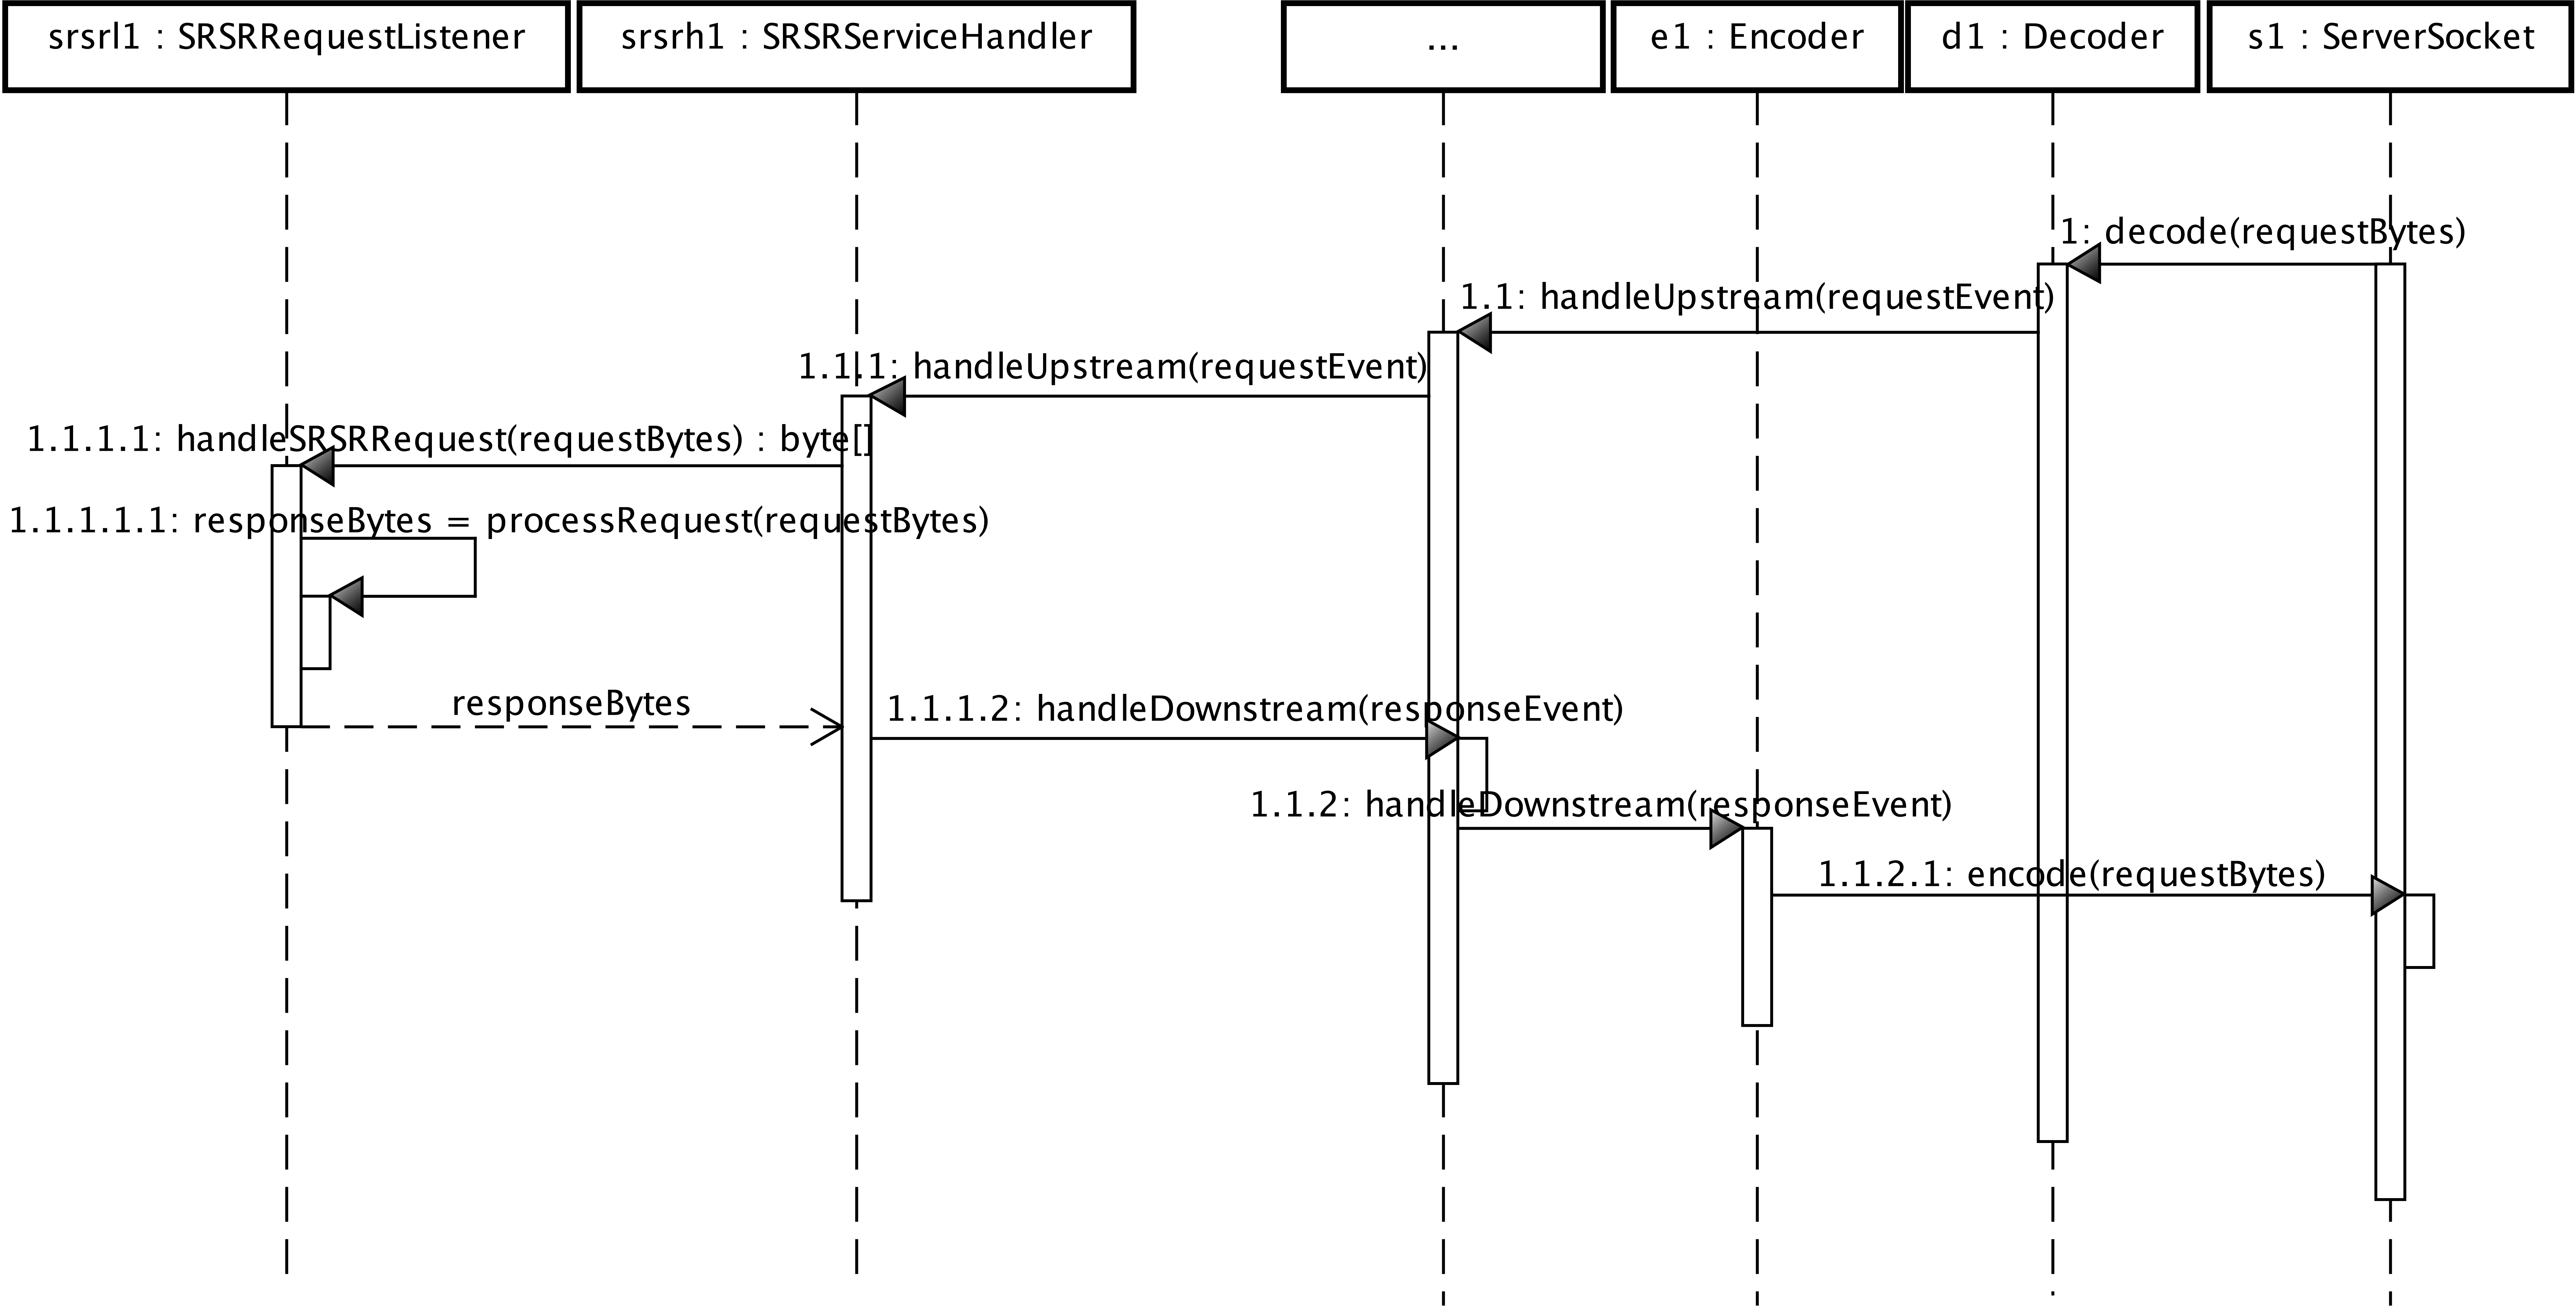
\includegraphics[width=12 cm]{img/sequence_srsr.png}
%\label{fig:sequence_srsr}
%\caption{Ablauf eines SingleRequestSingleResponse-Response}
%\end{figure}

\myfig{sequence_srsr}{sequenz}

Der Ablauf ist dabei wie folgt: Der Server-Socket liest bytes und reicht diese an den entsprechenden (Protobuf)-Decoder weiter. Dieser dekodiert die Nachricht und erzeugt daraus eine Protokoll-Nachricht. Diese wird als ChannelEvent upstream "uber die registrierten ChannelHandler an den SingleRequestSingleResponseServiceHandler weitergereicht. Der verantwortliche registrierte SingleRequestSingleResponseRequestListener bekommt den Payload "ubergeben, arbeitet den Request-Payload ab und gibt einen Response-Payload zur"uck an den SingleRequestSingleResponseRequestListener der daraus eine korrespondierende Response-Protokoll-Nachricht erzeugt. Diese Nachricht wird dann "uber die Handler der Pipeline downstream zum (Protobuf-)Dekoder durchgereicht. Der Dekoder serialisiert die bytes und sendet diese an den Client-Socket zur"uck.

Der Ablauf f"ur die weiteren Nachrichtentypen des Message Exchange Pattern ist dabei analog, wobei sich jeweils nur der ServiceHandler und RequestListener ver"andert.

\subsubsection{RequestResponseChannel}
Wie bereits in der ChannelArchitektur im Abschnitt \ref{subsec:mep-arch-channel} des Entwurfskapitel beschrieben, besitzt Ubermep neben dem UnicastMulticastChannel eigene RequestResponseChannel, namentlich {\it SingleRequestSingleResponseChannel} bzw. {\it MultiResponseChannel}. Im Folgenden werden nun diese beiden Channels n"aher beschrieben. Das Zusammenspiel der verschiedenen Channels ist dabei in Abbildung \ref{fig:mep-app_srsr_mr_channel} veranschaulicht.

\paragraph{SingleRequestSingleResponseChannel} 
"Uber den SingleRequestSingleResponseChannel k"onnen ausschlie"slich SingleRequestSingleResponseRequests versendet werden. Dabei ist einzig die folgende Methode von Bedeutung:

\myfig[110mm]{mep-app_srsr_mr_channel}{Handling der RequestResponse-Events in Ubermep}

\begin{itemize}
\item {\it write(SingleRequestSingleResponseRequest request)} sendet einen SingleRequestSingleResponseRequest "uber den SingleRequestSingleResponseChannel. Der Response wird als Future-Objekt zur"uckgegeben. Eine genaue Beschreibung der zur"uckgelieferten Response findet sich weiter unten im Abschnitt \ref{subsec:ubermep_core_msg}.
\end{itemize}

\paragraph{MultiResponseChannel}"Uber den MultiResponseChannel k"onnen ausschlie"slich MultiResponseRequests, namentlich SingleRequestMultiResponseRequest bzw. MultiRequestMultiResponseRequest versendet werden. Dabei ist einzig die folgenden Methode von Bedeutung:

\begin{itemize}
\item {\it write(Request request)} sendet einen MultiResponseRequest "uber den MultiResponseChannel. Der Response wird als Future-Objekt zur"uckgegeben. Eine genaue Beschreibung der zur"uckgelieferten Response findet sich weiter unten im Abschnitt \ref{subsec:ubermep_core_msg}.
\end{itemize}

\subsubsection{UbermepRpcChannel}
Ubermep besitzt einen eigenen Channel f"ur den Aufruf von Remote Procedure Calls, den UbermepRpcChannel. Mittels diesem Channel k"onnen Stubs generiert werden, "uber die dann der RPC aufgerufen werden kann. Die, f"ur den Aufruf entscheidenen Methoden, bezieht der UbermepRpcChannel aus dem Protobuf-Projekt. Die Abbildung \ref{fig:Dependencies_UbermepRpcChannel} veranschaulicht hierbei die Abh"angigkeiten. Die Methoden haben dabei die folgende Bedeutung:

\begin{itemize}
\item {\it callBlockingMethod(Descriptors.MethodDescriptor method, ...)} ruft einen blockierenden Remote Procedure Call auf und gibt die Antwort als Protokoll-Nachricht zur"uck. Blockierend hierbei bedeutet, das diese Methode solange den Aufrufer \emph{blockiert} bis eine Antwort empfangen wurde.
\item {\it callMethod(Descriptors.MethodDescriptor method, ...)} ruft einen nicht-blockierende Remote Procedure Call auf und gibt die Antwort als Protokoll-Nachricht in dem als Parameter "ubergebenen Callback zur"uck, wobei der Aufrufer hierbei \emph{nicht blockiert} wird.
\end{itemize}

\myfig{Dependencies_UbermepRpcChannel}{Abh"angigkeiten des UbermepRpcChannel}

\subsection{Messaging}
\label{subsec:ubermep_core_msg}
Im Folgenden Abschnitt werden nun die von Ubermep unterst"utzten Nachrichten-Pattern spezifiziert. Zuerst werden die Nachrichten des UnreliableMessaging-Pattern beschrieben danach die Nachrichten des ReliableMessaging.

In der nun folgenden Spezifikation haben dabei die verwendeten Eigenschaften die folgende Bedeutung:

\begin{itemize}
\item {\bf Parameter}: die der Nachricht zu "ubergebenen Parameter
\item {\bf PayloadListener}: der verantwortliche PayloadListener server-seitig zum Lesen des Request-Inhalts und Schreiben des Response-Inhalts
\item {\bf Response}: die zu erwartende Response bei erfolgreichem ausliefern der Nachricht
\item {\bf Optionale Parameter}: die der Nachricht optional zu "ubergebenen Parameter, wobei diese immer "uber entsprechende {\it Setter} gesetzt werden
\item {\bf Erfolgreich ausgeliefert bei}: gibt an, wann eine Nachricht als \emph{Erfolgreich ausgeliefert} gilt. Nur dann wird auch die entsprechende Response zur"uckgegeben
\item {\bf ProgressListener}: das zu implementierende Interface client-seitig
\item {\bf Zur"uckgeliefert bei}: gibt an, wann eine Nachricht an den Sender zur"uckgeliefert wird
\end{itemize}

\subsubsection{UnreliableRequest}
In diesem Abschnitt werden nun die Nachrichten des UnreliableMessaging-Pattern beschrieben.

\paragraph{UnreliableUnicastRequest}
Ein UnreliableUnicastRequest ist wie folgt spezifiziert:

%\begin{table}[h]
 %\caption{UnreliableUnicastRequest}
\begin{tabular}{|l|l|}
\hline 
{\bf Parameter} & remoteAddress : UPAddress \\
& payload : byte[] \\
\hline 
{\bf PayloadListener} & UnicastMulticastRequestListener (lesen) \\
\hline
{\bf Response} & keine \\
\hline
\end{tabular}
%\end{table}

\paragraph{UnreliableMulticastRequest}
Ein UnreliableMulticastRequest ist wie folgt spezifiziert:

%\begin{table}[h]
% \caption{UnreliableMulticastRequest}
\begin{tabular}{|l|l|}
\hline 
{\bf Parameter} & remoteAddresses : Collection$<$UPAddress$>$ \\
& payload : byte[] \\
\hline 
{\bf PayloadListener} & UnicastMulticastRequestListener (lesen) \\
\hline
{\bf Response} & keine \\
\hline
\end{tabular}
%\end{table}

\subsubsection{ReliableRequest}
In diesem Abschnitt werden die Nachrichten des ReliableMessaging-Pattern spezifiziert.

\paragraph{ReliableUnicastRequest}
Ein ReliableUnicastRequest ist wie folgt spezifiziert:

%\begin{table}[h]
% \caption{ReliableUnicastRequest}
\begin{tabular}{|l|l|}
\hline 
{\bf Parameter} & remoteAddress : UPAddress \\
& payload : byte[] \\
\hline
 {\bf optionale Parameter} & timeOut : int \\
 & timeOutUnit : TimeUnit \\
 \hline
 {\bf PayloadListener} & UnicastMulticastRequestListener (lesen) \\
 \hline
 {\bf Response} & ReliableUnicastResponse \\
 \hline
  {\bf Erfolgreich ausgeliefert bei} & Eingang der Nachricht am Empf"anger-Peer \\
  \hline
\end{tabular}
%\end{table}

\paragraph{ReliableMulticastRequest}
Ein ReliableMulticastRequest ist wie folgt spezifiziert:

%\begin{table}[h]
% \caption{ReliableMulticastRequest}
\begin{tabular}{|l|l|}
\hline 
{\bf Parameter} & remoteAddresses : Collection$<$UPAddress$>$ \\
& payload : byte[] \\
\hline
 {\bf optionale Parameter} & timeOut : int \\
 & timeOutUnit : TimeUnit \\
 \hline
 {\bf PayloadListener} & UnicastMulticastRequestListener (lesen) \\
 \hline
 {\bf Response} & ReliableMulticastResponse \\
 \hline
  {\bf Erfolgreich ausgeliefert bei} & Eingang der Nachricht am Empf"anger-Peer \\
  \hline
\end{tabular}
%\end{table}

Anmerkung: Eine ReliableMulticastResponse enth"alt die Responses als Map. Die Responses werden dabei in der Map-"ublichen Weise,  also als \emph{Key,Value}-Paar   
der Response-Map hinzugef"ugt. Der {\it Key} entspricht dabei der UPAddress des geantworteten Peers, der {\it Value} einer einzelnen Response vom Typ  {\it ReliableMulticastResponse.SingleReliableMulticastResponse}.

\paragraph{SingleRequestSingleResponseRequest}
Ein SingleRequestSingleResponseRequest ist wie folgt spezifiziert:

%\begin{table}[h]
% \caption{SingleRequestSingleResponseRequest}
\begin{tabular}{|l|l|}
\hline 
{\bf Parameter} & remoteAddress : UPAddress \\
& payload : byte[] \\
\hline
 {\bf optionale Parameter} & timeOut : int \\
 & timeOutUnit : TimeUnit \\
 \hline
 {\bf PayloadListener} & SingleRequestSingleResponseRequestListener\\
 & (lesen und schreiben) \\
 \hline
 {\bf Response} & SingleRequestSingleResponseResponse \\
 \hline
  {\bf Erfolgreich ausgeliefert bei} & Eingang der Nachricht am Empf"anger-Peer {\bf und} \\
 & erfolgreicher Verarbeitung eines PayloadListener \\
  \hline
\end{tabular}
%\end{table}

\paragraph{SingleRequestMultiResponseRequest}
Ein SingleRequestMultiResponseRequest ist wie folgt spezifiziert:

%\begin{table}[h]
% \caption{SingleRequestMultiResponseRequest}
\begin{tabular}{|l|l|}
\hline 
{\bf Parameter} & remoteAddress : UPAddress \\
& payload : byte[] \\
\hline
 {\bf optionale Parameter} & timeOut : int \\
 & timeOutUnit : TimeUnit \\
 \hline
 {\bf PayloadListener} & MultiResponseRequestListener\\
 & (lesen und schreiben) \\
 \hline
  {\bf ProgressListener} & ProgressListenerRunnable \\
 \hline
 {\bf Response} & SingleRequestMultiResponseResponse \\
 \hline
  {\bf Erfolgreich ausgeliefert bei} & Eingang der Nachricht am Empf"anger-Peer {\bf und} \\
 & erfolgreicher Verarbeitung eines PayloadListener \\
  \hline
\end{tabular}
%\end{table}

%Anmerkung: Eine SingleRequestMultiResponse-Response enth"alt die Responses als Map. Die Responses werden dabei in der Map-"ublichen Weise,  also als \emph{Key,Value}-Paar   
%der Response-Map hinzugef"ugt. Der {\it Key} entspricht dabei der UPAddress des geantworteten Peers, der {\it Value} einer einzelnen Response vom Typ  {\it SingleMultiResponseResponse}.

\paragraph{MultiRequestMultiResponseRequest}
Ein MultiRequestMultiResponseRequest ist wie folgt spezifiziert:

%\begin{table}[h]
% \caption{MultiRequestMultiResponseRequest}
\begin{tabular}{|l|l|}
\hline 
{\bf Parameter} & remoteAddresses : Collection$<$UPAddress$>$ \\
& payload : byte[] \\
\hline
 {\bf optionale Parameter} & timeOut : int \\
 & timeOutUnit : TimeUnit \\
 \hline
 {\bf PayloadListener} & MultiResponseRequestListener\\
 & (lesen und schreiben) \\
 \hline
  {\bf ProgressListener} & ProgressListenerRunnable \\
 \hline
 {\bf Response} & MultiRequestMultiResponseResponse \\
 \hline
  {\bf Erfolgreich ausgeliefert bei} & Eingang der Nachricht am Empf"anger-Peer {\bf und} \\
 & erfolgreicher Verarbeitung eines PayloadListener \\
  \hline
\end{tabular}
%\end{table}

Anmerkung: Eine MultiResponse-Response enth"alt die Responses als Map. Die Responses werden dabei in der Map-"ublichen Weise,  also als \emph{Key,Value}-Paar   
der Response-Map hinzugef"ugt. Der {\it Key} entspricht dabei der UPAddress des geantworteten Peers, der {\it Value} einer einzelnen Response vom Typ  {\it SingleMultiResponseResponse}.

\subsubsection{ReliableResponse}
Einzig Nachrichten des oben beschriebenen ReliableMessaging-Pattern liefern Responses zur"uck. Dabei gibt es, wie oben spezifiziert, f"ur einen erfolgreich ausgelieferten ReliableRequest einen korrespondierenden ReliableResponse. Des weiteren gibt es f"ur diesen Request ReliableResponses bei nicht erfolgreicher "Ubertragung. Im Folgenden werden nun diese beschrieben.

\paragraph{ErrorResponse}
Eine ErrorResponse ist wie folgt spezifiziert:

%\begin{table}[h]
% \caption{MultiRequestMultiResponseRequest}
\begin{tabular}{|l|l|}
\hline 
{\bf Parameter} & request : Request \\
& localAddress : UPAddress \\
& cause : Throwable \\
 \hline
  {\bf Zur"uckgeliefert bei} & Fehlerhafter "Ubertragung einer Nachricht \\
  \hline
\end{tabular}
%\end{table}

\paragraph{TimeOutResponse}
Eine TimeOutResponse ist wie folgt spezifiziert:

%\begin{table}[h]
% \caption{MultiRequestMultiResponseRequest}
\begin{tabular}{|l|l|}
\hline 
{\bf Parameter} & request : Request \\
& localAddress : UPAddress \\
 \hline
  {\bf Zur"uckgeliefert bei} & TimeOut w"ahrend der Auslieferung, ausgel"ost durch: \\
  & TimeOut des Request wenn gesetzt, \\
  & sonst DefaultTimeOut (siehe dazu Abschnitt \ref{subsec:ubermep-core_konfiguration} ) \\
  \hline
\end{tabular}
%\end{table}

\subsection{Konfiguration}
\label{subsec:ubermep-core_konfiguration}
Die Konfiguration von Ubermep erfolgt "uber das konfigurieren der einzelnen Peers des Netzwerks. Dies geschieht "uber Variablen der Klasse {\it PeerConfig}. Die nun folgenden Spezifikationen sind dabei wie folgt aufgebaut:

\paragraph{\{Variablenname\}}
\begin{itemize}
\item {\bf \{Verwendung\}}
\item {\bf \{Typ\}}
\item  {\bf \{DefaultValue\}}
\end{itemize}

\subsubsection{Konfiguration eines Peers}
Die Konfiguration eines Peers ist wie folgt spezifiziert: 

\paragraph{CORE\_POOL\_SIZE}
\begin{itemize}
\item {\bf Verwendung}: Die Gr"o"se der von Uberlay verwendeten ThreadPools 
\item {\bf Typ}: int
\item  {\bf DefaultValue}: 10
\end{itemize}
	
\paragraph{DEFAULT\_TIMEOUT}
\begin{itemize}
\item {\bf Verwendung}: Die DefaultTimeOut f"ur ReliableRequests.
\item {\bf Typ}: int
\item  {\bf DefaultValue}: 30
\end{itemize}

\paragraph{DEFAULT\_TIMEOUT\_TIMEUNIT}
\begin{itemize}
\item {\bf Verwendung}: Die Default-Zeiteinheit der DEFAULT\_TIMEOUT
\item {\bf Typ}: TimeUnit
\item  {\bf DefaultValue}: TimeUnit.SECONDS
\end{itemize}

\paragraph{UberlayModule.RTT\_REQUEST\_INTERVAL}
\begin{itemize}
\item {\bf Verwendung}: Das Interval in dem die RoutingTabellen eines Peers mittels des RoundTripTime-Protokolls von Uberlay aktualisiert werden. (siehe dazu Abschnitt \ref{subsec:uberlay-rtt} im Grundlagenkapitel)
\item {\bf Typ}: int
\item  {\bf DefaultValue}: 10
\end{itemize}

\paragraph{UberlayModule.RTT\_REQUEST\_INTERVAL\_TIMEUNIT}
\begin{itemize}
\item {\bf Verwendung}: Die Default-Zeiteinheit des RTT\_REQUEST\_INTERVAL
\item {\bf Typ}: int
\item  {\bf DefaultValue}: TimeUnit.SECONDS
\end{itemize}

\section{Beispiele}
\label{sec:beispiele}
Im Folgenden soll nun anhand von Beispielen die Funktionalit"at von Ubermep veranschaulicht werden. Dazu wird ein kleines Peer-to-Peer Netzwerk mit 3 Knoten erzeugt, "uber die dann Nachrichten des Message Exchange Pattern versendet werden k"onnen.

\subsection{Aufbau eines Peer-to-Peer Netzwerk}
Im nun folgenden Beispiel wird ein Peer-to-Peer Netzwerk wie folgt aufgebaut:

\myfig{example_p2p_network}{Aufbau eines einfachen Peer-to-Peer Netzwerk}

Der entsprechende Quellcode sieht dabei wie folgt aus:

\lstset{caption=Aufbau eines einfachen Peer-to-Peer Netzwerk,tabsize=4,language=Java,firstnumber=1, label=bsp:createPeer}
\begin{lstlisting}
// Peers erzeugen ... 
Peer server = new PeerImpl(new UPAddress("urn:itm:1"), 
	new InetSocketAddress("0.0.0.0", 8080));
Peer transitHost = new PeerImpl(new UPAddress("urn:itm:2"), 
	new InetSocketAddress("0.0.0.0", 8081), 
	new InetSocketAddress("0.0.0.0", 8080));
Peer client = new PeerImpl(new UPAddress("urn:itm:3"), 
	new InetSocketAddress("0.0.0.0", 8082), 
	new InetSocketAddress("0.0.0.0", 8081));

// Peers starten ...
server.start();
transitHost.start();
client.start();

// ... kommuniziere ein wenig ...

// Peers stoppen
client.stop();
transitHost.stop();
server.stop();
\end{lstlisting}

\subsection{Kommunikation}

\nomenclature{WSN}{Wireless Sensor Network}

Nachdem nun das Netzwerk aufbaut ist, kann "uber die Knoten kommuniziert werden. In den nun folgenden Beispielen sollen Nachrichten erzeugt und versendet werden, um ausgew"ahlte Peers (Nodes) zu \emph{flashen}. \emph{Flashen} bedeutet hier: Das Aufspielen einer neuen Firmware auf einem Knoten. Diese Funktionalit"at spielt z.B. eine Rolle in {\it Wireless Sensor Networks (WSN's)}. Daf"ur werden in den folgenden Beispielen der String {\tt flashNode} als ByteArray "ubertragen und ausgewertet.

\subsubsection{Unreliable Messaging}
Um nun Unicast- bzw. Multicast-Requests f"ur das flashen von Nodes verarbeiten zu k"onnen, muss zuerst der entsprechende UnicastMulticastRequestListener wie folgt erzeugt werden, dabei sei angenommen das eine entsprechende Methode {\it flashNode()} mit der oben beschriebenen Funktionalit"at vorhanden ist:

\lstset{caption=Erzeugen eines UnicastMulticastRequestListener,tabsize=2,language=Java,firstnumber=1, label=bsp:createRequestListener}
\begin{lstlisting}
UnicastMulticastRequestListener flashNodeUnicastMulticastRequestListener = new UnicastMulticastRequestListener() {
	public boolean handleUnicastMulticastRequest(String senderUrn, byte[] payload) {
		if (new String(payload).equals("flashNode")) {
			// aufrufen von flashNode()
			flashNode();
			return true;
		} else {
			return false;
		}
	}
};
\end{lstlisting}

Nun muss noch der {\it flashNodeUnicastMulticastRequestListener} am entsprechenden Peer server-seitig hinzugef"ugt werden.

\lstset{caption=Hinzuf"ugen eines UnicastMulticastRequestListener,tabsize=2,language=Java,firstnumber=1, label=bsp:addUnicastMulticastRequestListener}
\begin{lstlisting}
server.addRequestListener(flashNodeUnicastMulticastRequestListener);
\end{lstlisting}

\paragraph{UnreliableUnicastRequest}
Anschlie"send kann ein entsprechender UnreliableUnicastRequest an den Server wie folgt versendet werden:

\lstset{caption=Senden eines UnreliableUnicastRequest,tabsize=2,language=Java,firstnumber=1, label=bsp:sendUnrelUnicast}
\begin{lstlisting}
UnreliableRequest request = new UnreliableUnicastRequest(server.getLocalUPAddress(), "flashNode".getBytes());
client.send(request);
\end{lstlisting}

\paragraph{UnreliableMulticastRequest} 
Der Aufruf eines UnreliableMulticastRequest geschieht analog zu dem eines UnreliableUnicastRequest.
\lstset{caption=Senden eines UnreliableMulticastRequest,tabsize=2,language=Java,firstnumber=1, label=bsp:sendUnrelMulticast}
\begin{lstlisting}
List<UPAddress> urns = new ArrayList<UPAddress>() {{
	add(server.getLocalUPAddress());
	add(...);
}};

UnreliableRequest request = new UnreliableMulticastRequest(urns, "flashNode".getBytes());
client.send(request);
\end{lstlisting}

\subsubsection{Reliable Messaging}
Nachrichten des Reliable Messaging Patterns k"onnen als blockierende als auch als nicht-blockierende Aufrufe versendet werden. Im Folgenden Beispiel werden nun die beiden Aufrufe dargestellt:

\lstset{caption=Blockierender und nicht-blockierender Nachrichtenempfang,tabsize=2,language=Java,firstnumber=1, label=bsp:blockingNonBlockingResponse}
\begin{lstlisting}
final ListenableFuture<Response> responseFuture = client.send(request);

//blockierender Aufruf
Response response = responseFuture.get();

//nicht-blockierender Aufruf
responseFuture.addListener(new Runnable() {
	public void run() {
		Response response = responseFuture.get();
	}}, new ScheduledThreadPoolExecutor(1));
...
\end{lstlisting}

In den folgenden Beispielen werden zur Vereinfachung nur blockierende Aufrufe beschrieben.

\paragraph{ReliableUnicastRequest} 
Mit Hilfe eines ReliableUnicastRequest kann nun "uberpr"uft werden, ob die Methode {\it flashNode()} tats"achlich aufgerufen wurde.
\lstset{caption=Senden eines ReliableUnicastRequest als blockierender Aufruf,tabsize=2,language=Java,firstnumber=1, label=bsp:sendRelUnicast}
\begin{lstlisting}
ReliableRequest request = new ReliableUnicastRequest(server.getLocalUPAddress(), "flashNode".getBytes());
Future<Response> responseFuture = client.send(request);

Response response = responseFuture.get();
if (response instanceof ReliableUnicastResponse){
	// tu was mit Response
}
\end{lstlisting}

\paragraph{ReliableMulticastRequest}
Der Aufruf eines ReliableMulticastRequest geschieht analog zu dem eines ReliableUnicastRequest.
\lstset{caption=Senden eines ReliableMulticastRequest,tabsize=2,language=Java,firstnumber=1,literate={�}{{\"u}}1, label=bsp:sendRelMulticast}
\begin{lstlisting}
List<UPAddress> urns = new ArrayList<UPAddress>() {{
	add(transitHost.getLocalUPAddress());
	add(...);
}};

ReliableRequest request = new ReliableMulticastRequest(urns, "flashNode".getBytes());
Future<Response> responseFuture = client.send(request);

Response response = responseFuture.get();
// "uberpr�fe Responses ... �ber: response.getResponses()
\end{lstlisting}

\paragraph{SingleRequestSingleResponseRequest}
Um einen SingleRequest\-Single\-Response\-Request f"ur das flashen eines Nodes verarbeiten zu k"onnen, muss zuerst der entsprechende SingleRequestSingleResponseRequestListener server-seitig wie folgt erzeugt und hinzugef"ugt werden, dabei sei auch hier angenommen das eine entsprechende Methode {\it flash\-Node()} mit der beschriebenen Funktionalit"at vorhanden ist:
\lstset{caption=Erstellen eines SingleRequestSingleResponseRequestListener,tabsize=2,language=Java,firstnumber=1, label=bsp:createSRSRRequestListener}
\begin{lstlisting}
SingleRequestSingleResponseRequestListener flashNodeSingleRequestSingleResponseRequestListener = new SingleRequestSingleResponseRequestListener() {
	public byte[] handleSingleRequestSingleResponseRequest(String senderUrn, byte[] payload) throws UbermepExceptionEvent {
		if (new String(payload).equals("flashNode")) {
			try {
				// aufrufen von flashNode()
				flashNode();
				return "flashNode: Done".getBytes();
			} catch (Exception e){
				throw 
					new UbermepSingleResponseExceptionEvent(e.getCause());
			}
		} else {
			return null;
		}
	}
};

server.addRequestListener(flashNodeSingleRequestSingleResponseRequestListener);
\end{lstlisting}

Anschlie"send kann nun mit Hilfe eines SingleRequestSingleResponseRequest "uberpr"uft werden, ob die Methode {\it flashNode()} tats"achlich aufgerufen wurde:
\lstset{caption=Senden eines SingleRequestSingleResponseRequest,tabsize=2,language=Java,firstnumber=1,literate={�}{{\"u}}1, label=bsp:sendSRSR}
\begin{lstlisting}
ReliableRequest request = new SingleRequestSingleResponseRequest(server.getLocalUPAddress(), "flashNode".getBytes());
Future<Response> responseFuture = client.send(request);

Response response = responseFuture.get();
if (response instanceof SingleRequestSingleResponseResponse){
	// tu was mit Response, z.B. payload �berpr�fen
}
\end{lstlisting}

\paragraph{SingleRequestMultiResponseRequest}
Um einen Multi\-Response\-Request f"ur das flashen eines Nodes verarbeiten zu k"onnen, muss zuerst der entsprechende MultiResponseRequestListener server-seitig wie folgt erzeugt und hinzugef"ugt werden, dabei sei auch hier angenommen das eine Methode {\it flash\-Node()} mit der bereits beschriebenen Funktionalit"at vorhanden ist ,wobei die Methode hier den Fortschritt in Prozent als Integer-Wert zur"uckgibt:

\lstset{caption=Hinzuf"ugen eines MultiResponseRequestListener,tabsize=2,language=Java,firstnumber=1, label=bsp:createMRRequestListener}
\begin{lstlisting}
MultiResponseRequestListener flashNodeMultiResponseRequestListener = new MultiResponseRequestListener() {
	public boolean handleMultiResponseRequest(MultiResponseHandle responseHandle, String senderUrn, byte[] payload) throws UbermepExceptionEvent {
		if (new String(payload).equals("flashNode")) {
			// aufrufen von flashNode()
			int percentDone = flashNode();
			while(percentDone < 50){;}
			// wenn flashNode() zu 50% fertig
			responseHandle.handleSingleResponse("flashNode:50% done".getBytes(), 1, 2);
			while(percentDone < 100){;}
			// wenn flashNode() fertig
			responseHandle.handleSingleResponse("flashNode:100% done".getBytes(), 2, 2);
			return true;
		} else {
			return false;
		}
	}
};

server.addRequestListener(flashNodeMultiResponseRequestListener);
\end{lstlisting}

Anschlie"send kann nun mit Hilfe eines SingleRequestMultiResponseRequest "uberpr"uft werden, ob die Methode {\it flashNode()} tats"achlich aufgerufen wurde und wie der Fortschritt ist.
\lstset{caption=Senden eines SingleRequestMultiResponseRequest,tabsize=2,language=Java,firstnumber=1, label=bsp:sendSRMR}
\begin{lstlisting}
ReliableRequest request = new SingleRequestMultiResponseRequest(server.getLocalUPAddress(), "flashNode".getBytes());
Future<Response> responseFuture = client.send(request);

Response response = responseFuture.get();
if (response instanceof SingleRequestMultiResponseResponse){
	// �berpr�fe Responses ... �ber: response.getResponses()
}
\end{lstlisting}

\paragraph{MultiRequestMultiResponseRequest}
Der Aufruf eines MultiRequestMultiResponseRequest geschieht analog zu dem eines SingleRequestMultiResponseRequest.
\lstset{caption=Senden eines MultiRequestMultiResponseRequest,tabsize=2,language=Java,firstnumber=1, label=bsp:sendMRMR}
\begin{lstlisting}
List<UPAddress> urns = new ArrayList<UPAddress>() {{
	add(server.getLocalUPAddress());
	add(...);
}};

ReliableRequest request = new MultiRequestMultiResponseRequest(urns, "flashNode".getBytes());
Future<Response> responseFuture = client.send(request);

//auf Response warten
Response response = responseFuture.get();
if (response instanceof MultiRequestMultiResponseResponse){
	// "uberpr�fe Responses ... �ber: response.getResponses()
}
\end{lstlisting}

Ein ProgressListener f"ur MultiResponse-Nachrichten l"a"st sich wie folgt client-seitig hinzuf"ugen:

\lstset{caption=Verwenden eines ProgressListener,tabsize=2,language=Java,firstnumber=1, label=bsp:createProgressListener}
\begin{lstlisting}
//erzeuge ProgressListenerRunnable
ProgressListenerRunnable progressListenerRunnable = new ProgressListenerRunnable() {
	public void progress(String senderUrn, byte[] payload, int current, int total) {
		//tu etwas mit einzeln empfangener Response z.B. 
		log.info("received: " + current + " of " + total);
	}

	public void run() {
		//tu etwas mit komplett empfangener MultiResponse z.B. 
		Response response = responseFuture.get();
	}
};

// ProgressListener dem ResponseFuture hinzuf�gen
responseFuture.addListener(progressListenerRunnable, new ScheduledThreadPoolExecutor(2));
\end{lstlisting}


\subsubsection{RPC}
In dem nun folgenden Beispiel soll veranschaulicht werden, wie Remote Procedure Calls in Ubermep aufgerufen werden k"onnen. Dies wird mittels der bereits beschriebenen  Funktionalit"at des flashens von Nodes veranschaulicht. Dazu mu"s zuerst mittels der Protobuf-IDL (siehe Abschnitt \ref{sec:google-protobuf} im Grundlagenkapitel) ein FlashNodeServiceProtokoll erzeugt werden. Im Listing \ref{lst:ubermep_flash_node_rpc} ist daf"ur ein Beispiel-Protokoll erstellt worden, welches anschlie"send mittels des protoc-Compiler in ein Java-Klasse "ubersetzt wird. Der Aufruf erfolgt dabei "uber einen FlashNodeRequest, welcher den Parameter {\it delay} enth"alt. Das Ergebnis wird "uber den FlashNodeResponse zur"uckgegeben, wobei daf"ur der Parameter {\it success} hinzugef"ugt wurde.
\lstinputlisting[language=Python,label=lst:ubermep_flash_node_rpc,caption=FlashNodeServiceProtocol.proto]{lst/FlashNodeServiceProtocol.proto}

Anschlie"send wird eine Implementierung des Service-Interface erzeugt, wobei im Folgenden Beispiel eine Implementierung des BlockingInterface verwendet wurde. 
Im Folgenden sei auch hier angenommen das eine Methode {\it flash\-Node()} mit der bereits beschriebenen Funktionalit"at vorhanden ist ,wobei die Methode hier als Parameter einen {\it delay} als Verz"ogerung des Aufrufs "ubergeben bekommt.

\lstset{caption=Implementierung des FlashNodeBlockingService,tabsize=2,language=Java,firstnumber=1, label=bsp:createBlockingService}
\begin{lstlisting}
public class FlashNodeBlockingServiceImpl implements FlashNodeServiceProtocol.FlashNodeService.BlockingInterface, RpcBlockingService{
	@Override
	public FlashNodeServiceProtocol.FlashNodeResponse flashNode(RpcController controller, FlashNodeServiceProtocol.FlashNodeRequest request) throws ServiceException {
		// aufrufen von flashNode(delay)
		flashNode(request.getDelay());
		return FlashNodeServiceProtocol.FlashNodeResponse.newBuilder().setSuccess(true).build();
	}

	@Override
	public BlockingService getRpcBlockingService() {
		return FlashNodeServiceProtocol.FlashNodeService.newReflectiveBlockingService(this);
	}
}
\end{lstlisting}
Im Folgenden soll nun ein RPC, "uber dem bereits oben erzeugten Peer-to-Peer Netzwerk, vom Client auf dem Server ausgef"uhrt werden. Hierf"ur muss zuerst die {\it FlashNodeBlockingServiceImpl} am entsprechenden Peer server-seitig hinzugef"ugt werden. Anschlie"send kann ein entsprechender FlashNodeRequest mittlels des RPC-Channel auf dem Server wie folgt aufgerufen werden:
\lstset{caption=Aufruf des FlashNodeBlockingService,tabsize=2,language=Java,firstnumber=1,literate={�}{{\"u}}1, label=bsp:callBlockingService}
\begin{lstlisting}
//Service am Server registrieren
server.registerService(new FlashNodeBlockingServiceImpl());

// erzeuge RPC-Request mit delay=10
FlashNodeServiceProtocol.FlashNodeRequest request = FlashNodeServiceProtocol.FlashNodeRequest.newBuilder().setDelay(10).build();

// hole RPC-Channel
UbermepRpcChannel blockingServerRpcChannel = client.getRpcChannel(blockingServerUrn);
// erzeuge neuen Blocking-Stub f�r FlashNodeService mittels RPC-Channel
FlashNodeServiceProtocol.FlashNodeService.BlockingInterface blockingService = FlashNodeServiceProtocol.FlashNodeService.newBlockingStub(blockingServerRpcChannel);

try {
	//rufe flashNodeService auf
	FlashNodeServiceProtocol.FlashNodeResponse rpcResponse = blockingService.flashNode(new RpcControllerImpl(), request);

	// tu was mit RPC-Response, z.B. success �berpr�fen	
} catch (ServiceException e) {
	// tu was mit ServiceException
}
\end{lstlisting}

Der Aufruf eines (non-blocking)-Service ist analog und soll deshalb hier nicht weiter vertieft werden. Nur soviel: der Service-Aufruf ben"otigt eine zus"atzliche (non-blocking)-Service-Implementierung sowie einen Callback der aber einfach "uber:
\lstset{caption=Erzeugung eines FlashNodeServiceCallback,tabsize=2,language=Java,firstnumber=1,literate={�}{{\"u}}1, label=bsp:createServiceCallback}
\begin{lstlisting}
MEPRpcCallback<FlashNodeServiceProtocol.FlashNodeResponse> callback = new RpcCallbackImpl<FlashNodeServiceProtocol.FlashNodeResponse>();
\end{lstlisting}
erzeugt werden kann.

\section{Zuk"unftige Erweiterungen}
\label{sec:zukunft}

Folgende Erweiterungen sind fest f"ur die n"ahere Zukunft eingeplant:
\todo{ausf"uhrlicher...}
\begin{itemize}
\item Bilden von Peer-to-Peer-Communities und in diesem Zusammenhang auch Erweiterung um {\it Broadcast}-Messaging f"ur einzelne Communities
\item Hinzuf"ugen einer Peer-to-Peer-Proxy-Funktionalit"at und daraus resultierend auch das Hinzuf"ugen einer Firewall-Funktionalit"at f"ur bestimmte Peers zum kontrollieren von deren Netzwerkverkehr
\item Erweiterung des RoundTripTime-Protokoll von Uberlay um Anpassbarkeit der Zeitintervalle, z.B. mittels dem {\it Trickle}-Algorithmus \cite{trickle}
\end{itemize} 
	\chapter{Evaluation}
\label{cha:evaluation}

\section{Netzwerk-Topologien}
In den Abbildungen \ref{fig:Evaluations_Szenario_SingleHop} und \ref{fig:Evaluations_Szenario_MultiHop} ist der Aufbau der Evaluationsszenarios zu sehen. Dabei handelt es sich zum Einem um Single-Hop- und zum Anderen um Multi-Hop- Netzwerke. Die Nachrichten zur Evaluation werden dabei immer von einem Peer A zu einem Peer B und ggf. zur"uckgesendet. Jeder Peer wird dabei als Loopback-Interface an einem Rechner gestartet. Damit die Evaluationsergebnisse mit Szenarien der realen Umwelt vergleichbar sind, wurde f"ur die Evaluation ein Emulator erzeugt, welcher eine "Ubertragungsrate von 16 MBit/s emuliert.
\myfig[7 cm]{Evaluations_Szenario_SingleHop}{Single-Hop-Topologie}
\myfig{Evaluations_Szenario_MultiHop}{Multi-Hop-Topologie}

\section{Evaluationskriterien}
Zur Evaluation der Implementierung wurden zwei Kriterien verwendet:
\begin{itemize}
\item "Ubertragungsdauer in Abh"angigkeit der Payload-Gr"o"se
\item "Ubertragungsdauer in Abh"angigkeit der Hop-Anzahl
\end{itemize}
Im Folgenden werden nun diese beiden Kriterien n"aher erl"autert.

\subsection{"Ubertragungsdauer in Abh"angigkeit der Payload-Gr"o"se}
Das Kriterium \emph{"Ubertragungsdauer in Abh"angigkeit der Payload-Gr"o"se} zeigt das Verh"altnis der "Uber\-tra\-gungs\-dauer zu der Gr"o"se des "ubertragenen Payloads. Dabei wurden Single Request Single Response-Nachrichten in einem Single-Hop-Netzwerk versendet. Die gemessene "Uber\-tra\-gungs\-dauer entspricht dabei der Zeit vom Versand einer Nachricht bis zum Empfang der Antwort. Dabei variiert die Gr"o"se des Request-Payloads, der Response-Payload aber ist immer jeweils 1 Byte gro"s. Mittels diesem Kriterium l"asst sich feststellen wie sich die "Uber\-tra\-gungs\-dauer, in Abh"angigkeit der Gr"o"se einer Nachricht, verh"alt.

\subsection{"Ubertragungsdauer in Abh"angigkeit der Hop-Anzahl}

Das Kriterium \emph{"Ubertragungsdauer in Abh"angigkeit der Hop-Anzahl} berechnet das Verh"altnis der "Uber\-tra\-gungs\-dauer zu der Anzahl an Hops in einem Netzwerk. Dabei wurde die "Uber\-tra\-gungs\-dauer f"ur ein SingleHop-Netzwerk, sowie MultiHop-Netzwerke der Gr"o"se 2, 3, 4 und 5 Hops gemessen. Des weiteren wurde die "Ubertragungszeit f"ur den Nachrichtenversand mittels Uberlay, sowie f"ur den Nachrichtenversand mittels Unicast, SingleRequestSingleResponse und RPC gemessen. Daf"ur wurden Nachrichten mit einer Gr"o"se $<$ 1 Byte "uber das entsprechende Netzwerk gesendet. Die gemessene "Uber\-tra\-gungs\-dauer f"ur Uberlay und Unicast entspricht dabei der Zeit vom Versand bis zum Empfang der Nachricht. F"ur SingleRequestSingleResponse und RPC entspricht die gemessene "Uber\-tra\-gungs\-dauer der Zeit vom Versand bis zum Empfang der Antwort, wobei f"ur RPC ein BlockingService verwendet wurde. Mittels diesem Kriterium l"asst sich feststellen inwieweit sich gegebenfalls die "Uber\-tra\-gungs\-dauer eines Nachrichtentyps zu der Anzahl an Hops verh"alt.  

Bei beiden Kriterien wurde die "Ubertragungszeit in bereits verbundenen Netzwerken gemessen, d.h. die ben"otigte Zeit zum Aufbau eines Netzwerks ist hier nicht inkludiert. 

\section{Testergebnisse}
F"ur das Generieren der Testl"aufe wurden Testprogramme mit Java geschrieben, welche die oben beschriebenen Netzwerk-Topologien erzeugen und "uber diesen die Nachrichten versendet, sowie die "Uber\-tra\-gungs\-dauer misst. Diese Ergebnisse werden in sogenannten \emph{Boxplots} dargestellt. Im Folgenden werden nun Boxplots erl"autert.

\subsection{Boxplot}
Ein Boxplot ist ein Diagramm, das zur grafischen Darstellung der Verteilung von Daten verwendet werden kann. Der Boxplot vermittelt dabei schnell einen "Uberblick, in welchem Bereich die Daten liegen und wie sie sich in diesem verteilen. Ein Beispiel-Boxplot ist dabei in Abbildung \ref{fig:evaluation_example} zu erkennen. Die Verteilung wird dabei mittels eines Medians, zwei Quartilen und den beiden Whiskern dargestellt. Im Folgenden werden nun Quartile, Whisker und der Median erkl"art.
\myfig{evaluation_example}{Boxplot-Beispiel}

\nomenclature{IQR}{Interquartilsabstand}

\paragraph{Quartil}
Das Quartil, begrenzt durch das \emph{Obere Quartil} und \emph{Untere Quartil}, beschreibt die mittleren 50 \% der Werte. Die L"ange vom oberen Quartil zum unteren Quartil entspricht dabei dem Interquartilsabstand (IQR), welcher die Streuung der Werte zeigt.
\paragraph{Whisker}
Der Whisker, begrenzt durch den \emph{Oberen Whisker} und \emph{Unteren Whisker}, beschreibt den gesamten Wertebereich, sofern die Werte dabei nicht au"serhalb des 1,5 -fachen IQR zum jeweiligen Quartil liegen. Sofern ein Wert ausserhalb des 1,5-fachen IQR liegt, wird dieser als \emph{Ausrei"ser} deklariert.
\paragraph{Median}
Ein Median ist der \emph{Zentralwert}, welcher die Mitte eines Wertebereichs zeigt. Daf"ur wird der Wertebereich der Gr"o"se nach geordnet. Der Wert in der Mitte entspricht dann dem Median. Ist die Anzahl der Werte gerade, wird das arithmetische Mittel der beiden mittleren Werte berechnet. Aus diesem Grund hat der Median die Eigenschaft, dass die eine H"alfte der Werte "uber diesem und die andere darunter liegt.

Die nun im Folgenden dargestellten Ergebnisse entsprechen einer Messung von 1.00 versendeten Nachrichten. Zu Testzwecken wurden auch bis zu 1000 Nachrichten versendet und deren "Ubertragungszeit gemessen. Dabei sind die entscheidenden Ergebnisse, wie Quartile, Whisker und Medians nahezu identisch, einige Ausrei"ser allerdings sorgten f"ur eine un"ubersichtliche Darstellung, weshalb die Messung auf 100 Nachrichten beschr"ankt wurde.

\subsection{"Ubertragungsdauer in Abh"angigkeit der Payload-Gr"o"se}

\myfig[12 cm]{evaluation_PayloadToOverheadSingleHopBoxPlot}{Ergebnisse: "Ubertragungsdauer in Abh"angigkeit der Payload-Gr"o"se}

Die Abbildung \ref{fig:evaluation_PayloadToOverheadSingleHopBoxPlot} zeigt die gemessenen Ergebnisse des Kriteriums \emph{Payload zu "Ubertragungsdauer}.

Die x-Achse zeigt die Gr"o"se der versendeten Nachricht, wobei die Gr"o"se logarithmisch steigt. Die y-Achse zeigt die "Uber\-tra\-gungs\-dauer in Millisekunden in logarithmischer Skalierung.

Bei der Auswertung der Ergebnisse schien zun"achst verwunderlich, das sich die "Ubertragungszeiten f"ur Payloads $<=$ 1 KB scheinbar linear bei 2 Millisekunden bewegen. Da sich aber die "Ubertragungszeiten f"ur Nachrichten der Payload-Gr"o"se $<$ 1 KB, bei einer "Ubertragungsrate von 16 MBit/s im Nanosekundenbereich ver"andern, l"asst sich dies auf Messungenauigkeiten und Rundungsfehler zur"uckf"uhren. F"ur Payload-Gr"o"sen $>$ 1KB, bei der sich die "Ubertragungszeit  im Millisekundenbereich ver"andert, ist zu erkennen: erh"oht sich die Gr"o"se des Payloads logarithmisch, so steigt mit ihr auch logarithmisch die "Uber\-tra\-gungs\-dauer.

\subsection{"Ubertragungsdauer in Abh"angigkeit der Hop-Anzahl}

\myfigtwo[evaluation_SingleHopVsMultiHop_UberlayVsUnicast]{Versand mittels Uberlay}{Versand von Unicast}{Ergebnisse: "Ubertragungsdauer in Abh"angigkeit der Hop-Anzahl f"ur den Nachrichtenversand mittels Uberlay sowie den Versand von Unicast-Nachrichten}

\myfigtwo[evaluation_SingleHopVsMultiHop_SRSRVsRPC]{Versand von Single Request Single Response Nachrichten}{Aufruf mittels RPC}{Ergebnisse: "Ubertragungsdauer in Abh"angigkeit der Hop-Anzahl f"ur den Versand von Single Request Single Response Nachrichten sowie den Aufruf mittels RPC}

Die Abbildungen \ref{fig:evaluation_SingleHopVsMultiHop_UberlayVsUnicast} und \ref{fig:evaluation_SingleHopVsMultiHop_SRSRVsRPC} zeigen die Ergebnisse des Kriteriums \emph{"Ubertragungsdauer in Abh"angigkeit der Hop-Anzahl}. Die Abbildung \ref{fig:evaluation_SingleHopVsMultiHop_UberlayVsUnicast} zeigt dabei die Ergebnisse f"ur den Nachrichtenversand mittels Uberlay und dem Message Exchange Pattern Unicast. Die Abbildung \ref{fig:evaluation_SingleHopVsMultiHop_SRSRVsRPC} zeigt die Ergebnisse des Kriteriums \emph{"Ubertragungsdauer in Abh"angigkeit der Hop-Anzahl} f"ur den Nachrichtenversand mittels dem Message Exchange Pattern Single Request Single Response und den Aufruf f"ur ein RPC. Die  x-Achse zeigt jeweils die Anzahl der Hops, die f"ur einen Nachrichtenversand passiert werden. Sendet beispielsweise der Peer A eine Unicast-Nachricht "uber ein 3-Hop Netzwerk an Peer B, so muss diese Nachricht 3 Hops passieren. F"ur Single Request Single Response-Nachrichten, sowie den Aufruf mittels RPC kommt dieselbe Anzahl f"ur die Antwort hinzu. In der Summe werden insgesamt also 6 Hops passiert. Auf der y-Achse ist die "Uber\-tra\-gungs\-dauer des Nachrichtenaufrufs in Millisekunden abgebildet.

Aus den Ergebnissen der Abbildung \ref{fig:evaluation_SingleHopVsMultiHop_UberlayVsUnicast} l"asst sich einerseits feststellen, dass der zu Uberlay "aquivalente Nachrichtentyp Unicast, keinen zus"atzlichen Overhead im Vergleich zum Nachrichtenversand mittels Uberlay produziert. Die vergleichbaren Mediane unterscheiden sich um maximal 1 ms, das bedeutet, die "Uber\-tra\-gungs\-dauer ist nahezu identisch, folglich produziert die Versendung von Unicast-Nachrichten keinen zus"atzlichen Overhead f"ur den Versand mittels Uberlay. Des weiteren ist zu erkennen, dass die "Uber\-tra\-gungs\-dauer linear mit der Anzahl der zu passierenden Hops steigt.

Aus den Ergebnissen der Abbildung \ref{fig:evaluation_SingleHopVsMultiHop_SRSRVsRPC} l"asst sich feststellen dass sich der vergleichbare Versand des Nachrichtentyps Single Request Single Response, der Aufruf mittels RPC nahezu identisch verh"alt. Beide Typen ben"otigen eine "ahnliche "Uber\-tra\-gungs\-dauer und steigen linear zu der Anzahl der passierten Hops. Der zus"atzliche Overhead zu Nachrichtentypen des One-way Pattern resultiert aus der Wartezeit auf die Response, welche vor allem durch die Eigenschaft herbeigef"uhrt wird, dass diese Nachrichten die doppelte Anzahl an Hops passieren.

\subsection{Schlussfolgerung}

Aus den ermittelten Ergebnissen der beiden Evaluationskriterien \emph{"Ubertragungsdauer in Abh"angigkeit der Payload-Gr"o"se} und \emph{"Ubertragungsdauer in Abh"angigkeit der Hop-Anzahl} lassen sich nun abschlie"send, f"ur den Nachrichtenversand mittels Ubermep, folgende Schlussfolgerungen ziehen:

%\begin{minipage}[t]{120 mm}
%\vspace*{3 mm}
%\hspace*{1 mm}
%\begin{minipage}[t]{120 mm}
\begin{itemize}
\item Ubermep produziert keinen zus"atzlichen Overhead zu vergleichbaren Nachrichten"ubermittlungen mittels Uberlay.
\item Die "Ubertragungszeit der Nachrichtentypen von Ubermep steigt linear in Abh"angigkeit der Anzahl der passierten Hops.
\item Die "Ubertragungszeit steigt linear in Abh"angigkeit der Gr"o"se des "uber\-tra\-genen Payloads.
\end{itemize}
%\vspace*{3 mm}
%\end{minipage}

%\end{minipage}

Des weiteren l"a"st sich sagen, das die Ergebnisse beider Kriterien durchaus akzeptabel sind und sich im Rahmen des Erwarteten bewegen. Da Ubermep f"ur den Nachrichtentransport das Uberlay-Projekt verwendet, lie"se sich eine Verbesserung vor allem durch die Reduktion der "Uber\-tra\-gungs\-dauer des Nachrichtenversands mittels Uberlay herbeif"uhren, z.B. durch die Verringerung der Aktualisierungszeit des Round Trip Time Protokolls und daraus resultierend eine Reduktion des Nachrichtenaufkommens in Uberlay. F"ur Payloads der Gr"o"se $>=$ 1 MB l"a"st sich vermutlich eine Verringerung der Verarbeitungszeit und daraus resultierend auch eine Reduktion der "Ubertragungszeit durch die Erh"ohung des Java-Heap-Space herbeif"uhren.

%\begin{table}
%\caption{Medians}
%\begin{tabular}{|c|c|c|c|c|c|}
%\hline
%Nachrichtentyp & \multicolumn{5}{c|} {Hops} \\
%%\hline 
% & \multicolumn{1}{c}{\bf 1} & \multicolumn{1}{c}{\bf 2} & \multicolumn{1}{c}{\bf 3} & \multicolumn{1}{c}{\bf 4} & \multicolumn{1}{c|}{\bf 5} \\
% \hline 
% & \multicolumn{1}{c}{\bf 1} & \multicolumn{1}{c}{\bf 2} & \multicolumn{1}{c}{\bf 3} & \multicolumn{1}{c}{\bf 4} & \multicolumn{1}{c|}{\bf 5} \\
% \hline 
%{\bf Uberlay} & 0 & 0 & 1 & 1 & 1 \\
%\hline
%{\bf Unicast} & 0 & 1 & 2 & 3 & 3 \\
%\hline
%{\bf SRSR} & 1 & 1 & 1 & 2 & 2 \\
%\hline
%{\bf RPC} & 1 & 1 & 1 & 1 & 2 \\
%\hline
%\end{tabular}
%\end{table}

%\myfigfour[evaluation_SingleHopVsMultiHopBoxPlot]{Uberlay}{Unicast}{SingleRequestSingleResponse}{RPC}{Ergebnisse SingleHop vs. MultiHop}

%\myfig[10 cm]{evaluation_SingleHopVsMultiHopUberlayBoxPlot}{Uberlay}
%\myfig[10 cm]{evaluation_SingleHopVsMultiHopUnicastBoxPlot}{Unicast}
%\myfig{evaluation_SingleHopVsMultiHopSingleRequestSingleResponseBoxPlot}{SingleRequestSingleResponse}
%\myfig{evaluation_SingleHopVsMultiHopRPCBoxPlot}{RPC}


	\chapterfin
	\chapter{Zusammenfassung und Ausblick}
\label{cha:zusammenfassung}

Im Rahmen dieser Bachelorarbeit wurde eine Java-Bibliothek zum Aufbau eines Peer-to-Peer Overlay Netzwerks entwickelt, welches den Austausch von Nachrichten erm"oglicht.

Dazu wurden zu Beginn des Projekts Anforderungen spezifiziert. Aus der grundlegendsten Funktionalit"at, dem \emph{Reliable Messaging} wurde schlie"slich in der Entwurfsphase ein \emph{Message Exchange Pattern} definiert und spezifiziert, welches mittels einem daraus resultierenden Architekturkonzept umgesetzt und implementiert wurde. Diese Umsetzung wurde schlie"slich auf Basis der Anforderung der \emph{Effizienz des Nachrichtenaustauschs} getestet.

Die Evaluation der Implementierung ergibt zum Einen, ein akzeptables Verhalten der "Ubertragungszeit der Nachrichten in Abh"angigkeit der Nachrichtengr"o"se. Zum Anderen ergibt sie keinen zus"atzlichen Overhead zum vergleichbaren Nachrichtenaustausch mittels dem zugrundeliegenden Uberlay-Projekt. Der sich ergebende Overhead der Request-Response Pattern im Vergleich zu Nachrichtentypen des One-way Pattern ergibt sich durch die zus"atzliche Wartezeit auf die Response und bewegt sich daher im Rahmen des erwarteten. 

Da diese Implementierung hochgradig vom zugrundeliegenden Uberlay-Projekt abh"angig ist, liegt f"ur die Zukunft das prim"are Augenmerk auf der Optimierung von Uberlay. Optimierungsans"atze liegen hier vor allem in Bezug auf eine Reduktion der "Ubertragungszeit des Nachrichtenversands von Uberlay, sowie eine Verbesserung der Performanz  f"ur den Aufbau von Overlay-Netzwerken, in Bezug auf sich hoch dynamisch "andernde Netzwerke. Da bislang Uberlay nur eine statische Festlegung der Aktualisierungszeit bietet, k"onnte hier, z.B. durch die dynamische Anpassung der Aktualisierungszeit der Routing-Tabellen eine deutlich bessere Performanz erreicht werden. Allerdings sollte man sich immer auch der Problematik des gegebenfalls daraus resultierenden zus"atzlich aufkommenden Netzwerkverkehrs bewu"st sein.

Die Einsatzgebiete von Ubermep sind vielf"altig und reichen von der Verwendung f"ur den Nachrichtenaustausch kleinerer Datenmengen in Sensornetzwerken bis zur Verwendung f"ur den Nachrichtenaustausch mittlerer bis gro"ser Datenmengen in File-Sharing-Netzwerken. Die Unterst"utzung verteilter Funktionsaufrufe mittels RPC, erm"oglicht des weiteren die Nutzung verteilter Rechenresourcen z.B. im Bereich des Grid-Computing. Auch der Funktionalit"at von WebServices, beispielsweise durch verteilte Bereitstellung von Diensten, ist ein m"oglicher Anwendungsbereich.
	\chapterfin

%---------------------------------------------------------------------------
% Anhang
%---------------------------------------------------------------------------
	\appendix
		
		%---------------------------------------------------------------------------

	\addcontentsline{toc}{chapter}{Verzeichnisse}

		%---------------------------------------------------------------------------
		\addcontentsline{toc}{section}{Abbildungsverzeichnis}
		\listoffigures
		\sectionfin		
		%---------------------------------------------------------------------------
	
		%---------------------------------------------------------------------------
		\addcontentsline{toc}{section}{Abk�rzungsverzeichnis}
		%If you are using e. g. the documentclass book with page style headings you
		%should also take care of correct headings:	
		\markboth{Abk�rzungsverzechnis}{Abk�rzungsverzechnis}
		\printnomenclature
		\sectionfin
		%---------------------------------------------------------------------------
	
		%---------------------------------------------------------------------------
		%---------------------------------------------------------------------------
		\renewcommand\bibname{Bibliographie}
		\addcontentsline{toc}{section}{Bibliographie}
		\bibliographystyle{acm}
		\bibliography{bibliography}

		\chapterfin

\end{document}
